%\documentclass[a4,semhelv,landscape]{seminar}
\documentclass[landscape]{slides}
%\documentclass[pdf, default, slideBW, nocolorBG]{prosper}
\usepackage[left=0.2cm,top=0.2cm,right=0.2cm,bottom=0.2cm,nohead,nofoot]{geometry}
%\def\everyslide{\sffamily}
%\usepackage{fullpage}
\usepackage{graphicx}
\usepackage[usenames]{color}
%\usepackage{color}
\usepackage{verbatim}
\usepackage{nopageno}
\usepackage{setspace}
%\usepackage{times}
% define some nice colors
\definecolor{myred}{rgb}{0.6,0,0}
\definecolor{myblue}{rgb}{0,0.2,0.4}
\definecolor{mygreen}{rgb}{0,0.5,0.0}
\definecolor{mypurple}{cmyk}{0.5,1.0,0.0,0.0}
\definecolor{myorange}{cmyk}{0.0,0.75,1.0,0.0}
%\color{myblue}

\begin{document}
%%%%%%%%%%%%%%%%%%%%%%%%%%%%%%%%%%%%%%%%%%%%%%%%%%%%%%%%%%%%%%%%%%%%
%Slide 0 - title
\begin{slide}
\begin{center}
\large{\textbf{Reference-based viral sequence validation \\ and annotation using VADR}}

\normalsize

Eric Nawrocki \\

\medskip

\medskip

\medskip

\medskip

\medskip

\small
\begin{tabular}{c}
%Alejandro Sch\"{a}ffer's group \\
%\\
National Center for Biotechnology Information\\
National Institutes of Health\\
\\
\end{tabular}

\vspace{0.1in}


\includegraphics[width=2.5in]{figs/ncbi-logo}

\end{center}
\end{slide}
%%%%%%%%%%%%%%%%%%%%%%%%%%%%%%%%%%%%%%%%%%%%%%%%%%%%%%%%%%%%%%%%%%%%%%
\begin{slide}
\begin{center}
\textbf{INSDC (GenBank/ENA/DDBJ) has a lot of sequence data}


\includegraphics[width=9in]{figs/genbank-2020-title}

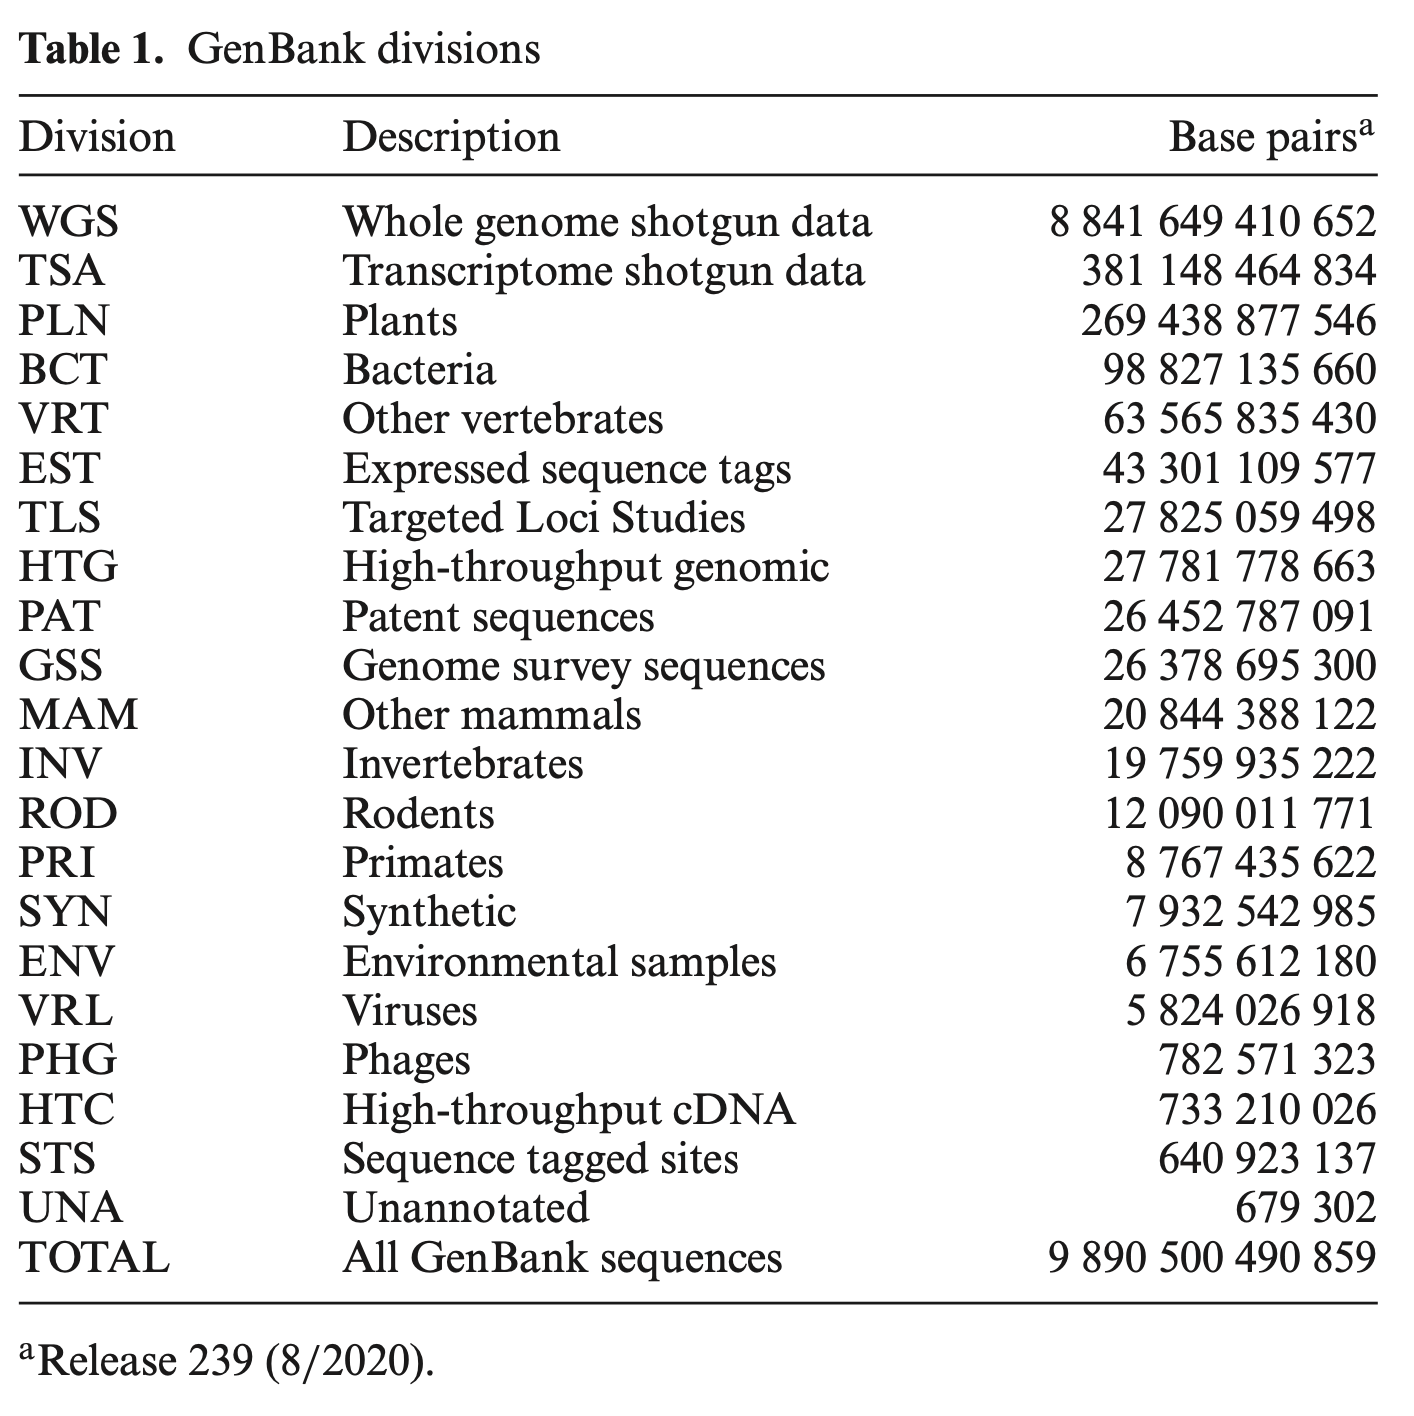
\includegraphics[width=5in]{figs/genbank-2020-table}

\end{center}

\vfill
\end{slide}
%%%%%%%%%%%%%%%%%%%%%%%%%%%%%%%%%%%%%%%%%%%%%%%%%%%%%%%%%%%%%%%%%%%%%%
\begin{slide}
\begin{center}
\textbf{Sequence submissions are handled by expert NCBI indexers}

\emph{but manual indexing does not scale}

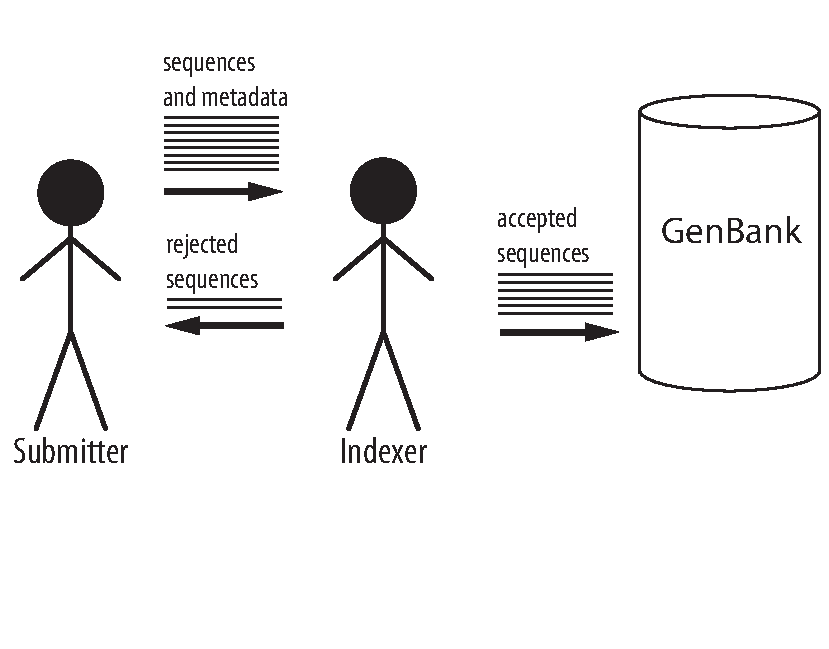
\includegraphics[width=7in]{figs/submission-schematic-1}

%\begin{itemize}
%\item Indexers check submissions for quality
%\end{itemize}

\vfill
\end{center}
\end{slide}
%%%%%%%%%%%%%%%%%%%%%%%%%%%%%%%%%%%%%%%%%%%%%%%%%%%%%%%%%%%%%%%%%%%%%%
\begin{slide}
\begin{center}
\large \textbf{Many submitted sequences are marker genes or viruses}
\end{center}
\medskip

\normalsize
\begin{center}
\begin{tabular}{lrr}
 marker gene/                    &  2021    & total \\
 virus                           &  \# seqs & \# seqs   \\ \hline
& & \\                    
SARS-CoV-2                     & 3,026,073 & 6,052,165 \\
& & \\
16S rRNA                        & 258,194 & 10,294,372 \\
& & \\                    
 23S rRNA                        & 59,191  & 1,236,112  \\
& & \\
 COX1                            & 86,248  & 541,630  \\
& & \\                    
 HIV-1                           & 44,359  & 1,035,342  \\
& & \\                    
 Influenza                       & 36,037  &   833,540  \\
& & \\                    
 ITS2                            & 26,630  &   260,245  \\
& & \\                    
 ITS1                            & 16,002  &   427,675  \\
& & \\                    
 ITS1+ITS2                       & 13,326  &   513,077  \\
\end{tabular}
\end{center}
\vfill
%\tiny \flushleft{$\dagger$ TLS: Targeted Locus Study, currently only 16S submissions with $>=$ 2500 seqs, handled by Anji Johnston}
%\tiny \flushleft{$\ddagger$ TLS submissions now processed with ribosensor}

% web entrez->nucleotide queries:
% 16S:
% all:  10,294,372 "(16S) NOT (LSU) NOT(18S) NOT (ITS1) NOT (ITS2) NOT (23S) NOT (28S)"
% 2021:    258,194 "(16S) NOT (LSU) NOT(18S) NOT (ITS1) NOT (ITS2) NOT (23S) NOT (28S) AND 2022/01/01:2022/12/31 [Publication Date]"
%
% SARS-CoV-2:
% all:   6,052,165 "txid694009[Organism:exp]"
% 2021:  3,026,073 "txid694009[Organism:exp] AND 2022/01/01:2022/12/31 [Publication Date] "
% 
% 23S:
% all:   1,236,112 "(23S) NOT (SSU) NOT(18S) NOT (ITS1) NOT (ITS2) NOT % (16S) NOT (28S)"
% 2021:     59,191 "(23S) NOT (SSU) NOT(18S) NOT (ITS1) NOT (ITS2) NOT % (16S) NOT (28S) AND 2022/01/01:2022/12/31 [Publication Date]""
%
% Cox1:
% all:     541,630 "cox1"
% 2021:     86,248 "cox1 AND 2022/01/01:2022/12/31 [Publication Date]"
%
% ITS1:
% all:     427,675 "(ITS1) NOT (LSU) NOT(18S) NOT (23S) NOT (ITS2) NOT (16S) NOT (28S) "
% 2021:     16,002 "(ITS1) NOT (LSU) NOT(18S) NOT (23S) NOT (ITS2) NOT (16S) NOT (28S) AND 2022/01/01:2022/12/31 [Publication Date]"
%
% ITS2:   
% all:     260,245 "(ITS2) NOT (LSU) NOT(18S) NOT (23S) NOT (ITS1) NOT (16S) NOT (28S)"
% 2021:     26,630 "(ITS2) NOT (LSU) NOT(18S) NOT (23S) NOT (ITS1) NOT (16S) NOT (28S) AND 2022/01/01:2022/12/31 [Publication Date]"
%
% ITS1+ITS2:
% all:     513,077 "(ITS1) AND (ITS2)"
% 2021:     13,236 "(ITS1) AND (ITS2) AND 2022/01/01:2022/12/31 [Publication Date]"
%
% Influenza:
% all:     833,540 "txid197911[Organism:exp]"
% 2021:     36,037 "txid197911[Organism:exp] AND 2022/01/01:2022/12/31 [Publication Date]
%
% HIV-1
% all:   1,035,342 "txid11676[Organism:exp]"
% 2021:     44,359 "txid11676[Organism:exp] AND 2022/01/01:2022/12/31 [Publication Date]




\end{slide}
%%%%%%%%%%%%%%%%%%%%%%%%%%%%%%%%%%%%%%%%%%%%%%%%%%%%%%%%%%%%%%%%%%%%%%
\begin{slide}
\begin{center}
\textbf{NCBI GenBank Indexers use BLAST}

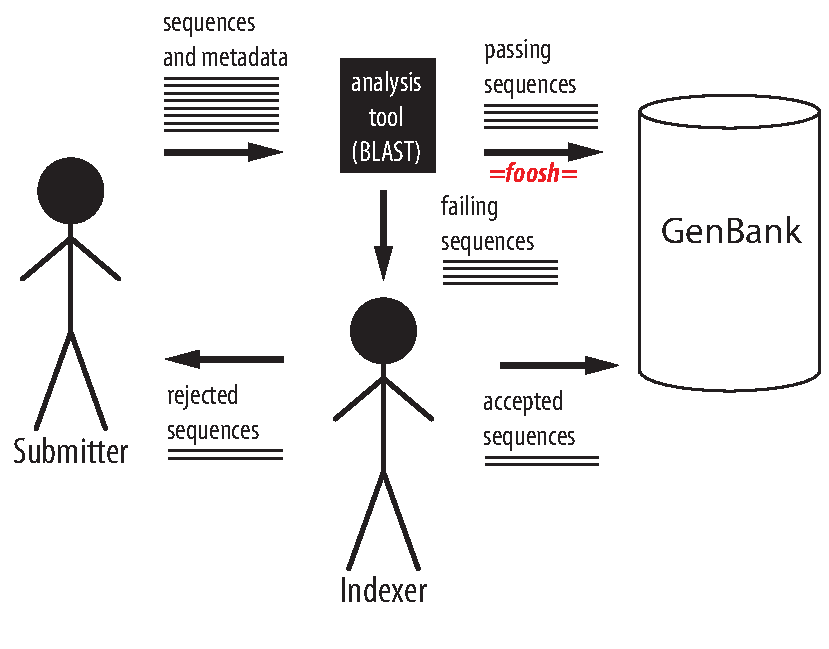
\includegraphics[width=7in]{figs/submission-schematic-2}

\small
\begin{itemize}
\item Foosh pipelines exist for 16S, 23S, ITS (BLAST-based) and
    Influenza (FLAN)
\end{itemize}

\vfill
\end{center}
\end{slide}
%%%%%%%%%%%%%%%%%%%%%%%%%%%%%%%%%%%%%%%%%%%%%%%%%%%%%%%%%%%%%%%%%%%%%%
%\begin{slide}
%\begin{center}
%\textbf{NCBI GenBank Indexers use BLAST}
%
%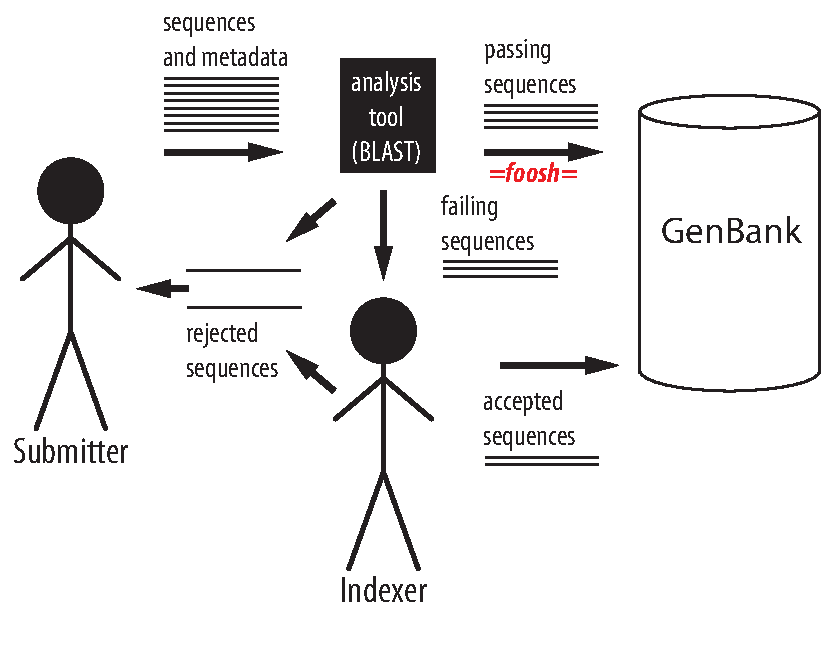
\includegraphics[width=7in]{figs/submission-schematic-3}
%
%\small
%\begin{itemize}
%\item Foosh pipelines exist for 16S, 23S, ITS (BLAST-based) and
%    Influenza (FLAN)
%\end{itemize}
%
%\vfill
%\end{center}
%\end{slide}
%%%%%%%%%%%%%%%%%%%%%%%%%%%%%%%%%%%%%%%%%%%%%%%%%%%%%%%%%%%%%%%%%%%%%%
\begin{slide}
\begin{center}

\textbf{Viruses with highest number of sequences in INSDC\footnote{as of August, 2022.}}

\tiny
\begin{tabular}{lrl}
species                   &       \#seqs & family           \\ \hline
%                                                              % taxids
& & \\
SARS-CoV-2                &     6,052,165& \emph{Coronaviridae}    \\ % 694009
& & \\
HIV-1                     &     1,035,342& \emph{Retroviridae}     \\ % 11676
& & \\
Influenza A virus         &      833,505 & \emph{Orthomyxoviridae} \\ % 11320
& & \\
Hepacivirus C             &      259,870 & \emph{Flaviviridae}     \\ % 11103
& & \\
Hepatitis B virus         &      124,490 & \emph{Hepadnaviridae}   \\ % 10407
& & \\
Influenza B virus         &      118,799 & \emph{Orthomyxoviridae} \\ % 11520
& & \\
Rotavirus A               &       96,690 & \emph{Reoviridae}       \\ % 28875
& & \\
Norovirus (Norwalk virus) &       51,748 & \emph{Caliciviridae}    \\ % 11983
& & \\
SIV                       &       50,454 & \emph{Retroviridae}     \\ % 11723
& & \\
West Nile virus           &       49,579 & \emph{Flaviviridae}     \\ % 11082
& & \\
Dengue virus              &       39,830 & \emph{Flaviviridae}     \\ % 12637
& & \\
Enterovirus A             &       39,527 & \emph{Picornaviridae}   \\ % 138948
& & \\
PRRSV                     &       38,538 & \emph{Arteriviridae}    \\ % 28344
& & \\
Human orthopneumovirus    &       32,835 & \emph{Pneumoviridae}    \\ % 11250 (RSV) 
& & \\
Enterovirus B             &       28,494 & \emph{Picornaviridae}   \\ % 138949
& & \\
Lyssavirus rabies         &       26,798 & \emph{Rhabdoviridae}    \\ % 11292
\end{tabular}

\vfill

\end{center}
\end{slide}

%%%%%%%%%%%%%%%%%%%%%%%%%%%%%%%%%%%%%%%%%%%%%%%%%%%%%%%%%%%%%%%%%%%%%%
\begin{slide}
\begin{center}
\textbf{Viral sequences are not systematically or thoroughly annotated}
\end{center}
\medskip

\small
\begin{itemize}
\item Genome annotation of the Zika virus:
\end{itemize}  

\center{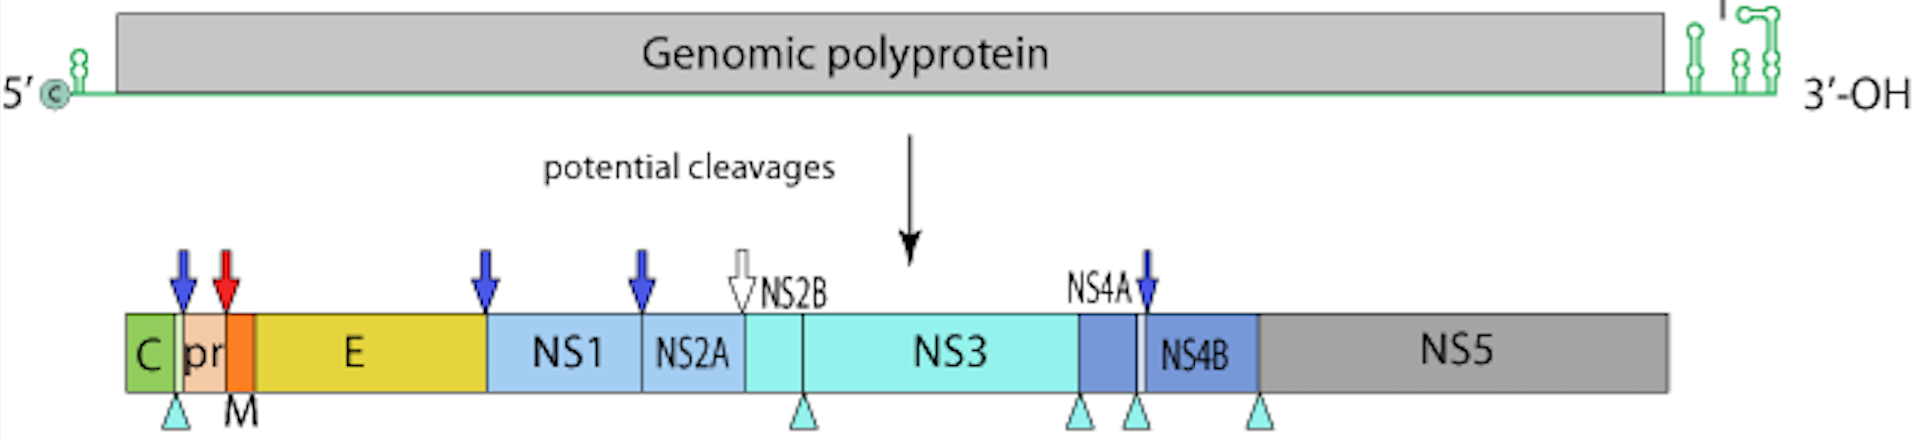
\includegraphics[width=8in]{figs/zika-genome-norna}}

\begin{itemize}
\item Zika's genome encodes a single polyprotein that is cleaved into 14 mature peptides.
\item Zika RefSeq annotation (NC\_012532) includes CDS and mature peptide annotation.
\end{itemize}

\vfill
\tiny \flushleft{figure from ViralZone, Hulo et al. NAR. 2011 Jan;39:D576-82}
\end{slide}
%%%%%%%%%%%%%%%%%%%%%%%%%%%%%%%%%%%%%%%%%%%%%%%%%%%%%%%%%%%%%%%%%%%%%%
\begin{slide}
\begin{center}
\textbf{Viral sequences are not systematically or thoroughly annotated}
\end{center}
\medskip

\small
\begin{itemize}
\item Genome annotation of the Zika virus:
\end{itemize}  

\center{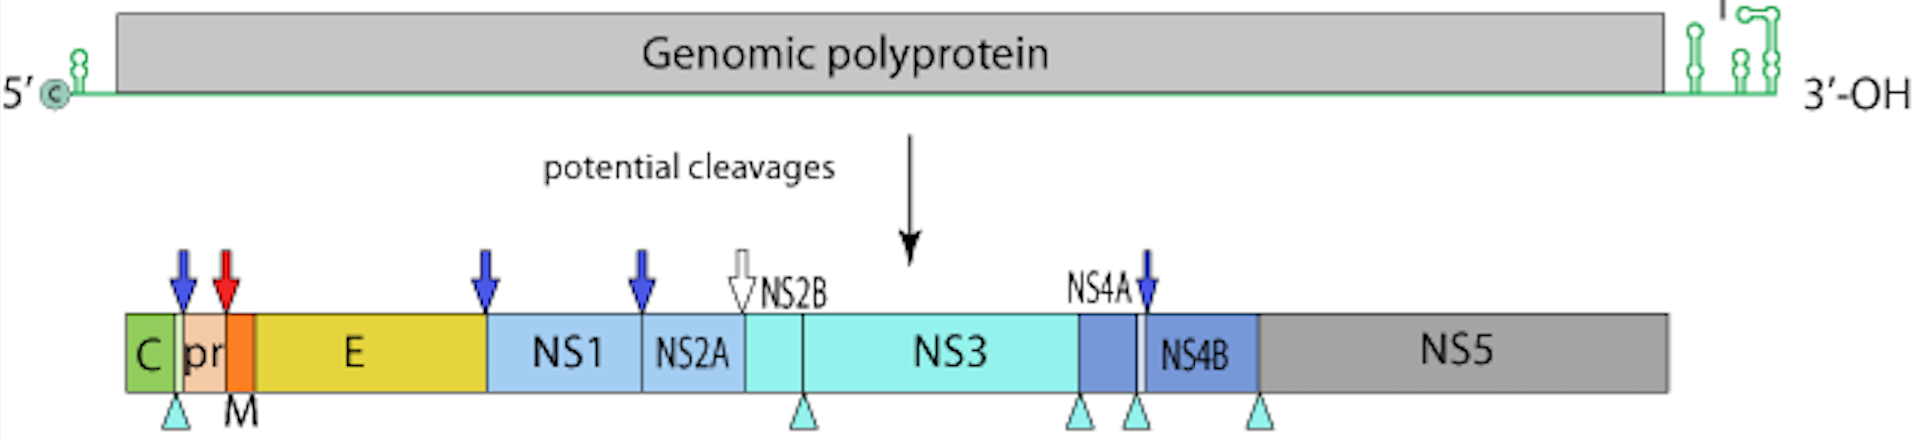
\includegraphics[width=8in]{figs/zika-genome-norna}}

\begin{itemize}
\item Zika's genome encodes a single polyprotein that is cleaved into 14 mature peptides.
\item Zika RefSeq annotation (NC\_012532) includes CDS and mature peptide annotation.
\item About 84\% of Zika virus sequences have CDS annotation.
\item Less than 25\% of Zika virus sequences have mature peptide annotation.
\item Less than 7\% of Dengue virus sequences have mature peptide annotation.
\item Less than 2\% of Norovirus sequences have mature peptide annotation.
\end{itemize}

\vfill
\tiny \flushleft{figure from ViralZone, Hulo et al. NAR. 2011 Jan;39:D576-82}
\end{slide}
%%%%%%%%%%%%%%%%%%%%%%%%%%%%%%%%%%%%%%%%%%%%%%%%%%%%%%%%%%%%%%%%%%%%
\begin{slide}
\begin{center}
\textbf{Viral sequences are not systematically or thoroughly annotated}
\end{center}
\medskip

\small
\begin{itemize}
\item Genome annotation of the Zika virus:
\end{itemize}  

\center{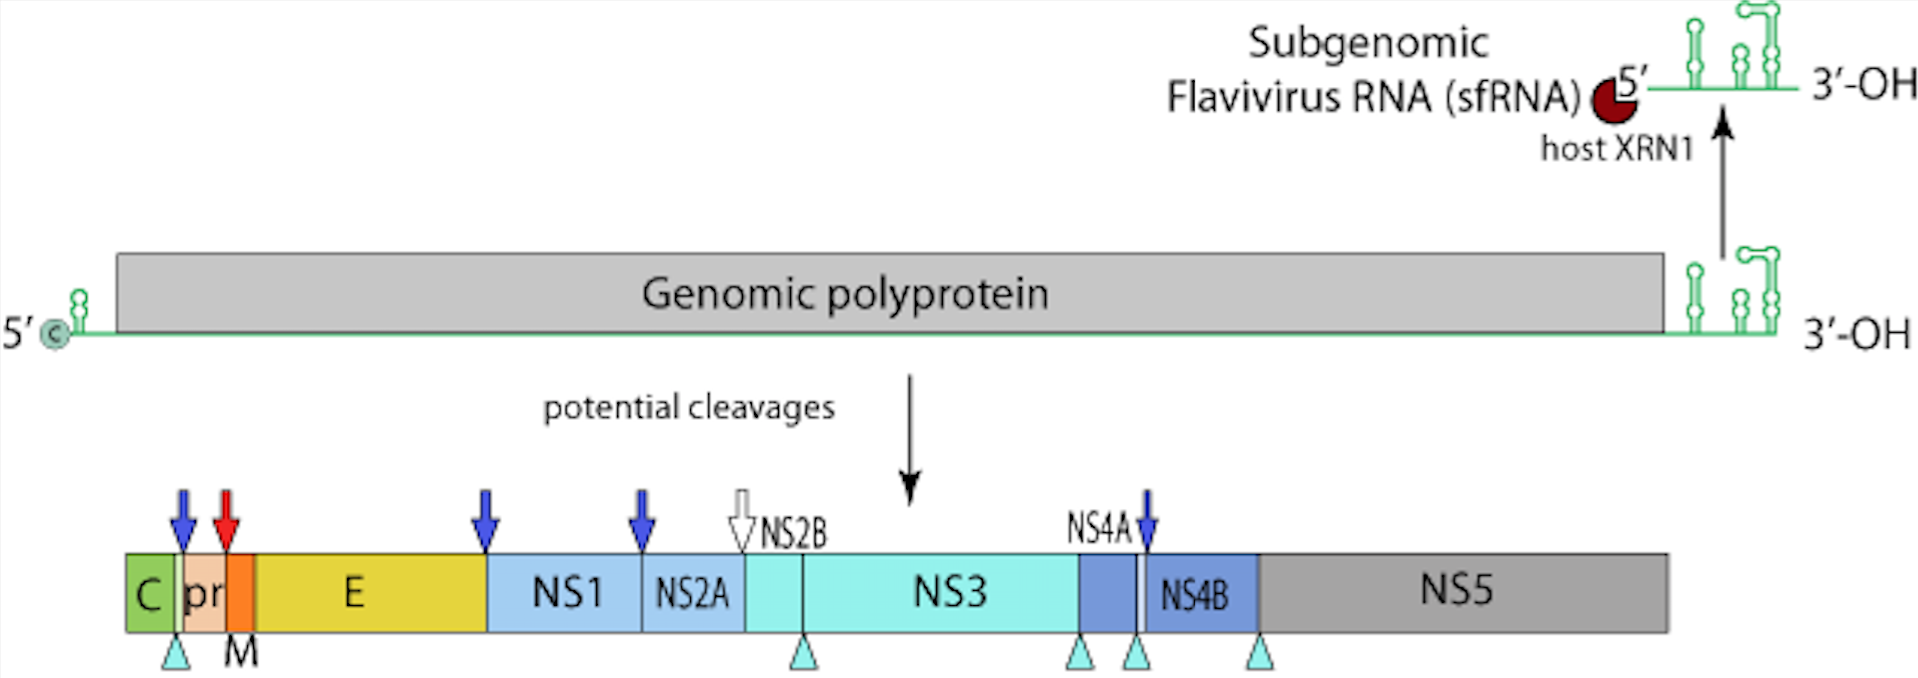
\includegraphics[width=8in]{figs/zika-genome-yesrna}}

\begin{itemize}
\item RNA structures in the 3' UTR halt host exonuclease leading to an
  accumulation of 300-500nt subgenomic flavivirus RNAs (sfRNAs) are
  related to pathogenicity.
\end{itemize}

\normalsize
\center{\textbf{\emph{These RNA structures are not annotated in the
      \\ Zika genome RefSeq (NC\_012532)}}}

\vfill
\tiny \flushleft{figure from ViralZone, Hulo et al. NAR. 2011 Jan;39:D576-82}
\end{slide}
%%%%%%%%%%%%%%%%%%%%%%%%%%%%%%%%%%%%%%%%%%%%%%%%%%%%%%%%%%%%%%%%%%%%%%
\begin{slide}
\begin{center}
\textbf{Viral sequences are not systematically or thoroughly annotated}
\end{center}

\small
\begin{itemize}
\item CDS are not always annotated
\item Mature peptides are rarely annotated
\item Rfam families are rarely to never annotated in viral genomes
  (more than 200 families)
\end{itemize}

\normalsize
\center{\textbf{\emph{Systematic and complete annotation would \\ benefit viral
  researchers (facilitate comparative analyses)}}}

\vfill
\end{slide}
%%%%%%%%%%%%%%%%%%%%%%%%%%%%%%%%%%%%%%%%%%%%%%%%%%%%%%%%%%%%%%%%%%%%%%
\begin{slide}
\begin{center}
\textbf{Annotation and validation should be coupled}
\end{center}

\begin{center}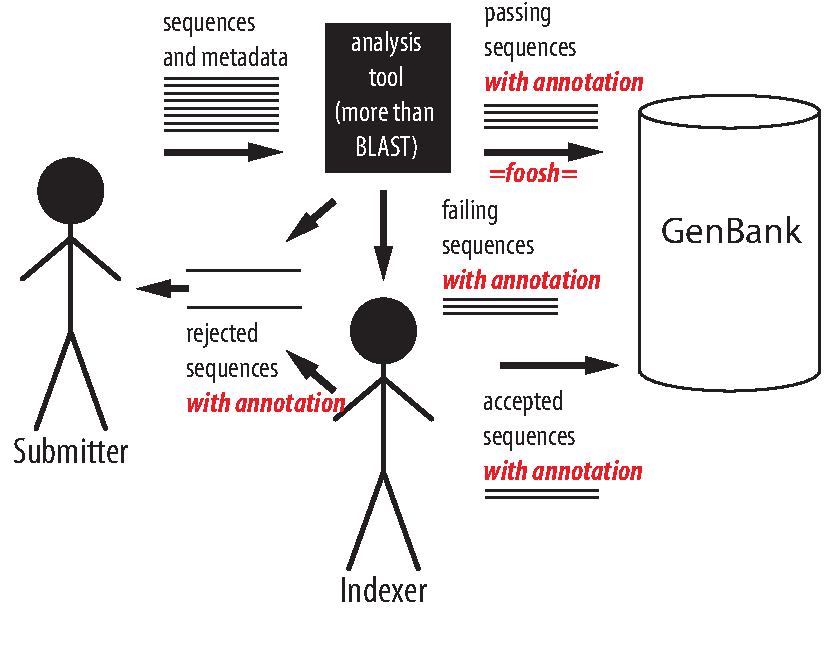
\includegraphics[width=7in]{figs/submission-schematic-4}\end{center}

\vfill
\end{slide}
%%%%%%%%%%%%%%%%%%%%%%%%%%%%%%%%%%%%%%%%%%%%%%%%%%%%%%%%%%%%%%%%%%%%%%
\begin{slide}
\begin{center}

\includegraphics[width=6in]{figs/vadr-title-paper}
%\textbf{VADR (Viral Annotation DefineR) \\ uses RefSeqs to validate and
%annotate viral sequences}

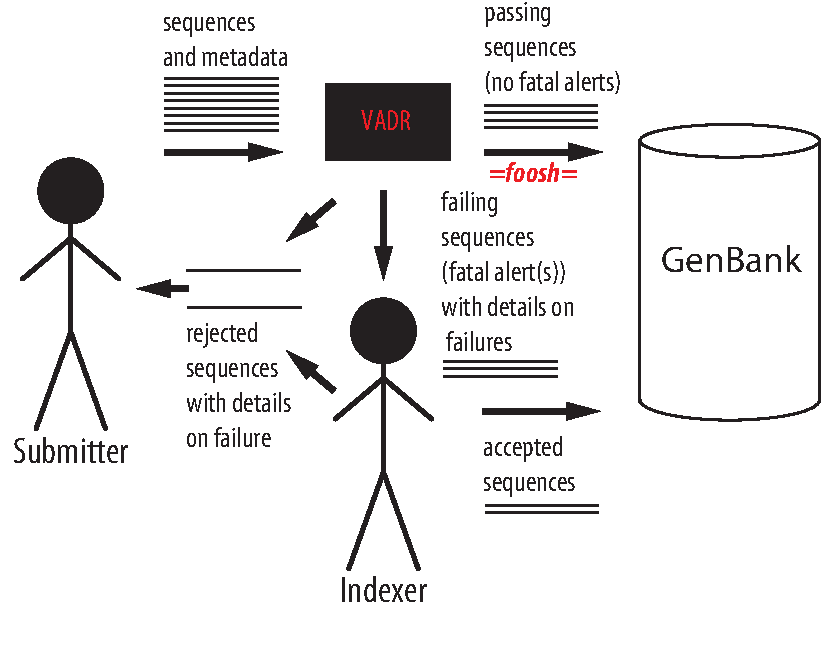
\includegraphics[width=6in]{figs/submission-schematic-5}
\end{center}

\small
\begin{itemize}
  \item Unexpected characteristics are reported as \emph{alerts}
    (e.g. early stop codon), some of which are \emph{fatal} and cause
    sequences to \emph{fail}
   %\item Some alerts are \emph{fatal} and cause sequences to \emph{fail}
\end{itemize}

%\small
%\begin{itemize}
%\item Build a model (covariance model) from a RefSeq (or alignment) using \texttt{v-build.pl}
%\begin{itemize}
%  \item includes boundaries of CDS, mat\_peptide, ncRNA and other features
%\end{itemize}

%\item Incoming sequences are compared against a library of models to find
%  the best-matching model which is used to annotate the sequence using
%  \texttt{v-annotate.pl}.

\vfill
\end{slide}
%%%%%%%%%%%%%%%%%%%%%%%%%%%%%%%%%%%%%%%%%%%%%%%%%%%%%%%%%%%%%%%%%%%%%%
\begin{slide}
\begin{center}

\textbf{Norovirus and Dengue virus chosen as first viruses for VADR testing}

\tiny
\begin{tabular}{lrl}
species                   &       \#seqs & family           \\ \hline
%                                                              % taxids
& & \\
SARS-CoV-2                &     6,045,832& \emph{Coronaviridae}    \\ % 694009
& & \\
HIV-1                     &     1,033,995& \emph{Retroviridae}     \\ % 11676
& & \\
Influenza A virus         &      833,505 & \emph{Orthomyxoviridae} \\ % 11320
& & \\
Hepacivirus C             &      259,870 & \emph{Flaviviridae}     \\ % 11103
& & \\
Hepatitis B virus         &      124,490 & \emph{Hepadnaviridae}   \\ % 10407
& & \\
Influenza B virus         &      118,799 & \emph{Orthomyxoviridae} \\ % 11520
& & \\
Rotavirus A               &       96,690 & \emph{Reoviridae}       \\ % 28875
& & \\
\textcolor{red}{Norovirus (Norwalk virus)} &       \textcolor{red}{51,748} & \textcolor{red}{\emph{Caliciviridae}}    \\ % 11983
& & \\
SIV                       &       50,454 & \emph{Retroviridae}     \\ % 11723
& & \\
West Nile virus           &       49,579 & \emph{Flaviviridae}     \\ % 11082
& & \\
\textcolor{red}{Dengue virus}              &       \textcolor{red}{39,830} & \textcolor{red}{\emph{Flaviviridae}}     \\ % 12637
& & \\
Enterovirus A             &       39,527 & \emph{Picornaviridae}   \\ % 138948
& & \\
PRRSV                     &       38,538 & \emph{Arteriviridae}    \\ % 28344
& & \\
Human orthopneumovirus    &       32,835 & \emph{Pneumoviridae}    \\ % 11250 (RSV) 
& & \\
Enterovirus B             &       28,494 & \emph{Picornaviridae}   \\ % 138949
& & \\
Lyssavirus rabies         &       26,798 & \emph{Rhabdoviridae}    \\ % 11292
\end{tabular}

\vfill

\end{center}
\end{slide}

%%%%%%%%%%%%%%%%%%%%%%%%%%%%%%%%%%%%%%%%%%%%%%%%%%%%%%%%%%%%%%%%%%%%%%
\begin{slide}
\begin{center}
\large{\textbf{VADR builds a reference model of a \\ RefSeq and its features}}
\end{center}

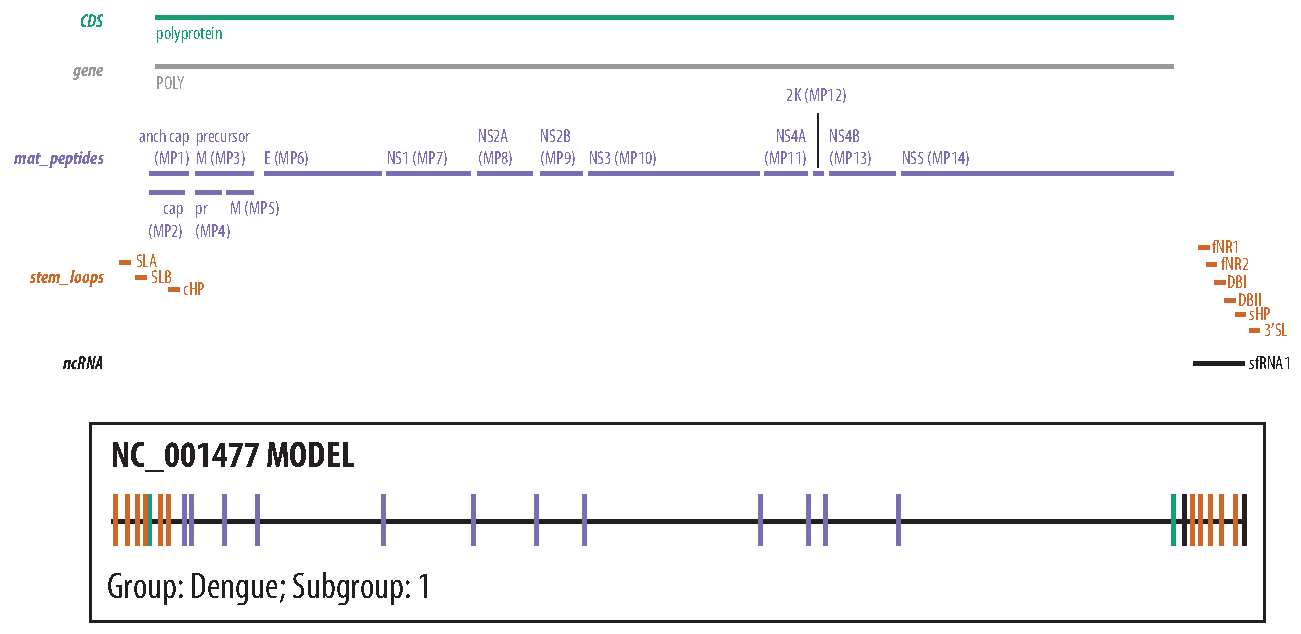
\includegraphics[width=10.5in]{figs/dengue-features}

\vfill
\end{slide}
%%%%%%%%%%%%%%%%%%%%%%%%%%%%%%%%%%%%%%%%%%%%%%%%%%%%%%%%%%%%%%%%%%%%%%
\begin{slide}
\begin{center}
%\textbf{\texttt{v-annotate.pl} annotates each sequence using its
\large{\textbf{VADR validates and annotates each input sequence \\ using its 
  best-matching model}}

\begin{itemize}
\item Each sequence $S$ proceeds through 4 stages:
%\item For each sequence $S$:
\small
\begin{enumerate}
%\item \textbf{Classification}: compare $S$ to all models to find best matching model $M$
\item \textbf{Classification}
%\item \textbf{Coverage determination}: search $M$ against $S$ to find 'hits'
\item \textbf{Coverage determination}
%\item \textbf{Alignment}: align $S$ to $M$ and map features from $M$ to $S$
\item \textbf{Alignment}
%\item \textbf{Protein validation}: compare predicted CDS in $S$ to proteins
\item \textbf{Protein validation}
\end{enumerate}
\end{itemize}

\normalsize
\emph{Different types of alerts are identified and reported at each stage}

\end{center}

\vfill
\end{slide}
%%%%%%%%%%%%%%%%%%%%%%%%%%%%%%%%%%%%%%%%%%%%%%%%%%%%%%%%%%%%%%%%%%%%%%
\begin{slide}
\begin{center}

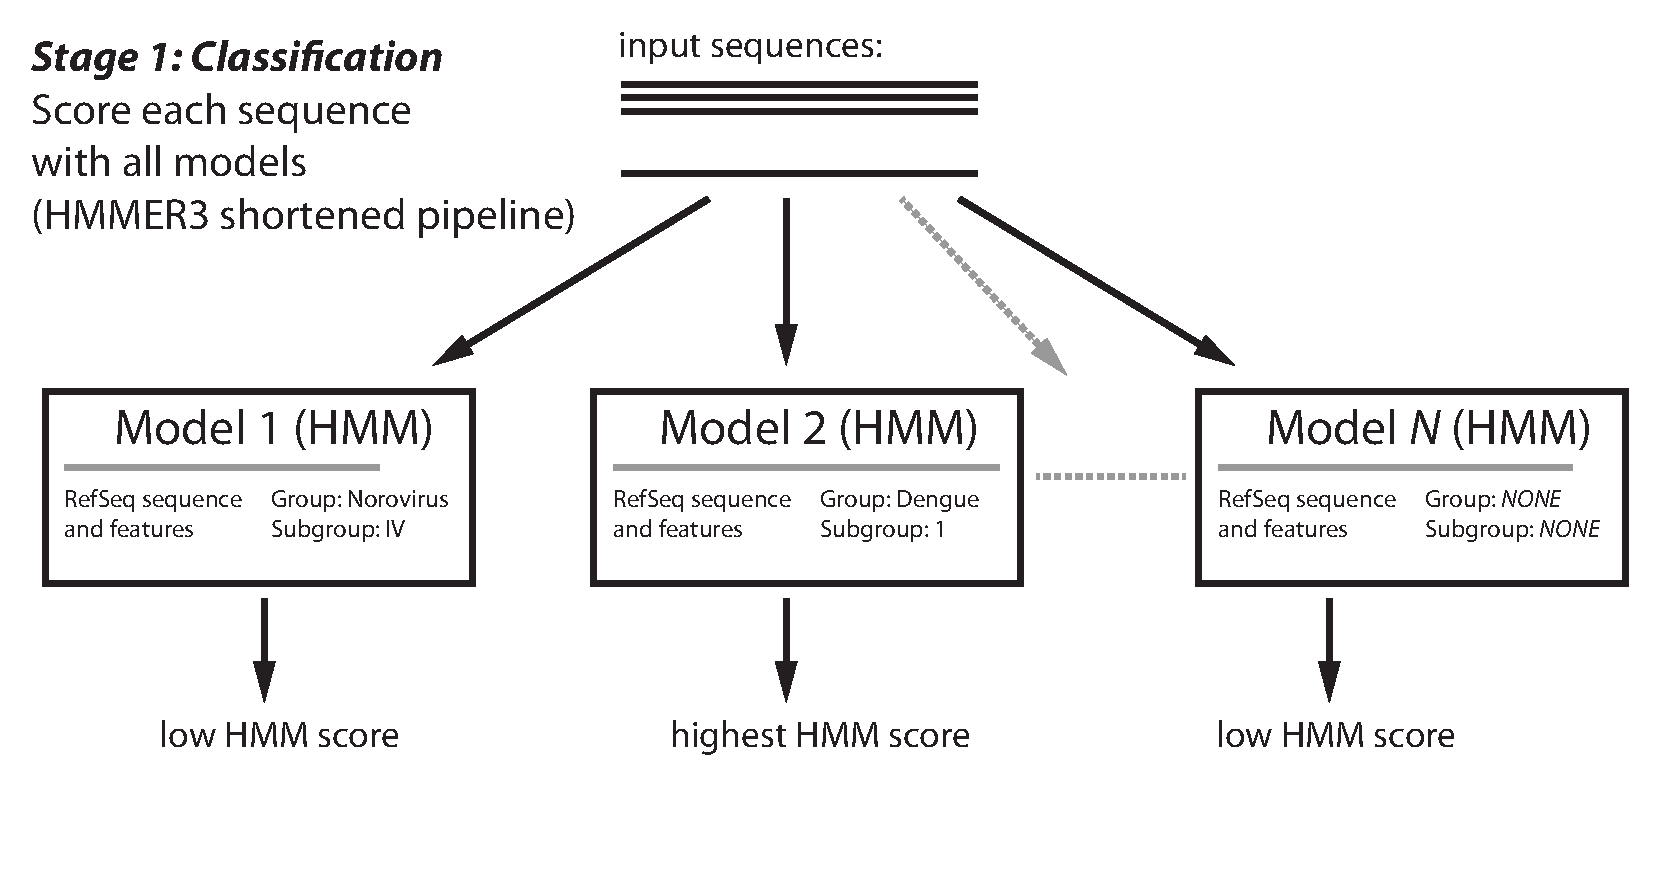
\includegraphics[width=9.5in]{figs/v-annotate-stage1-1}

\end{center}
\vfill
\end{slide}
%%%%%%%%%%%%%%%%%%%%%%%%%%%%%%%%%%%%%%%%%%%%%%%%%%%%%%%%%%%%%%%%%%%%%%
\begin{slide}
\begin{center}

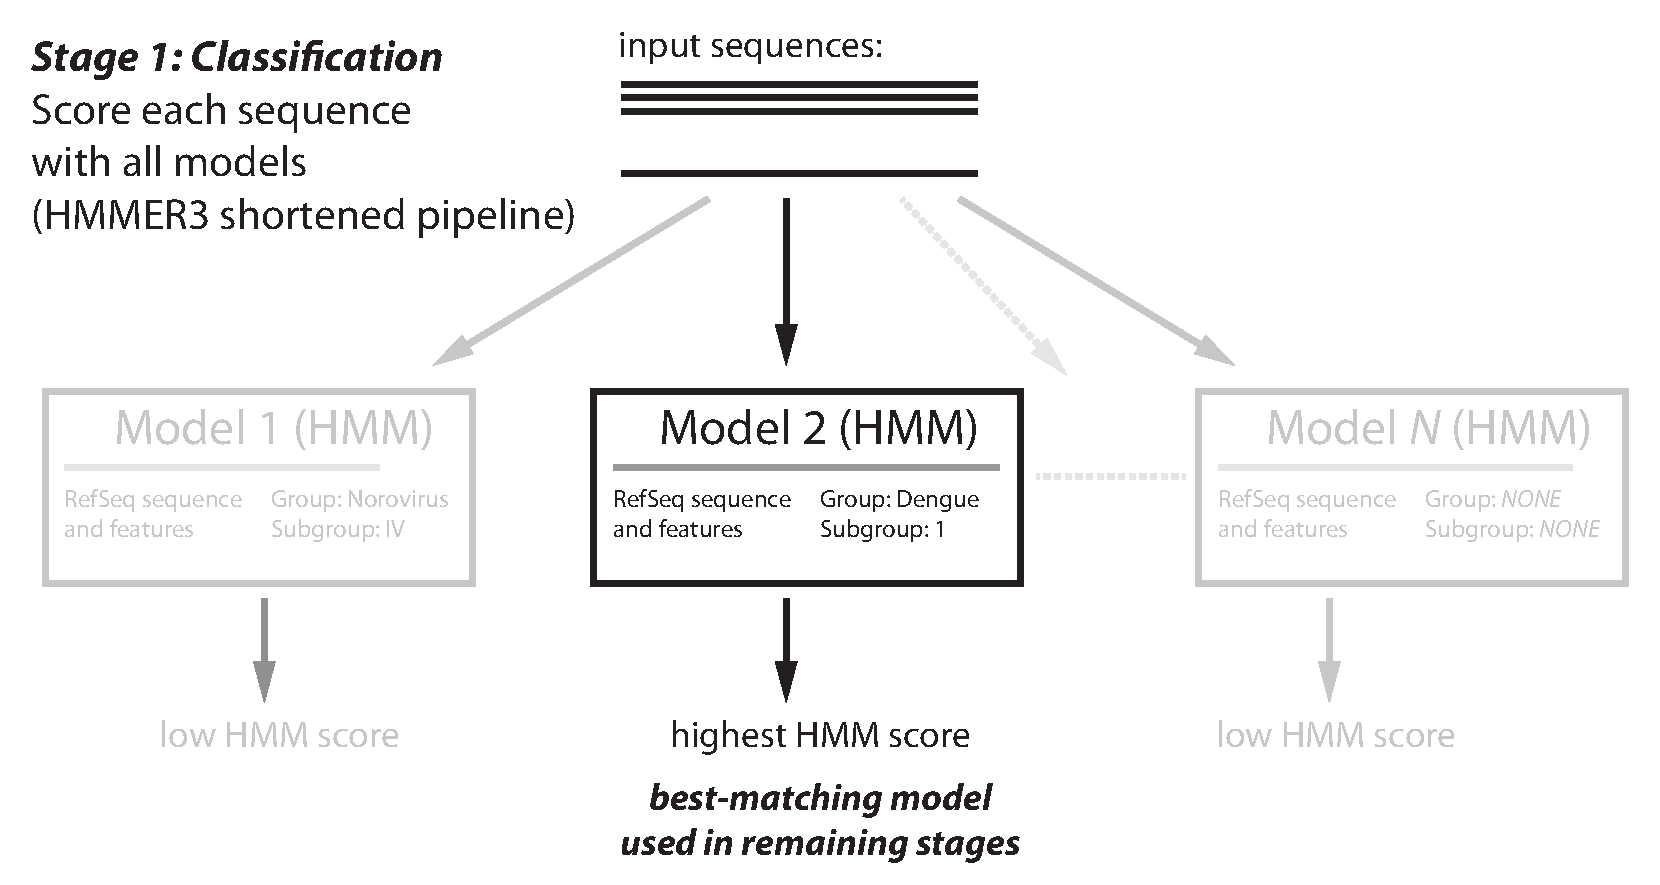
\includegraphics[width=9.5in]{figs/v-annotate-stage1-2}

\end{center}
\vfill
\end{slide}
%%%%%%%%%%%%%%%%%%%%%%%%%%%%%%%%%%%%%%%%%%%%%%%%%%%%%%%%%%%%%%%%%%%%%%
\begin{slide}
\begin{center}

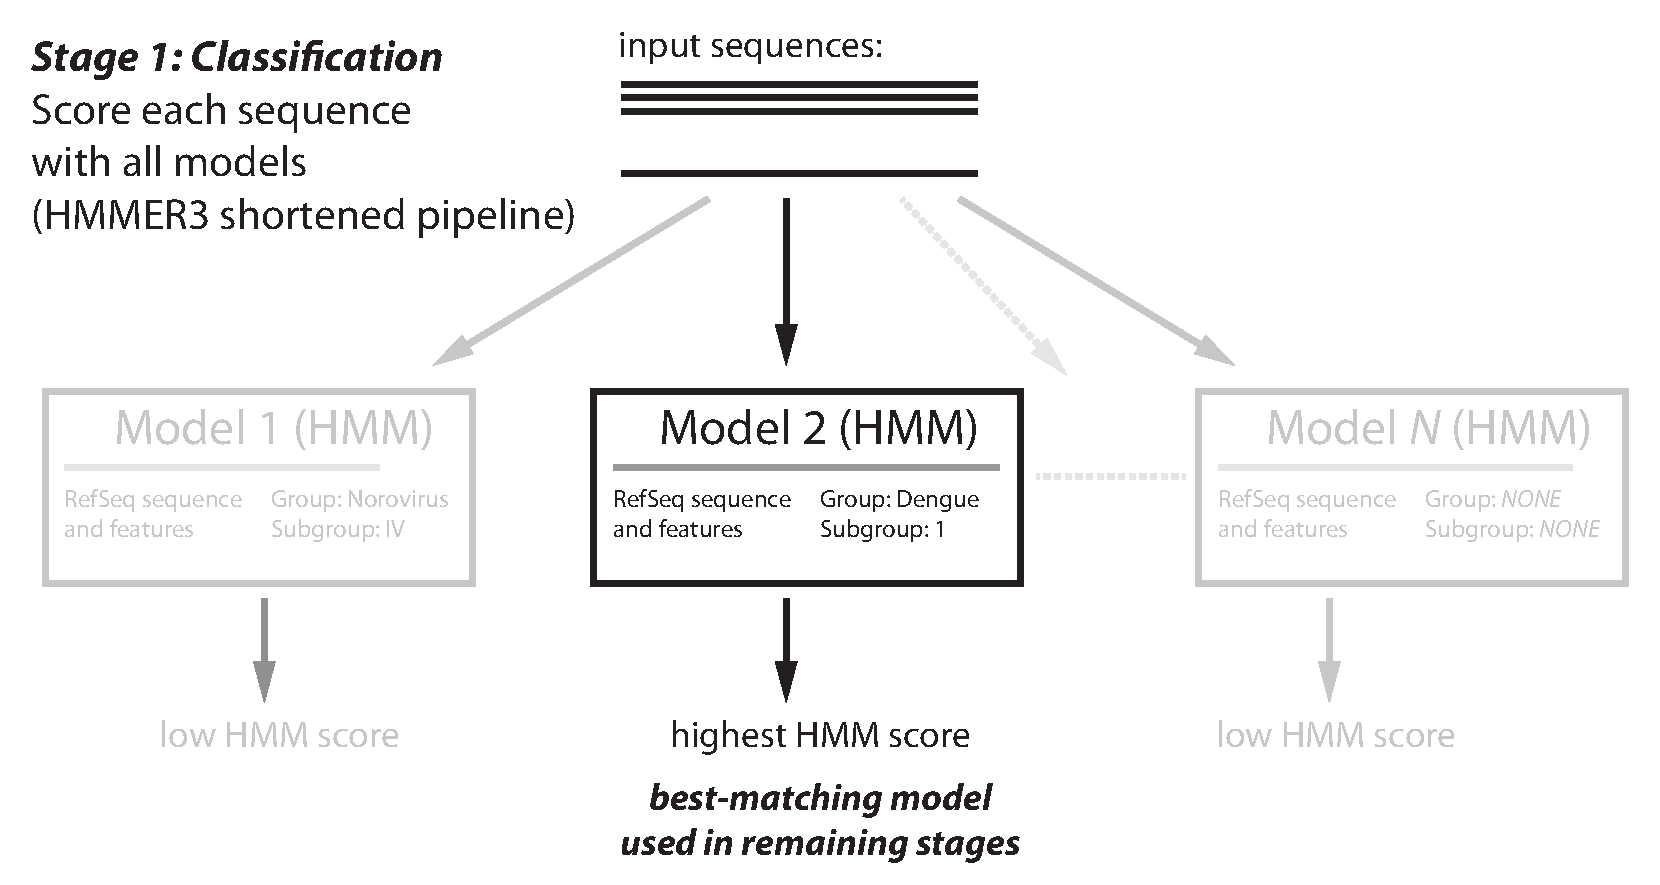
\includegraphics[width=9.5in]{figs/v-annotate-stage1-2}

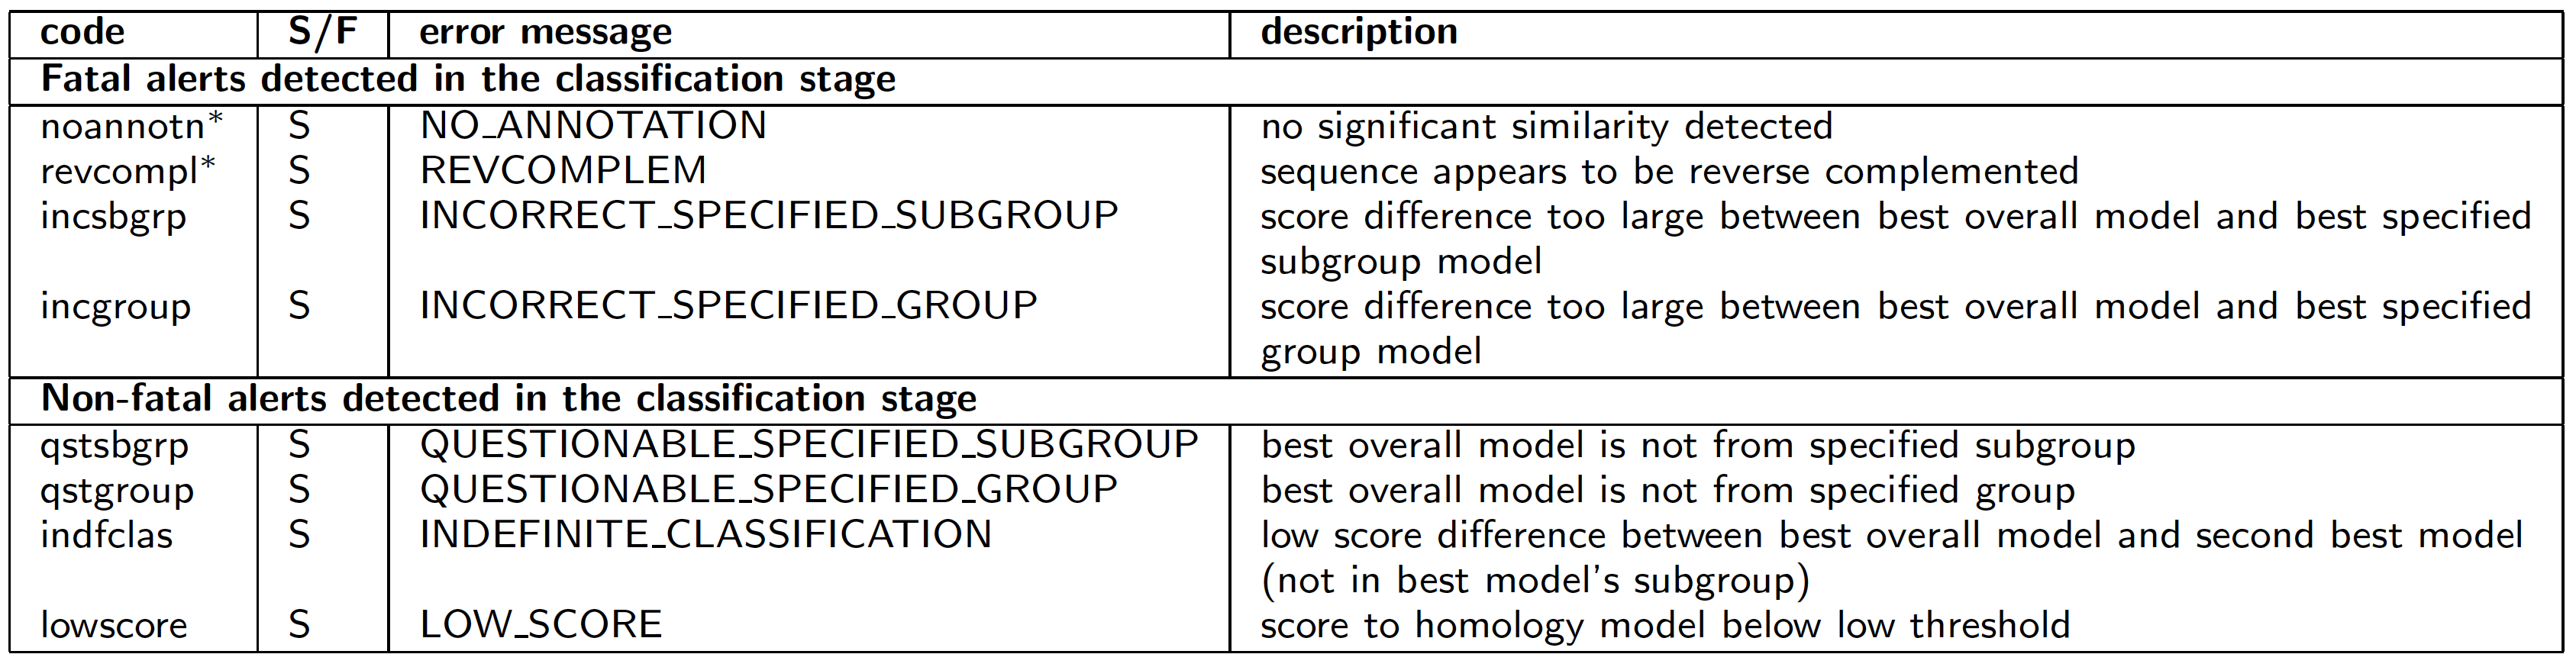
\includegraphics[width=10.5in]{figs/ss-class-alert-list}

\end{center}
\vfill
\end{slide}
%%%%%%%%%%%%%%%%%%%%%%%%%%%%%%%%%%%%%%%%%%%%%%%%%%%%%%%%%%%%%%%%%%%%%%
\begin{slide}
\begin{center}

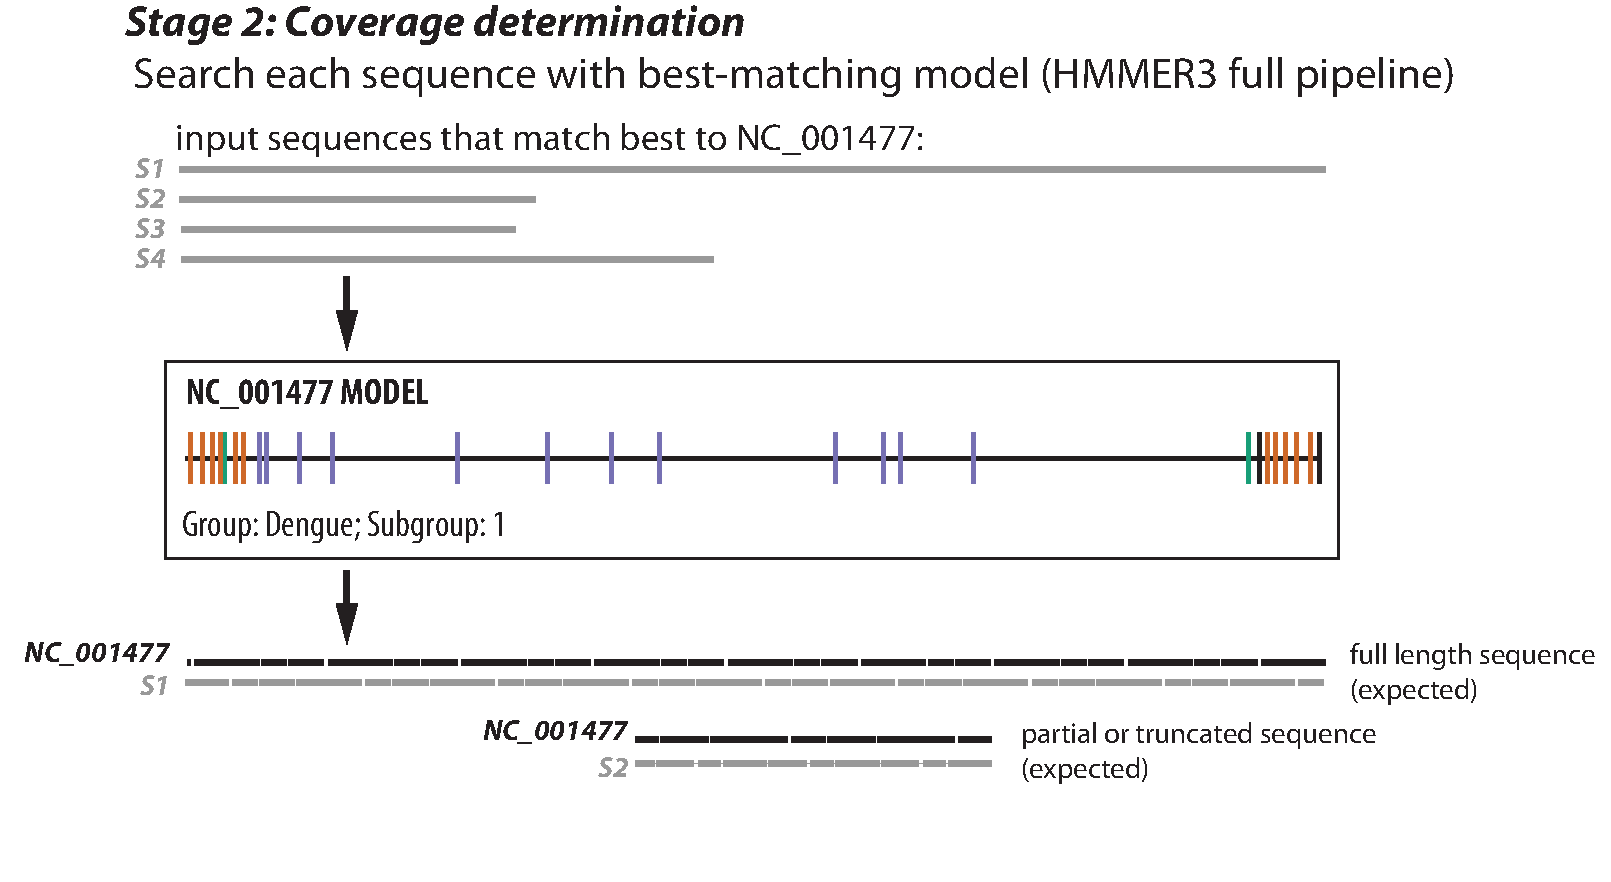
\includegraphics[width=10.5in]{figs/v-annotate-stage2-1}

\end{center}
\vfill
\end{slide}
%%%%%%%%%%%%%%%%%%%%%%%%%%%%%%%%%%%%%%%%%%%%%%%%%%%%%%%%%%%%%%%%%%%%%%
\begin{slide}
\begin{center}

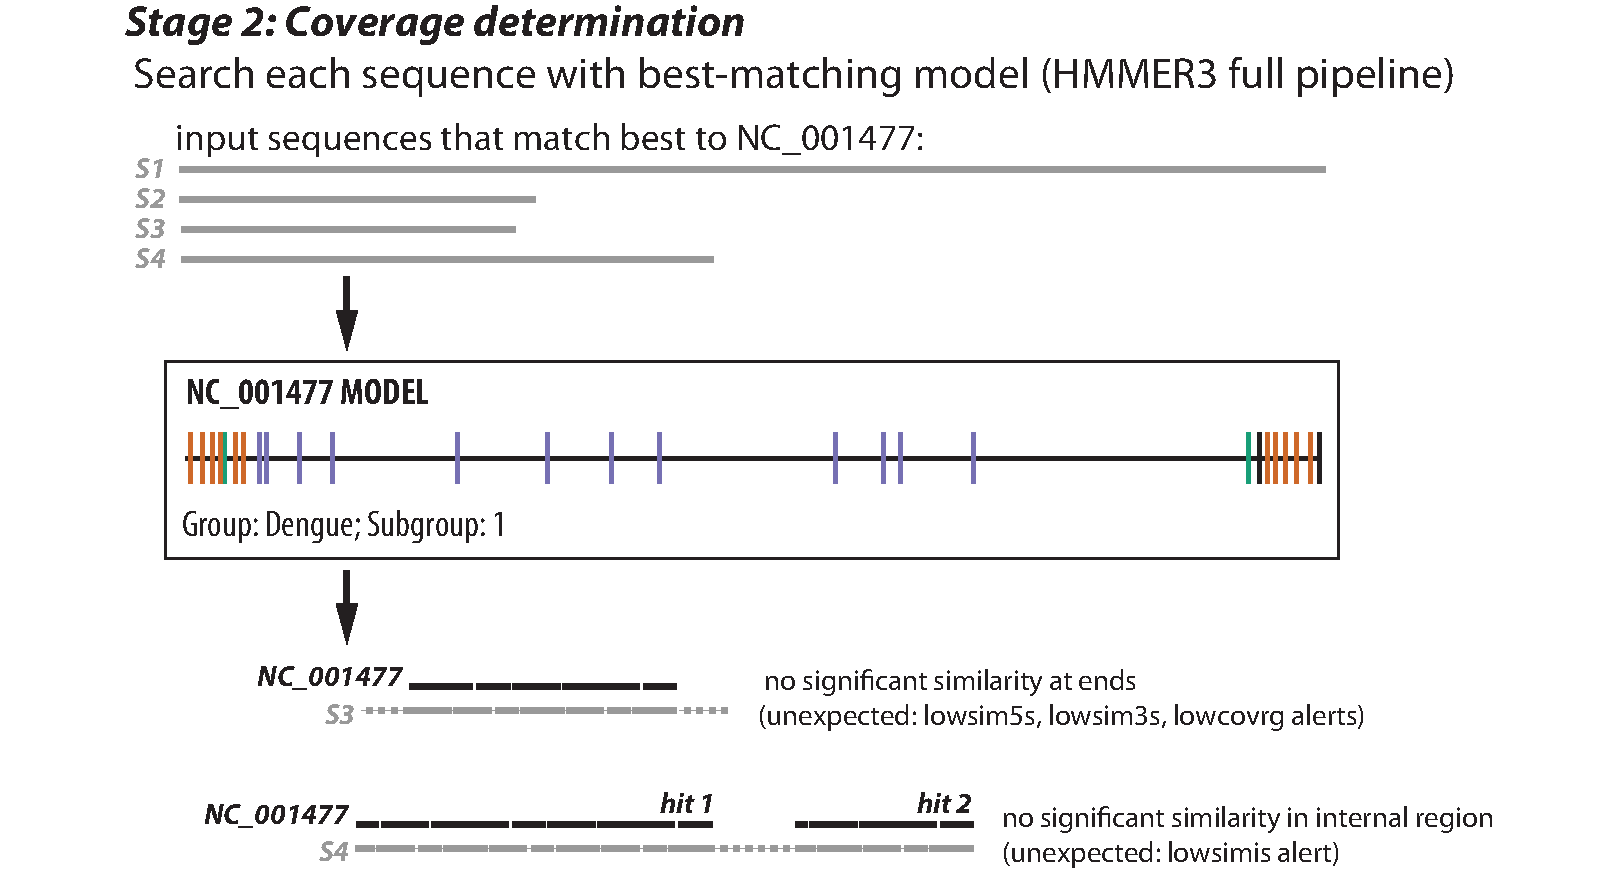
\includegraphics[width=10.5in]{figs/v-annotate-stage2-2}
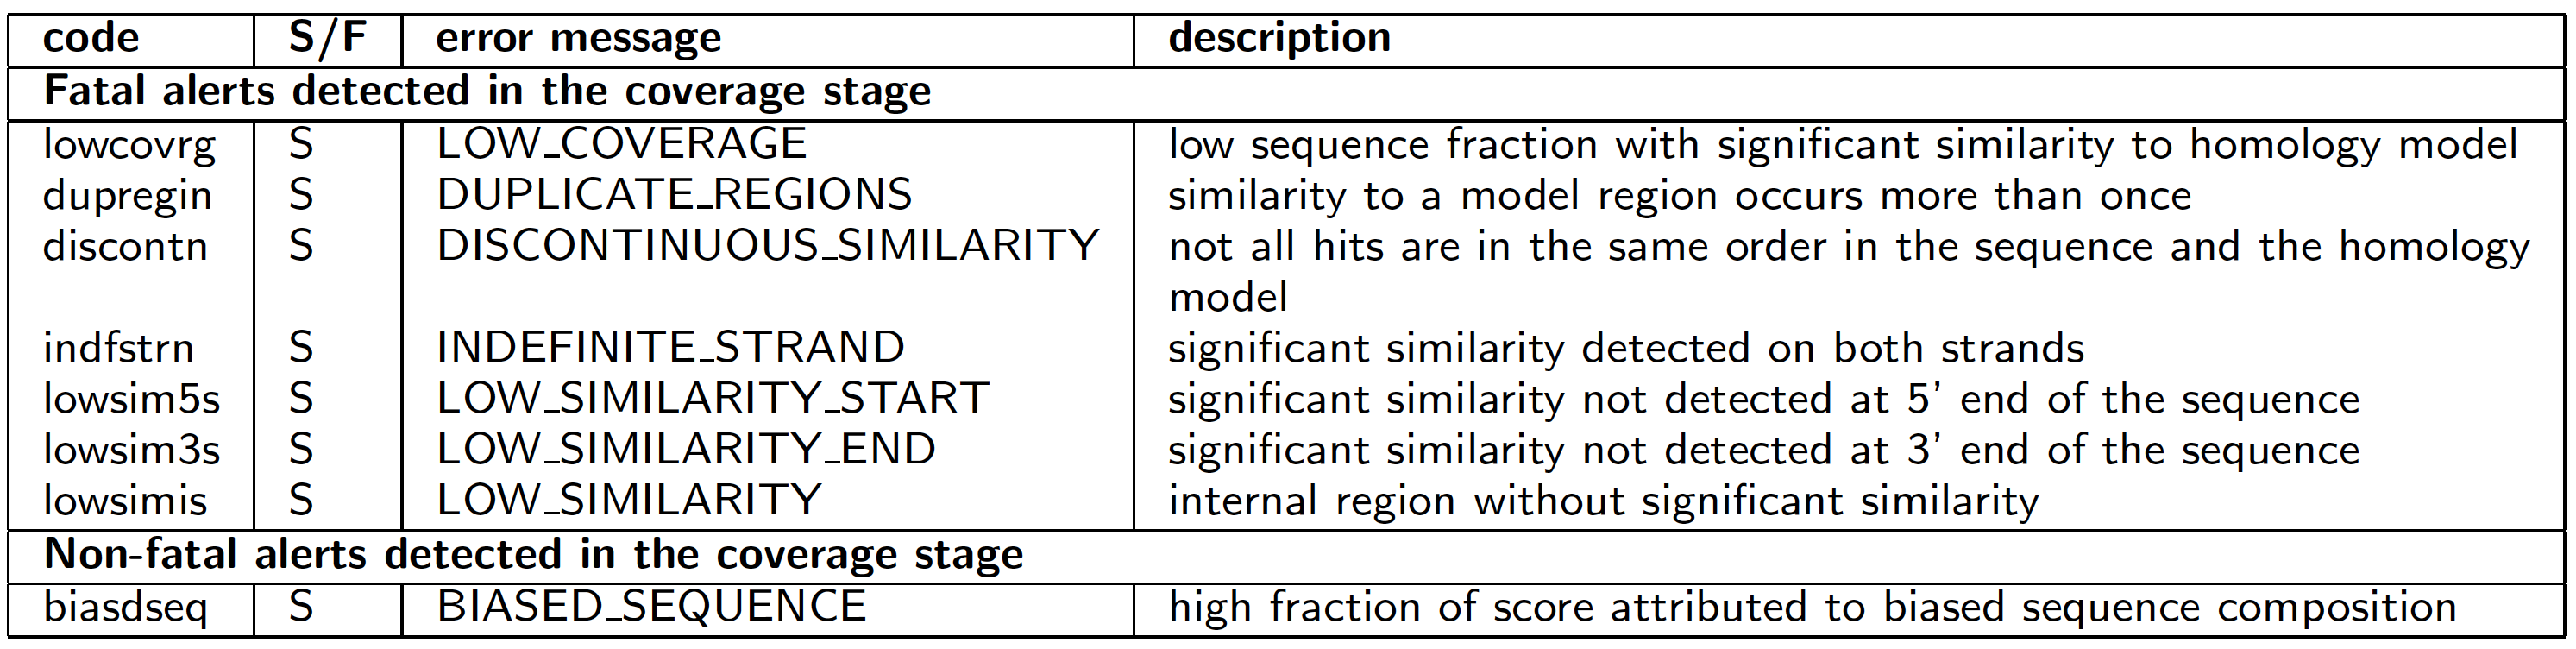
\includegraphics[width=10in]{figs/ss-coverage-alert-list}
\end{center}

\vfill
\end{slide}
%%%%%%%%%%%%%%%%%%%%%%%%%%%%%%%%%%%%%%%%%%%%%%%%%%%%%%%%%%%%%%%%%%%%%%
\begin{slide}
\begin{center}

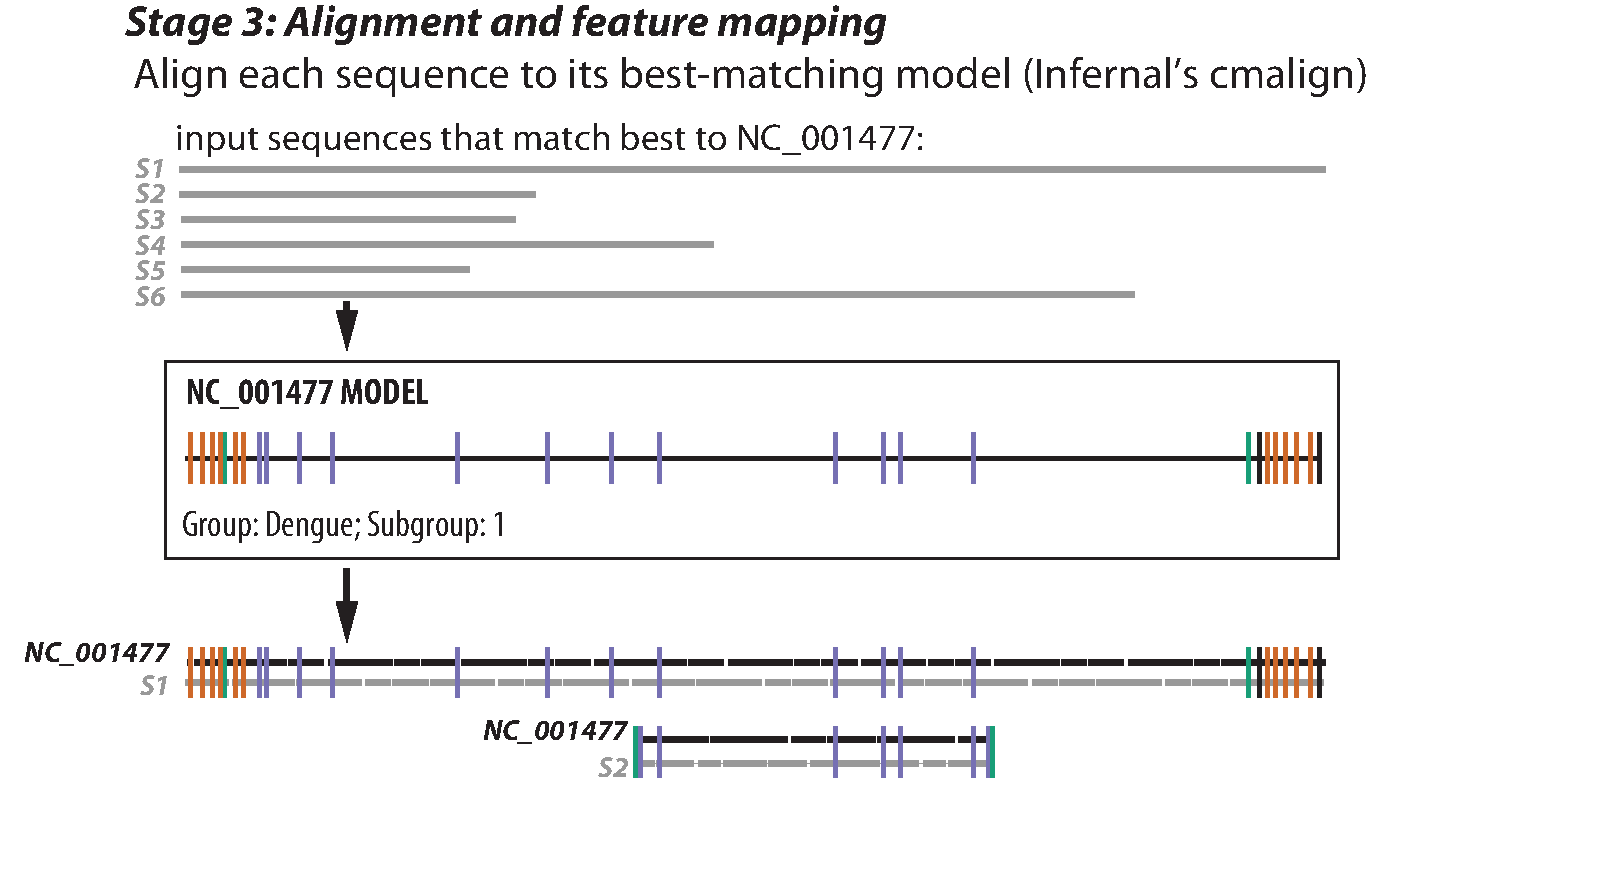
\includegraphics[width=10.5in]{figs/v-annotate-stage3-1}
\end{center}

\vfill
\end{slide}
%%%%%%%%%%%%%%%%%%%%%%%%%%%%%%%%%%%%%%%%%%%%%%%%%%%%%%%%%%%%%%%%%%%%%%
%\begin{slide}
%\begin{center}
%
%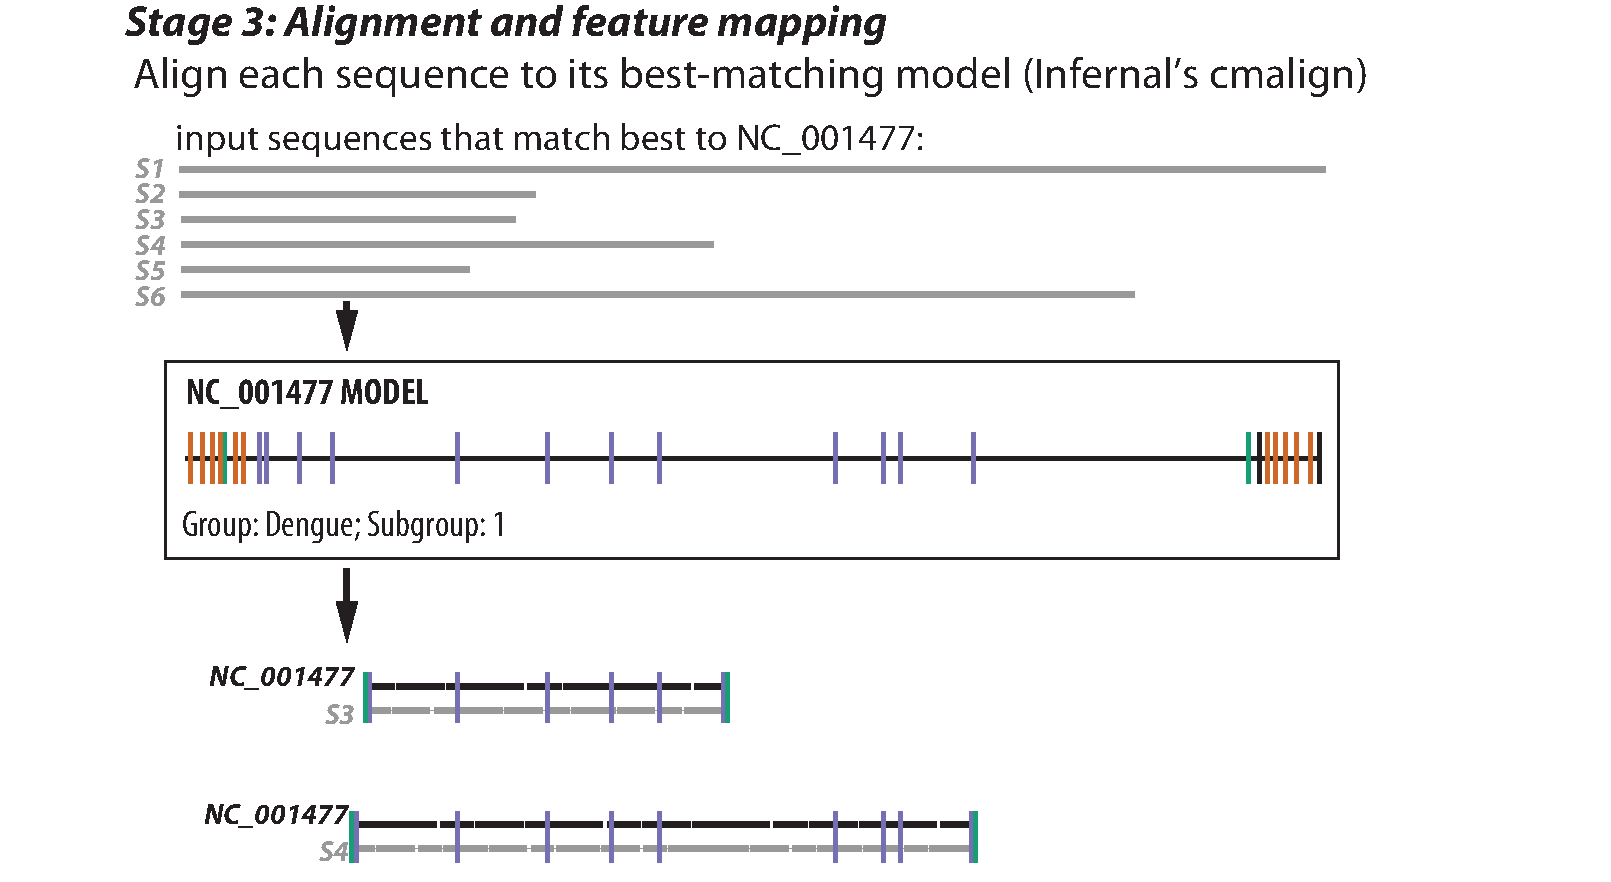
\includegraphics[width=10.5in]{figs/v-annotate-stage3-2}
%\end{center}
%
%\vfill
%\end{slide}
%%%%%%%%%%%%%%%%%%%%%%%%%%%%%%%%%%%%%%%%%%%%%%%%%%%%%%%%%%%%%%%%%%%%%%
%\begin{slide}
%\begin{center}
%
%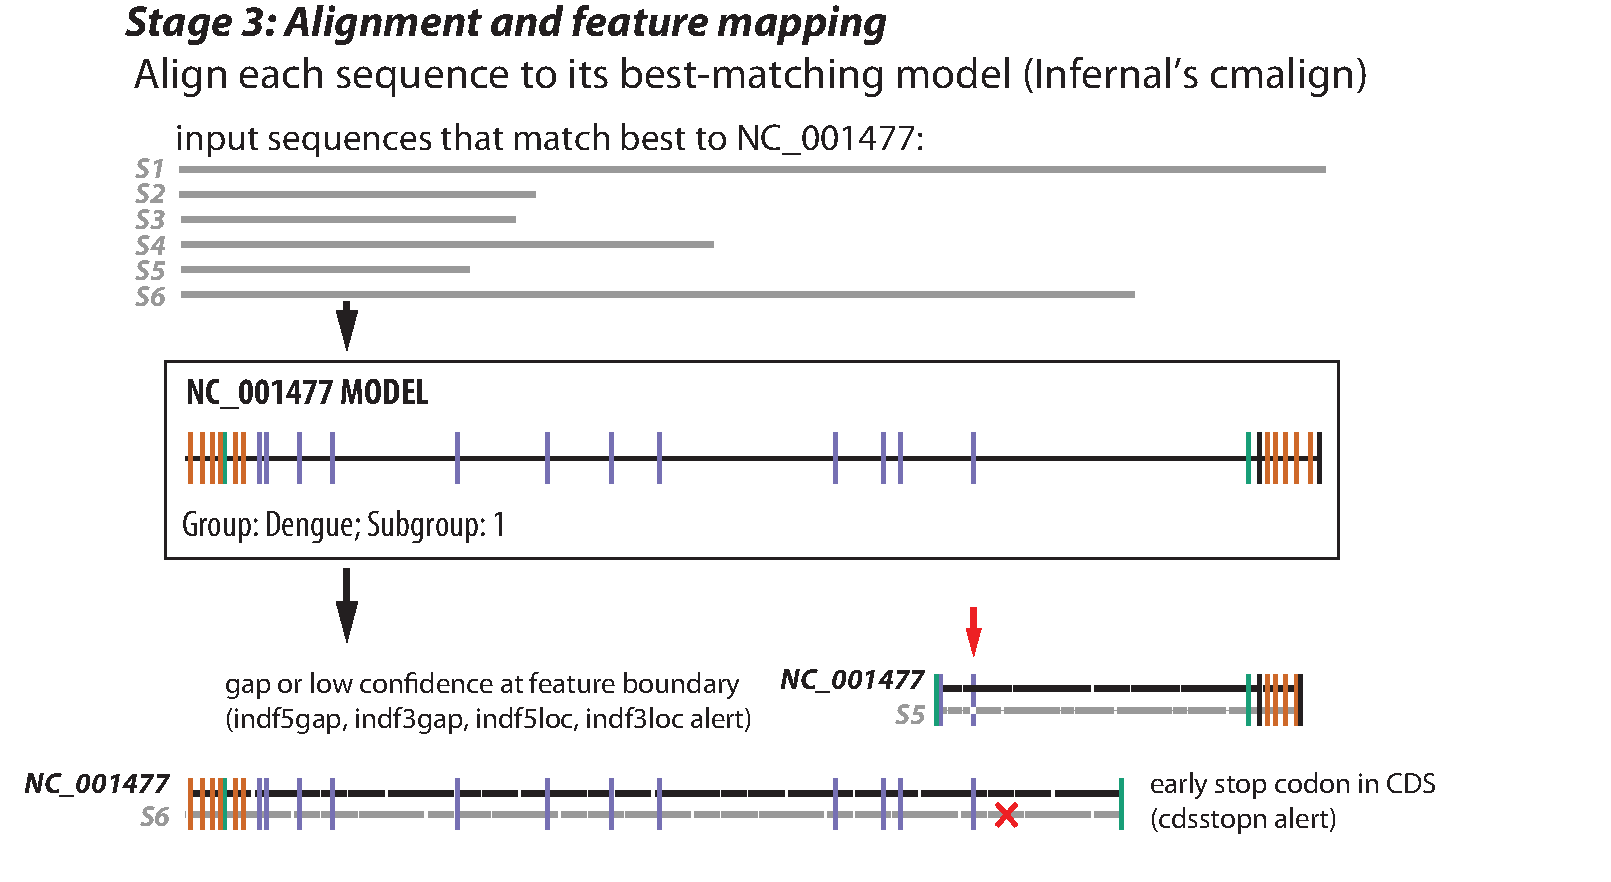
\includegraphics[width=10.5in]{figs/v-annotate-stage3-3}
%\end{center}
%
%\vfill
%\end{slide}
%%%%%%%%%%%%%%%%%%%%%%%%%%%%%%%%%%%%%%%%%%%%%%%%%%%%%%%%%%%%%%%%%%%%%%
\begin{slide}
\begin{center}

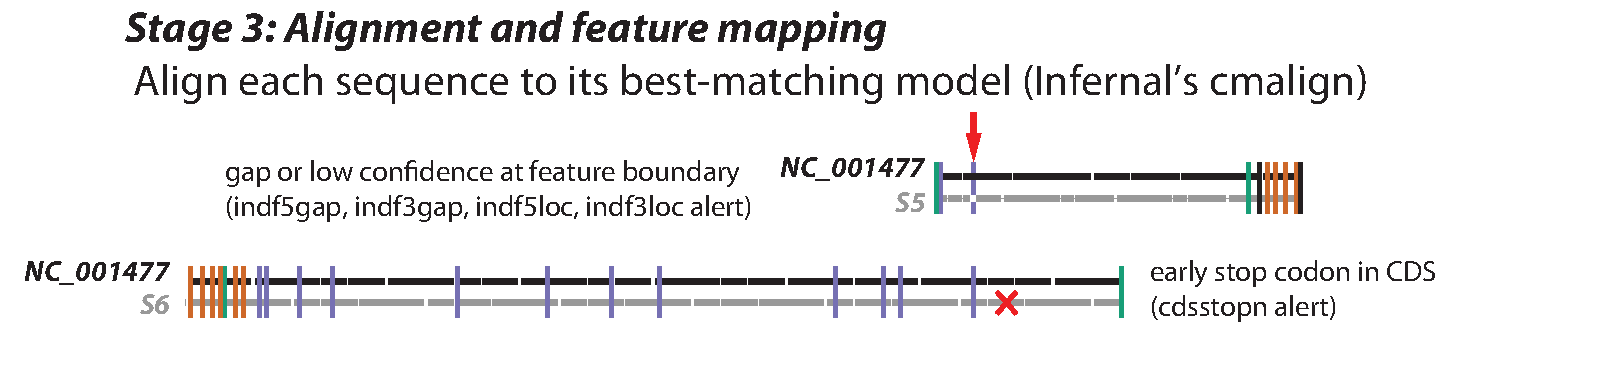
\includegraphics[width=10.5in]{figs/v-annotate-stage3-4}
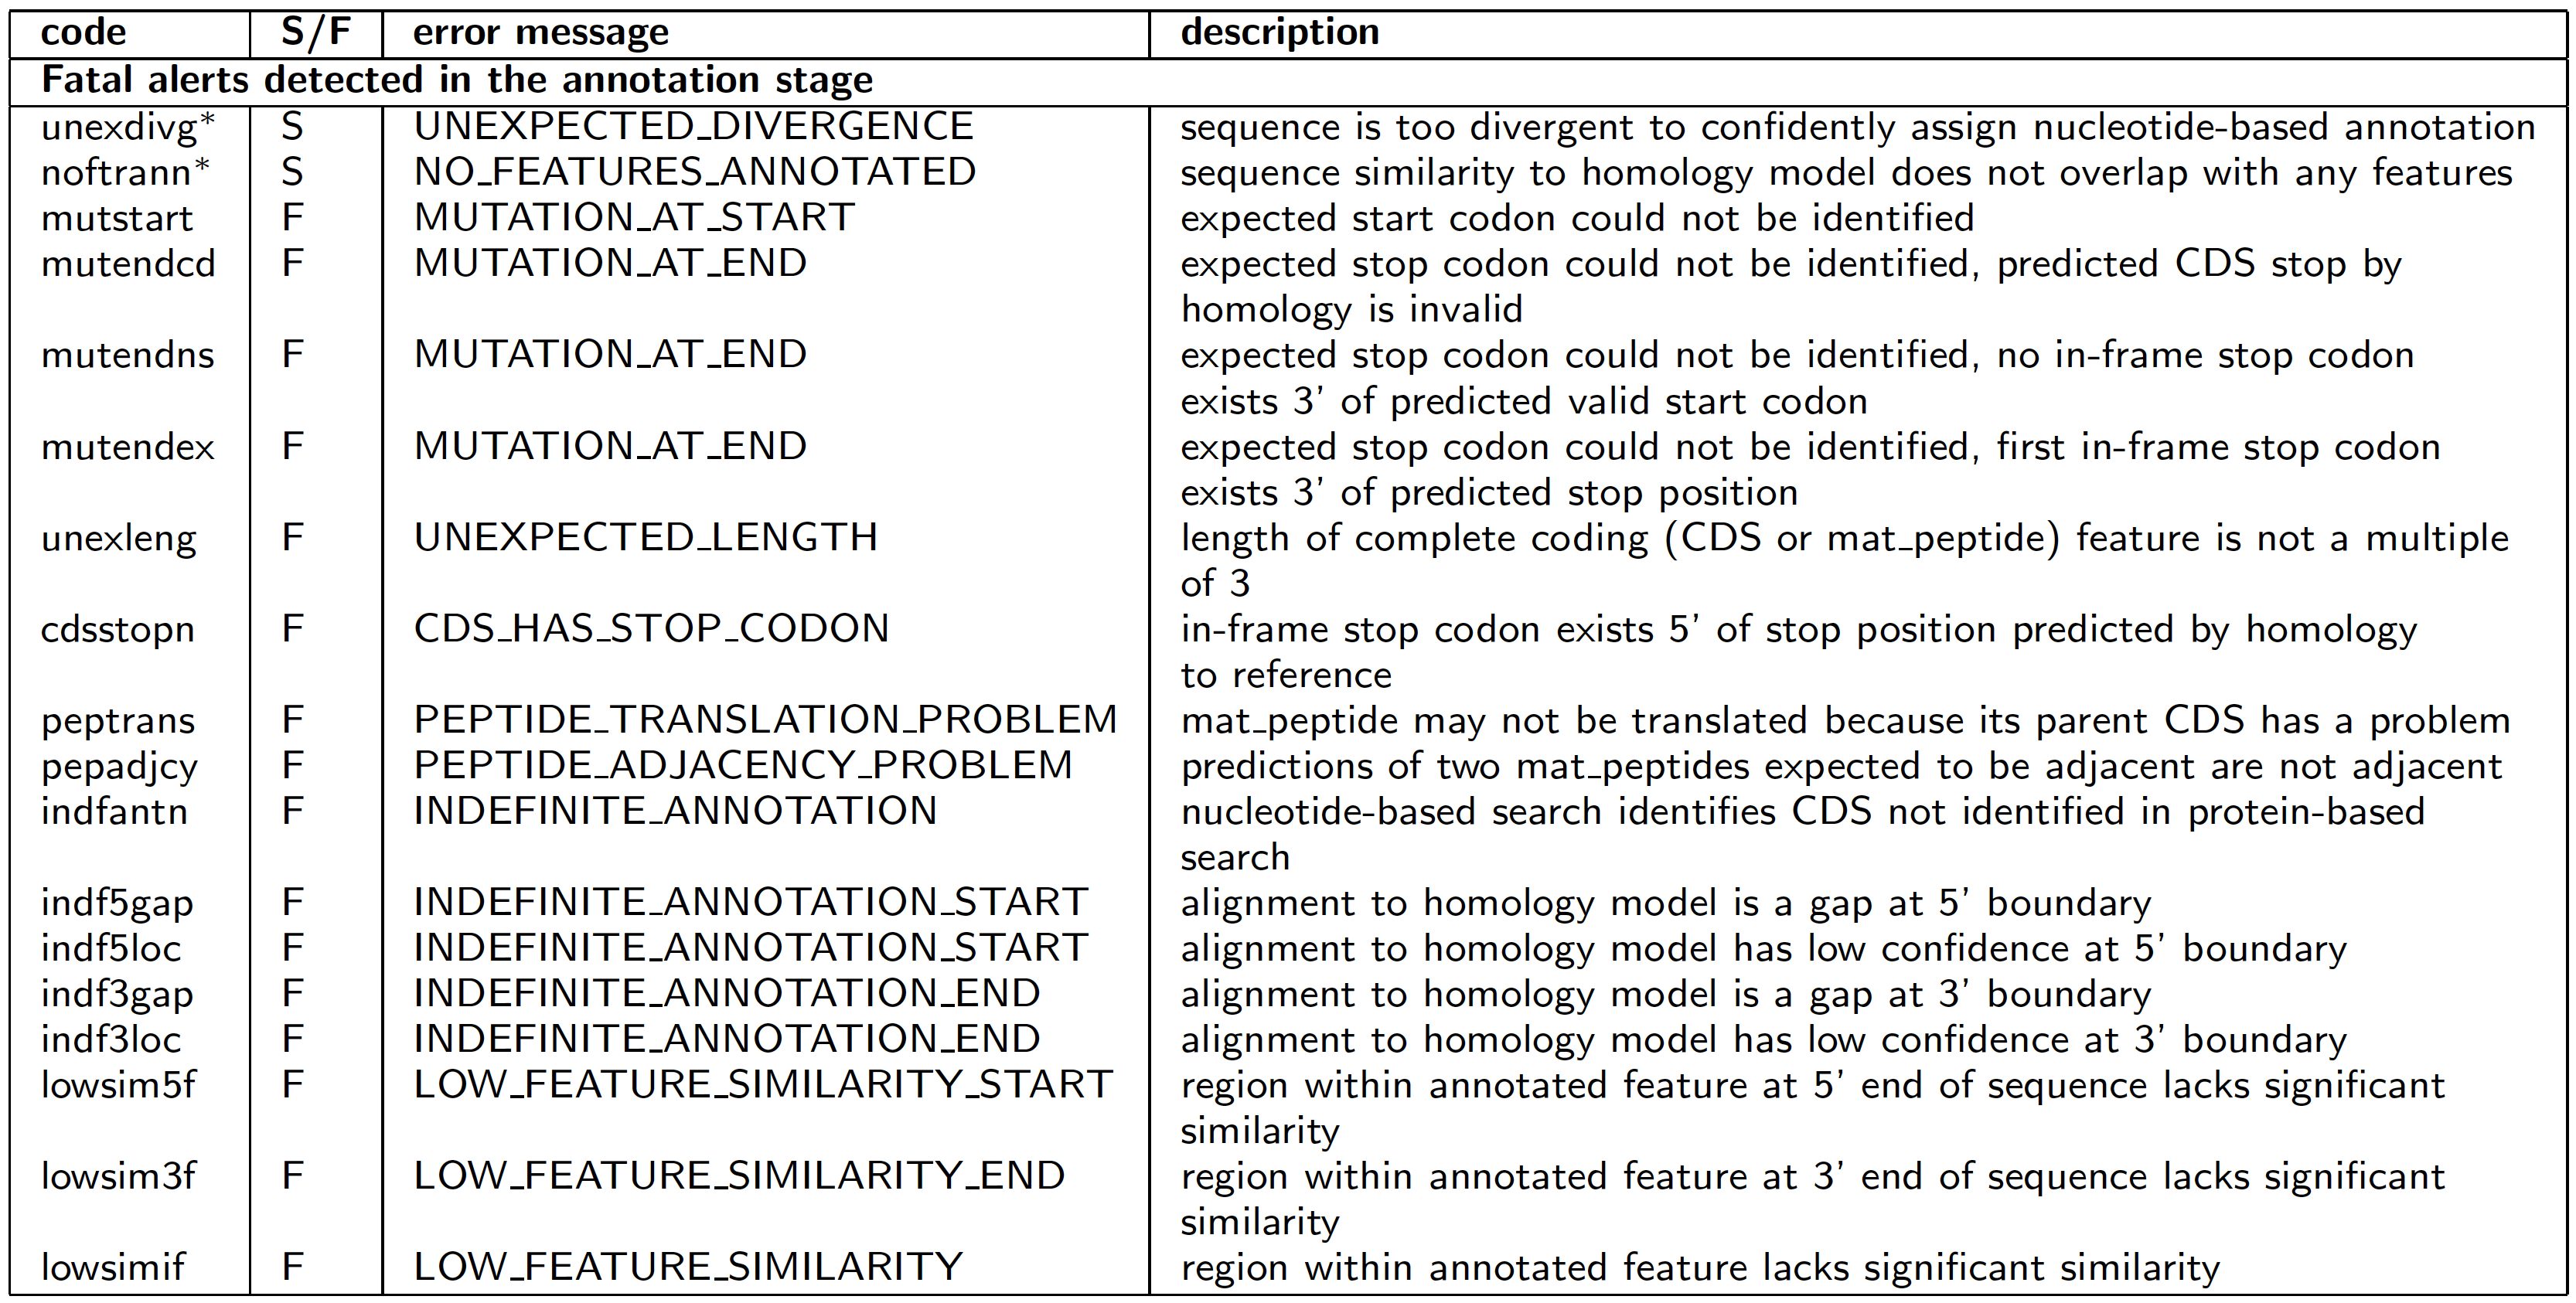
\includegraphics[width=10.5in]{figs/ss-alignment-alert-list}

\end{center}
\vfill
\end{slide}
%%%%%%%%%%%%%%%%%%%%%%%%%%%%%%%%%%%%%%%%%%%%%%%%%%%%%%%%%%%%%%%%%%%%%%
\begin{slide}
\begin{center}

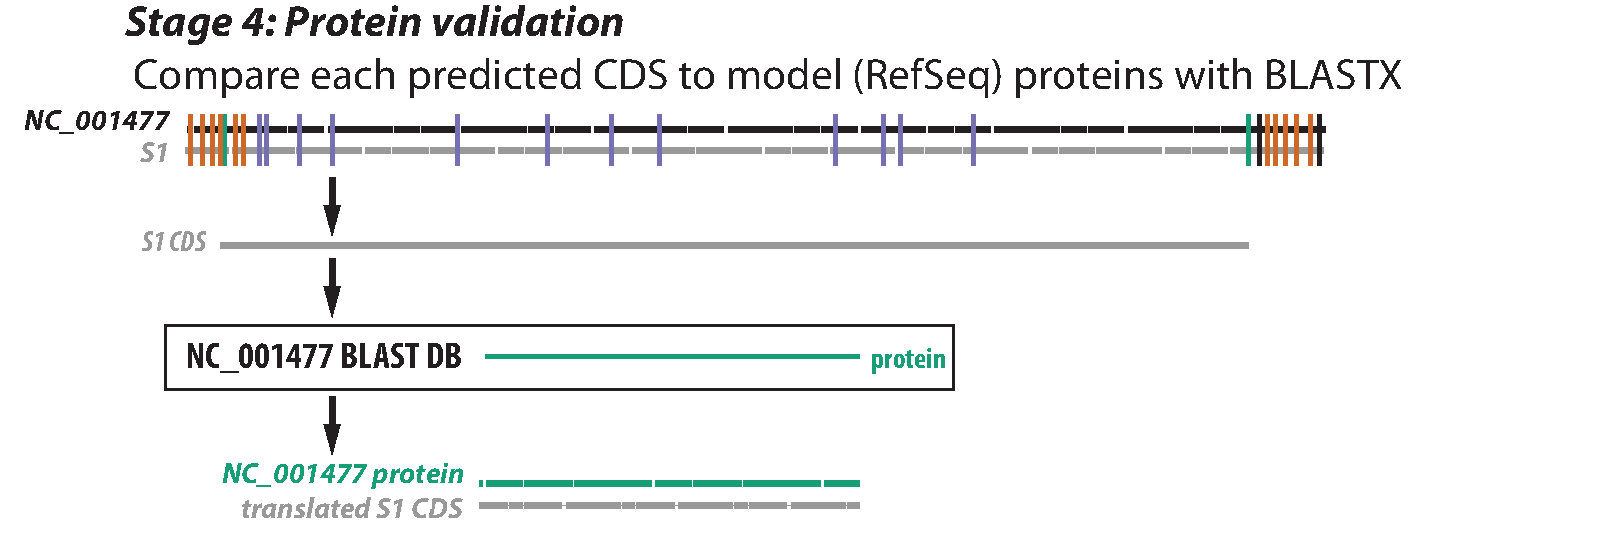
\includegraphics[width=10.5in]{figs/v-annotate-stage4-1}

\end{center}
\vfill
\end{slide}
%%%%%%%%%%%%%%%%%%%%%%%%%%%%%%%%%%%%%%%%%%%%%%%%%%%%%%%%%%%%%%%%%%%%%%
\begin{slide}
\begin{center}

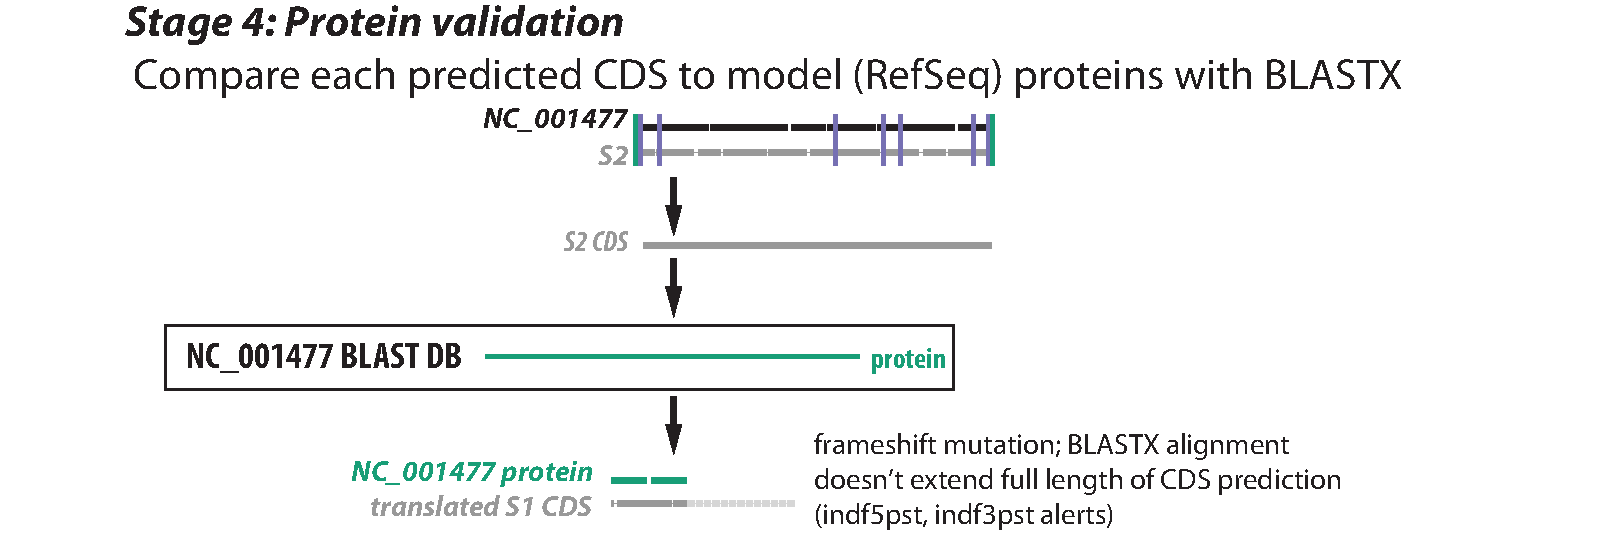
\includegraphics[width=10.5in]{figs/v-annotate-stage4-2}
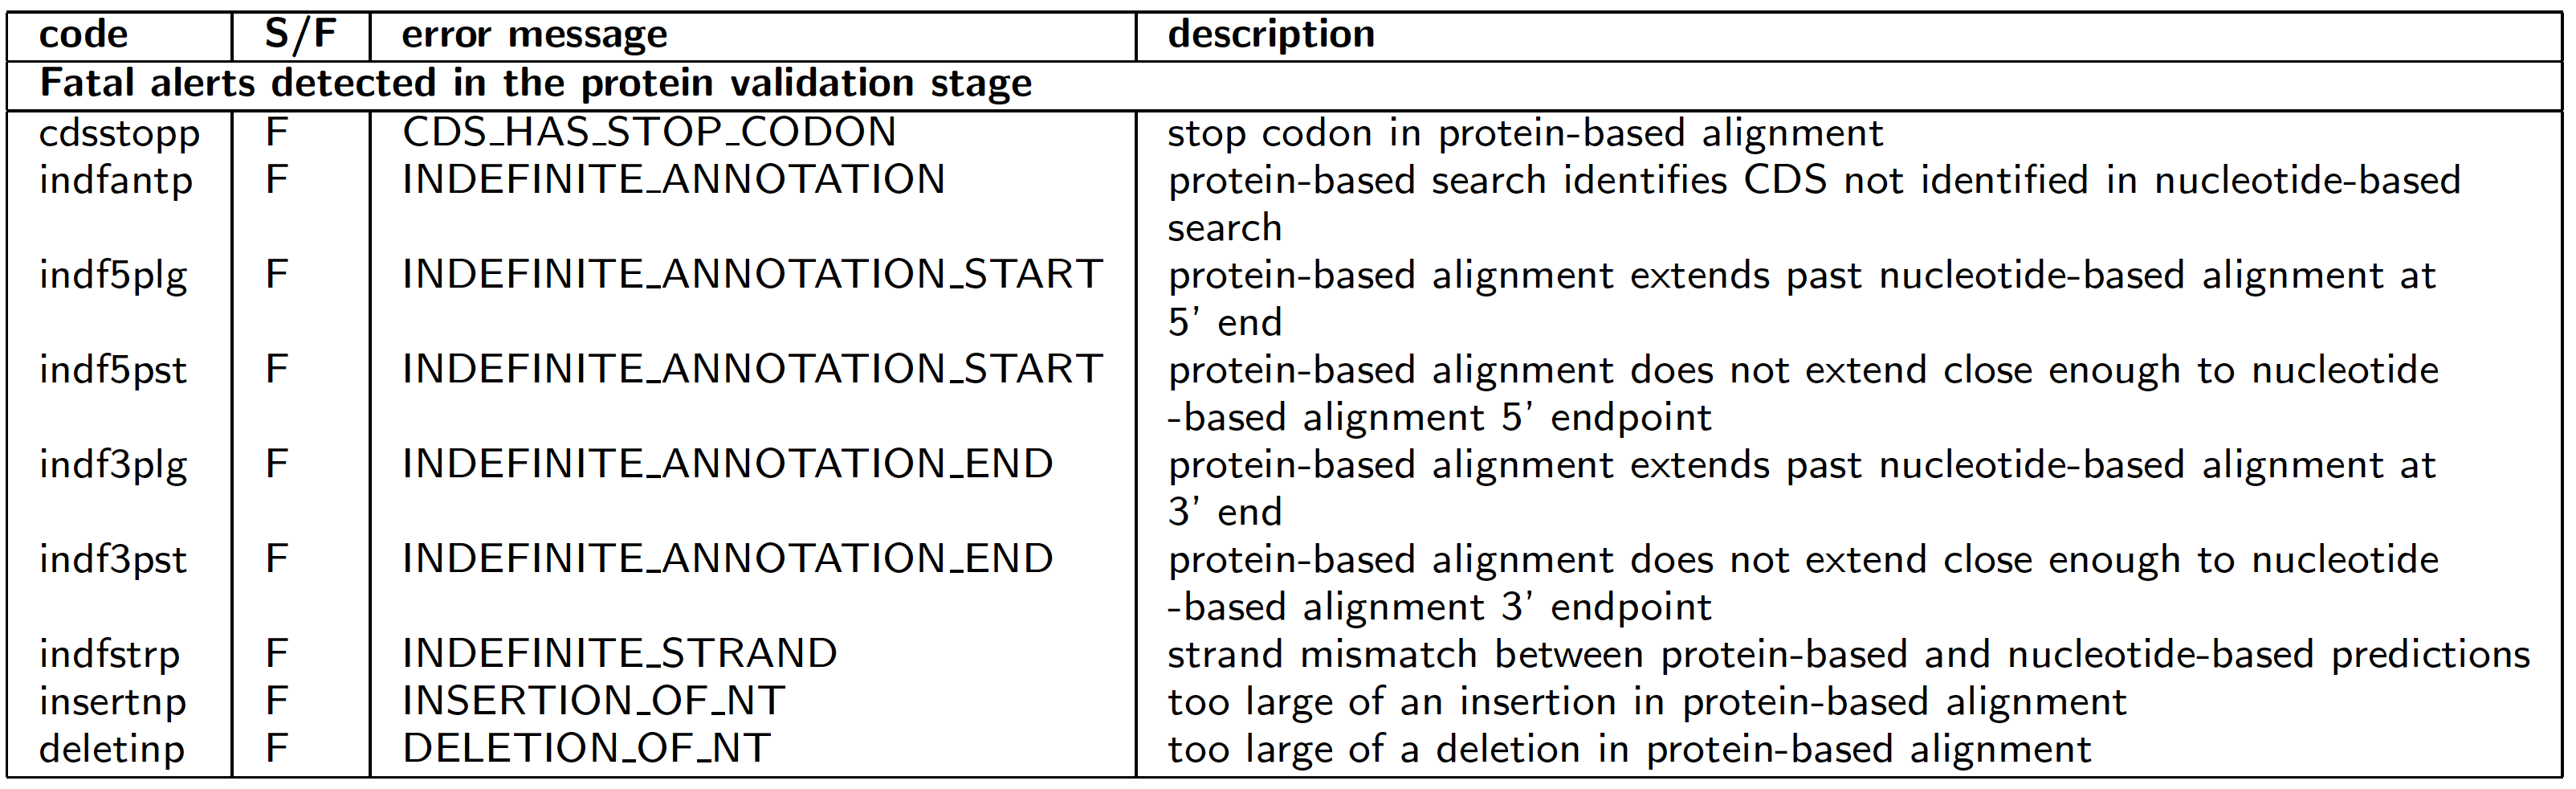
\includegraphics[width=10.5in]{figs/ss-protein-alert-list}

\end{center}
\vfill
\end{slide}
%%%%%%%%%%%%%%%%%%%%%%%%%%%%%%%%%%%%%%%%%%%%%%%%%%%%%%%%%%%%%%%%%%%%%%
\begin{slide}
\begin{center}
\textbf{VADR results on all Norovirus and Dengue sequences}


\scriptsize
\begin{tabular}{l|r|r|r|r|r|r}
                        &         & min    & max      &         &         & \textcolor{red}{fraction} \\
 dataset                & \# seqs & length & length   & \# pass & \# fail & \textcolor{red}{pass} \\ \hline
Norovirus complete (NC) & 1,384    & 7380  & 7839     & 1,157    & 227     & \textcolor{red}{0.836} \\
Dengue complete (DC)    & 4,580    & 10372 & 16254    & 4,171    & 409     & \textcolor{red}{0.911} \\
& & & & & \\
Norovirus partial (NP)  & 32,190   & 50    & 7376     & 29,488   & 2,702    & \textcolor{red}{0.916} \\
Dengue partial  (DP)    & 20,973   & 50    & 10370    & 17,276   & 3,697    & \textcolor{red}{0.824} \\
\end{tabular}

\end{center}
\vfill
\end{slide}
%%%%%%%%%%%%%%%%%%%%%%%%%%%%%%%%%%%%%%%%%%%%%%%%%%%%%%%%%%%%%%%%%%%%%%
\begin{slide}
\begin{center}
\textbf{VADR results on all Norovirus and Dengue sequences}


\scriptsize
\begin{tabular}{l|r|r|r|r|r|r}
                        &         & min    & max      &         &         & \textcolor{red}{fraction} \\
 dataset                & \# seqs & length & length   & \# pass & \# fail & \textcolor{red}{pass} \\ \hline
Norovirus complete (NC) & 1,384    & 7380  & 7839     & 1,157    & 227     & \textcolor{red}{0.836} \\
Dengue complete (DC)    & 4,580    & 10372 & 16254    & 4,171    & 409     & \textcolor{red}{0.911} \\
& & & & & \\
Norovirus partial (NP)  & 32,190   & 50    & 7376     & 29,488   & 2,702    & \textcolor{red}{0.916} \\
Dengue partial  (DP)    & 20,973   & 50    & 10370    & 17,276   & 3,697    & \textcolor{red}{0.824} \\
\end{tabular}

\medskip
\normalsize
\textbf{VADR is portable so submitters can run on their data prior to
  submission to save time}

\normalsize
\textbf{Sequences processed with VADR will include annotations of RNAs
  (\texttt{stem\_loop} and \texttt{ncRNA}) from models}

\end{center}
\vfill
\end{slide}
%%%%%%%%%%%%%%%%%%%%%%%%%%%%%%%%%%%%%%%%%%%%%%%%%%%%%%%%%%%%%%%%%%%%%%
%\begin{slide}
%\begin{center}
%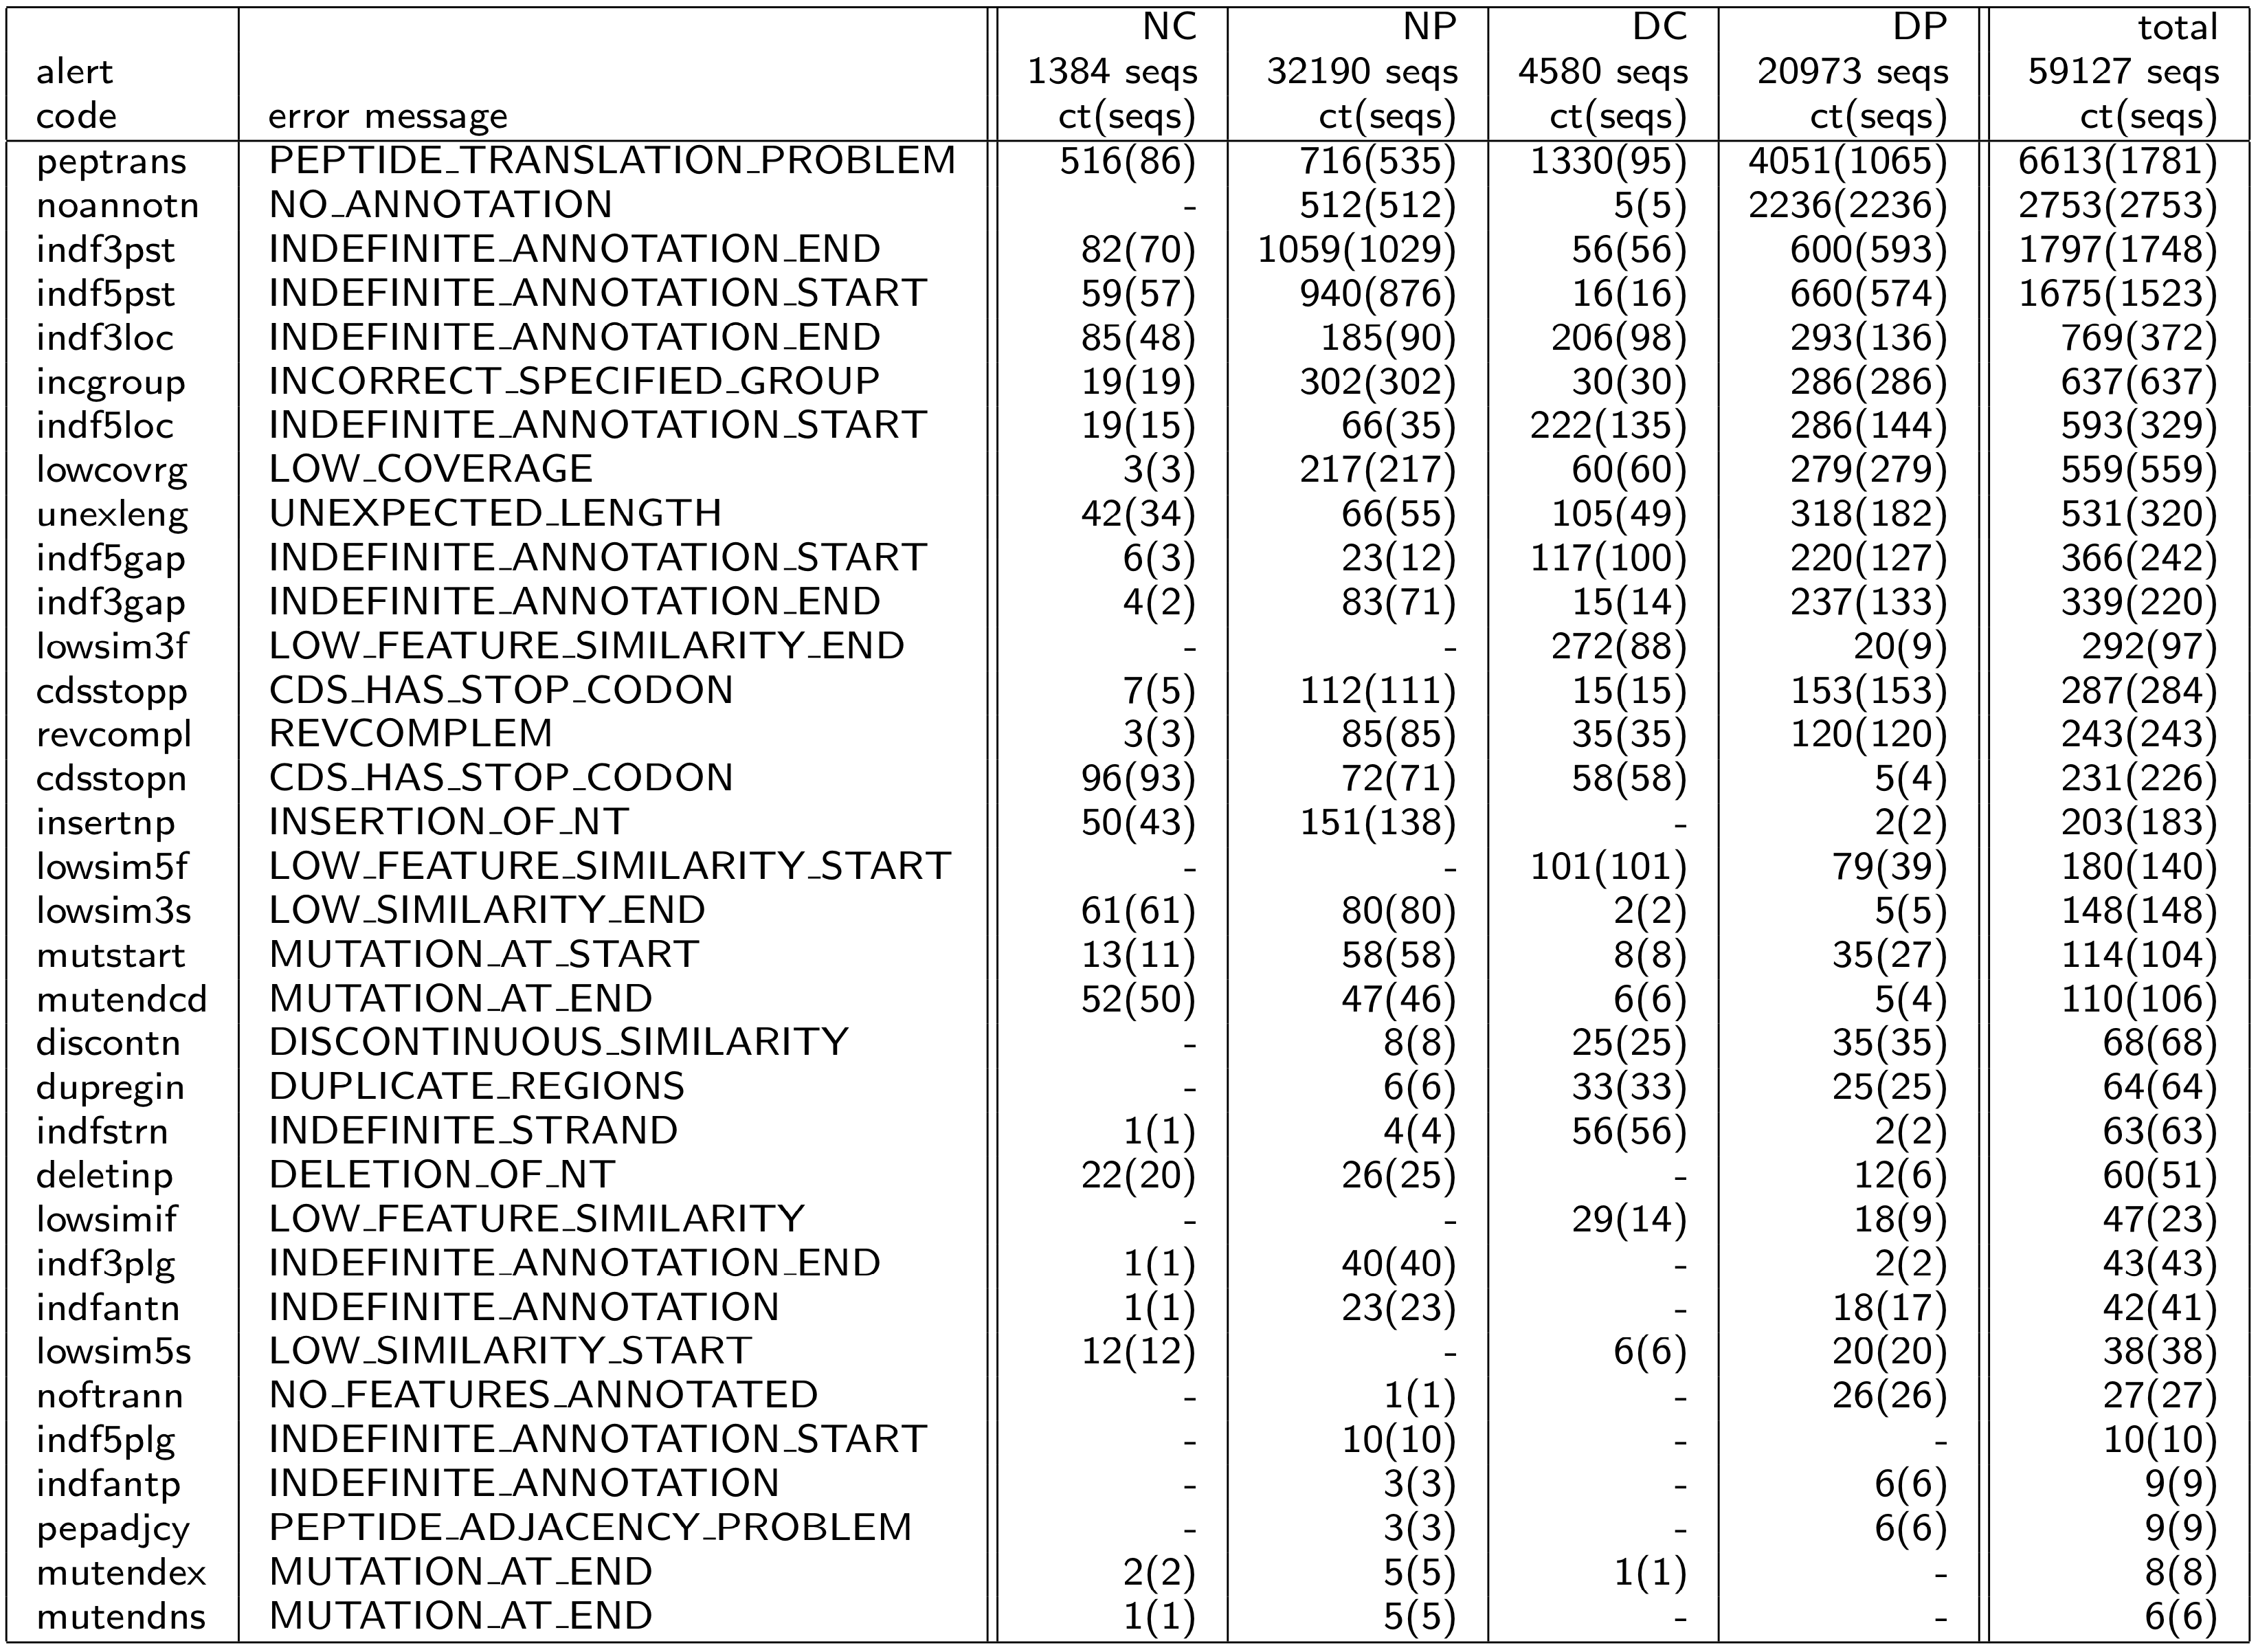
\includegraphics[width=10.5in]{figs/ss-alert-counts}
%\end{center}
%
%\vfill
%\end{slide}
%%%%%%%%%%%%%%%%%%%%%%%%%%%%%%%%%%%%%%%%%%%%%%%%%%%%%%%%%%%%%%%%%%%%%%
%\begin{slide}
%\begin{center}
%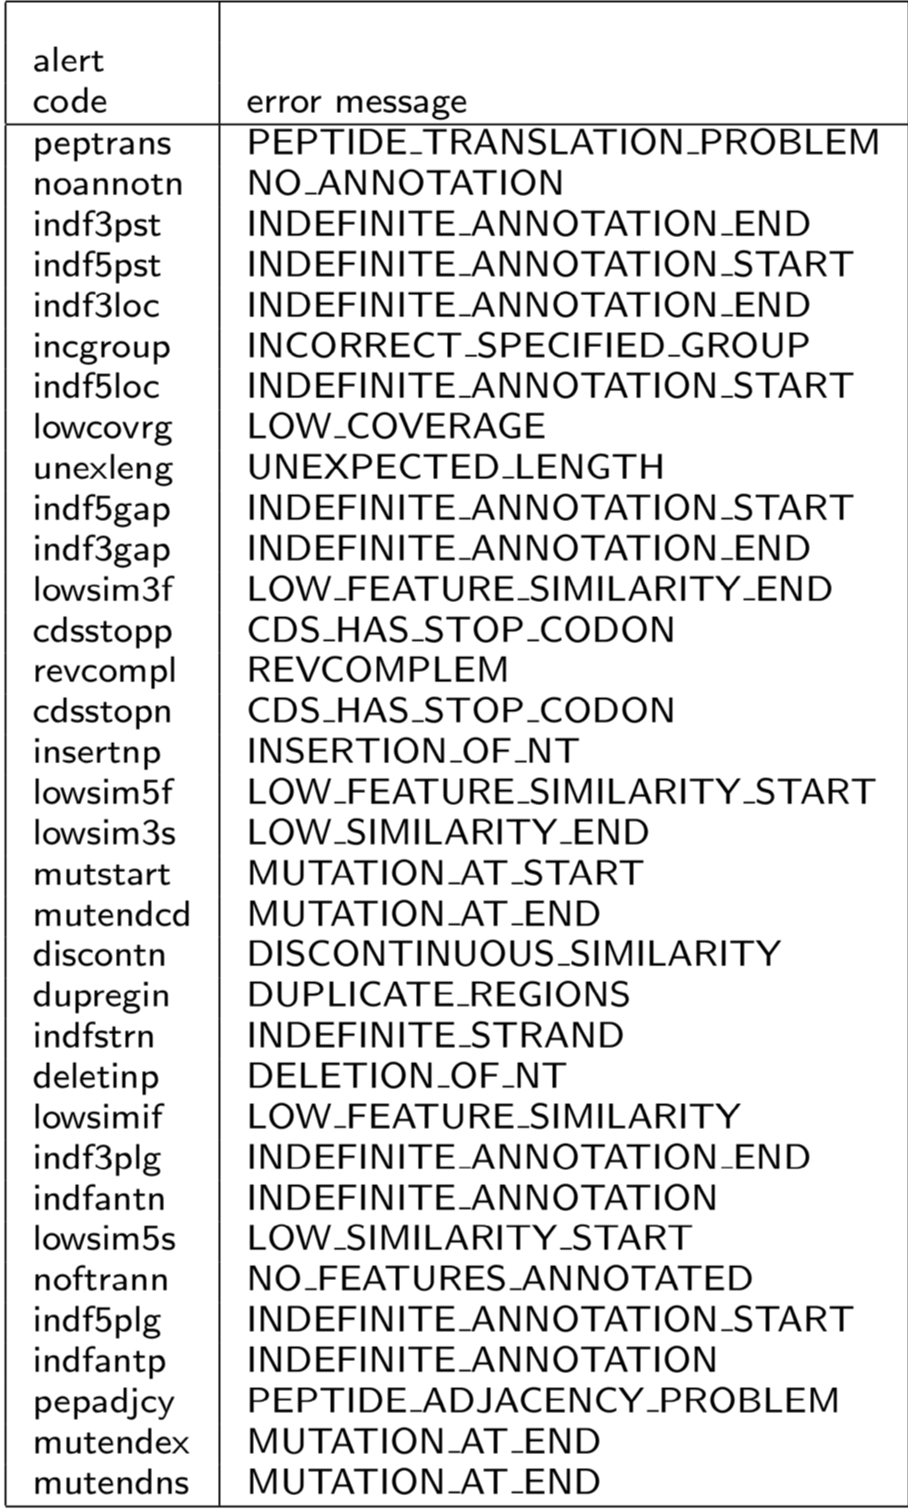
\includegraphics[height=8in]{figs/vadr-noro-dengue-ss-counts1}
%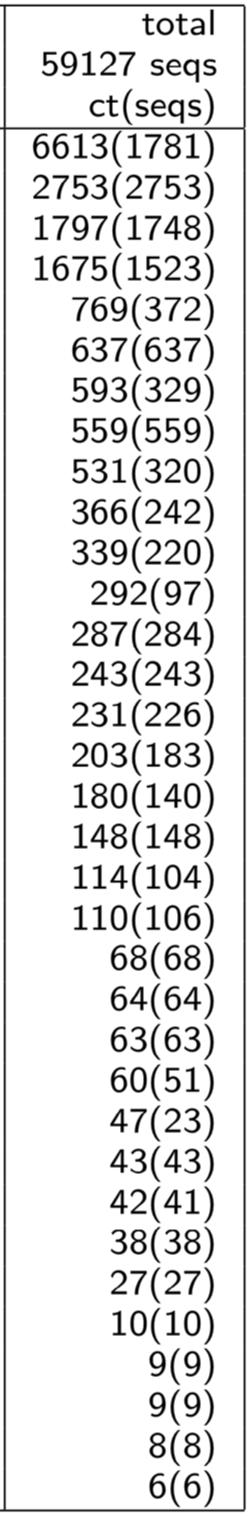
\includegraphics[height=8.02in]{figs/vadr-noro-dengue-ss-counts2}
%\end{center}
%
%\vfill
%\end{slide}
%%%%%%%%%%%%%%%%%%%%%%%%%%%%%%%%%%%%%%%%%%%%%%%%%%%%%%%%%%%%%%%%%%%%%%
\begin{slide}


\includegraphics[width=7in]{figs/blank-slide}
  
\vfill
\end{slide}
%%%%%%%%%%%%%%%%%%%%%%%%%%%%%%%%%%%%%%%%%%%%%%%%%%%%%%%%%%%%%%%%%%%%%%
\begin{slide}
\begin{center}
\normalsize{\textbf{SARS-CoV-2 sequence submissions in early 2020}}
\end{center}

\begin{center}
\begin{tabular}{llrr}
          &          &\#new     &\#cumulative\\
month     &year      &seqs      &seqs      \\ \hline
Jan       & 2020     &32        &32        \\ 
Feb       & 2020     &58        &90        \\ 
Mar       & 2020     &332       &422       \\ 
Apr       & 2020     &1541      &1963      \\ 
May       & 2020     &2974      &4937      \\ 
Jun       & 2020     &3394      &8331      \\ 
\end{tabular}
\end{center}

\vfill
\end{slide}
%%%%%%%%%%%%%%%%%%%%%%%%%%%%%%%%%%%%%%%%%%%%%%%%%%%%%%%%%%%%%%%%%%%%%%
\begin{slide}
\begin{center}
\normalsize{\textbf{SARS-CoV-2 sequence submissions have increased since early 2020}}
\end{center}

\tiny
\begin{center}
\begin{tabular}{llrr}
          &          &\#new     &\#cumulative\\
month     &year      &seqs      &seqs      \\ \hline
Jan       & 2020     &32        &32        \\ 
Feb       & 2020     &58        &90        \\ 
Mar       & 2020     &332       &422       \\ 
Apr       & 2020     &1541      &1963      \\ 
May       & 2020     &2974      &4937      \\ 
Jun       & 2020     &3394      &8331      \\ 
Jul       & 2020     &3604      &11,935    \\ 
Aug       & 2020     &3818      &15,753    \\ 
Sep       & 2020     &6731      &22,484    \\ 
Oct       & 2020     &11,939    &34,423    \\ 
Nov       & 2020     &4274      &38,697    \\ 
Dec       & 2020     &4530      &43,227    \\ 
& & & \\
Jan       & 2021     &8775      &52,002    \\ 
Feb       & 2021     &26,078    &78,080    \\ 
Mar       & 2021     &42,607    &120,687   \\ 
Apr       & 2021     &97,095    &217,782   \\ 
May       & 2021     &104,729   &322,511   \\ 
Jun       & 2021     &46,187    &368,698   \\ 
Jul       & 2021     &43,336    &412,034   \\ 
Aug       & 2021     &141,958   &553,992   \\ 
Sep       & 2021     &267,562   &821,554   \\ 
Oct       & 2021     &239,296   &1,060,850 \\ 
Nov       & 2021     &267,270   &1,328,120 \\ 
Dec       & 2021     &288,771   &1,616,891 \\ 
& & & \\
Jan       & 2022     &258,522   &1,875,413 \\ 
Feb       & 2022     &230,185   &2,105,598 \\ 
Mar       & 2022     &141,333   &2,246,931 \\ 
Apr       & 2022     &148,545   &2,395,476 \\
May       & 2022     &164,276   &2,559,752 \\
Jun       & 2022     &129,236   &2,688,988 \\
Jul       & 2022     &101,737   &2,790,725 \\
\end{tabular}
\end{center}

\vfill
\end{slide}
%%%%%%%%%%%%%%%%%%%%%%%%%%%%%%%%%%%%%%%%%%%%%%%%%%%%%%%%%%%%%%%%%%%%%%
\begin{slide}
\begin{center}
\normalsize{\textbf{SARS-CoV-2 sequences differ from Norovirus and Dengue virus \\ in several ways that impact VADR processing}}

\scriptsize
\begin{tabular}{r|r|r|r}
                                                  &Norovirus      &Dengue virus   &\textcolor{red}{SARS-CoV-2}      \\ \hline
length                                            &7.6Kb         &10.7Kb       &\textcolor{red}{29.9Kb}        \\
\# seqs                                           &44,936        &113,211         &\textcolor{red}{1,616,891}        \\
\% seqs full length                               &5.1\%          &8.4\%          &\textcolor{red}{99.7\%}         \\
\% Ns                                             &0.5\%          &0.2\%          &\textcolor{red}{1.4\%}          \\
\% seqs with stretch of $>=50$ Ns                 &1.0\%          &0.4\%          &\textcolor{red}{38.7\%}         \\
average \% identity                               &81.6\% &94.4\%         &\textcolor{red}{99.4\%}         \\ \hline
\multicolumn{4}{l}{} \\ 
\multicolumn{4}{l}{\textbf{VADR v1.0 performance}} \\ \hline
seconds per sequence                   &42.4           &92.6           &\textcolor{red}{331.8}          \\
required RAM                           &8Gb            &8Gb            &\textcolor{red}{64Gb}           \\
total running time, CPU days           &1.1            &10.2           &\textcolor{red}{6187.6}         \\
\end{tabular}
\end{center}

\vfill
\end{slide}
%%%%%%%%%%%%%%%%%%%%%%%%%%%%%%%%%%%%%%%%%%%%%%%%%%%%%%%%%%%%%%%%%%%%%%
\begin{slide}
\begin{center}
\normalsize{\textbf{SARS-CoV-2 sequences differ from Norovirus and Dengue virus \\ in several ways that impact VADR processing}}

\scriptsize
\begin{tabular}{r|r|r|r}
                                                  &Norovirus      &Dengue virus   &\textcolor{red}{SARS-CoV-2}      \\ \hline
length                                            &7.6Kb         &10.7Kb       &\textcolor{red}{29.9Kb}        \\
\# seqs                                           &44,936        &113,211         &\textcolor{red}{1,616,891}        \\
\% seqs full length                               &5.1\%          &8.4\%          &\textcolor{red}{99.7\%}         \\
\% Ns                                             &0.5\%          &0.2\%          &\textcolor{red}{1.4\%}          \\
\% seqs with stretch of $>=50$ Ns                 &1.0\%          &0.4\%          &\textcolor{red}{38.7\%}         \\
average \% identity                               &81.6\% &94.4\%         &\textcolor{red}{99.4\%}         \\ \hline
\multicolumn{4}{l}{} \\ 
\multicolumn{4}{l}{\textbf{VADR v1.0 performance}} \\ \hline
seconds per sequence                   &42.4           &92.6           &\textcolor{red}{331.8}          \\
required RAM                           &8Gb            &8Gb            &\textcolor{red}{64Gb}           \\
total running time, CPU days           &1.1            &10.2           &\textcolor{red}{6187.6}         \\
\end{tabular}
\end{center}

\begin{itemize}
  \item CDC expected large increase in sequence data submissions
  \item Needed to quickly accelerate SARS-CoV-2 annotation
  \item \emph{WARNING: brutal hacks implemented and explained next}
\end{itemize}  

\vfill
\end{slide}
%%%%%%%%%%%%%%%%%%%%%%%%%%%%%%%%%%%%%%%%%%%%%%%%%%%%%%%%%%%%%%%%%%%%%%
\begin{slide}
\begin{center}
\normalsize{\textbf{Replacing Ns with expected nucleotides allows \\ many 'good' sequences to pass}}

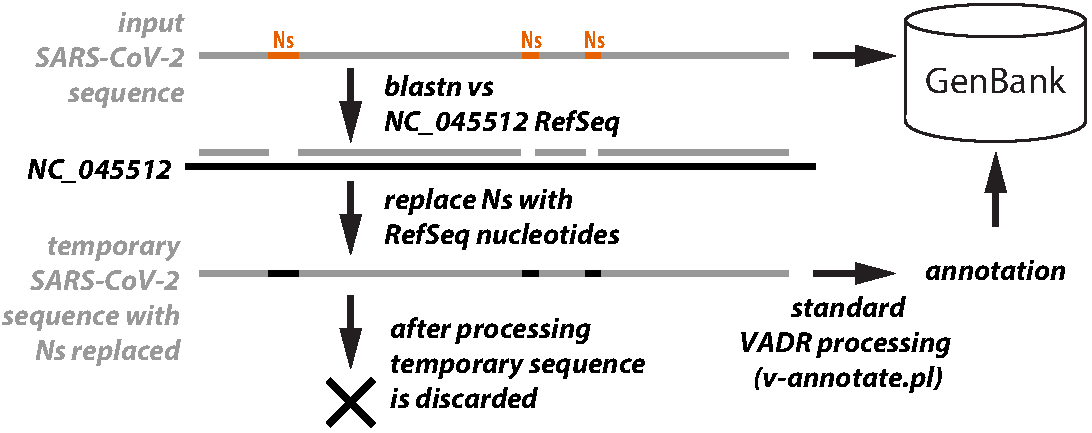
\includegraphics[width=10.25in]{figs/vadr-r-option}
\end{center}

\vfill
\end{slide}
%%%%%%%%%%%%%%%%%%%%%%%%%%%%%%%%%%%%%%%%%%%%%%%%%%%%%%%%%%%%%%%%%%%%%%
\begin{slide}
\begin{center}
\normalsize{\textbf{Seeded alignment using blastn makes alignment stage faster}}

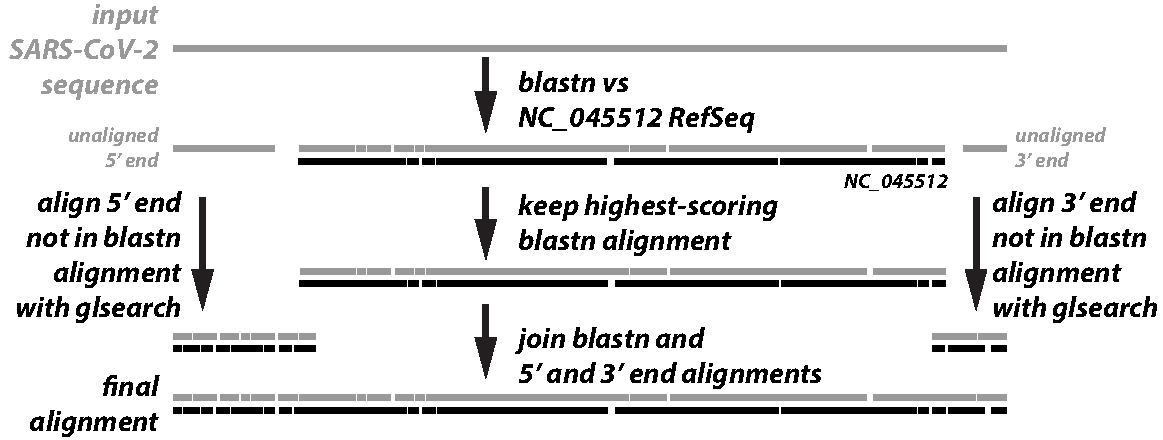
\includegraphics[width=10.25in]{figs/vadr-s-option}
\end{center}

\vfill
\end{slide}
%%%%%%%%%%%%%%%%%%%%%%%%%%%%%%%%%%%%%%%%%%%%%%%%%%%%%%%%%%%%%%%%%%%%%%
\begin{slide}
\begin{center}
\textbf{Using glsearch instead of cmalign reduces memory requirement}
\end{center}

\begin{itemize}
\item lower memory requirement (2Gb max) allows for multi-threading
%  \item input file is split into chunks
%    \begin{itemize}
%    \item each chunk processed independently in parallel on one of 8 CPUs
%    \item further reduces memory requirement for large input files \\ (dependent on chunk size
%      instead of input file size)
%    \end{itemize}
\end{itemize}

\begin{center}
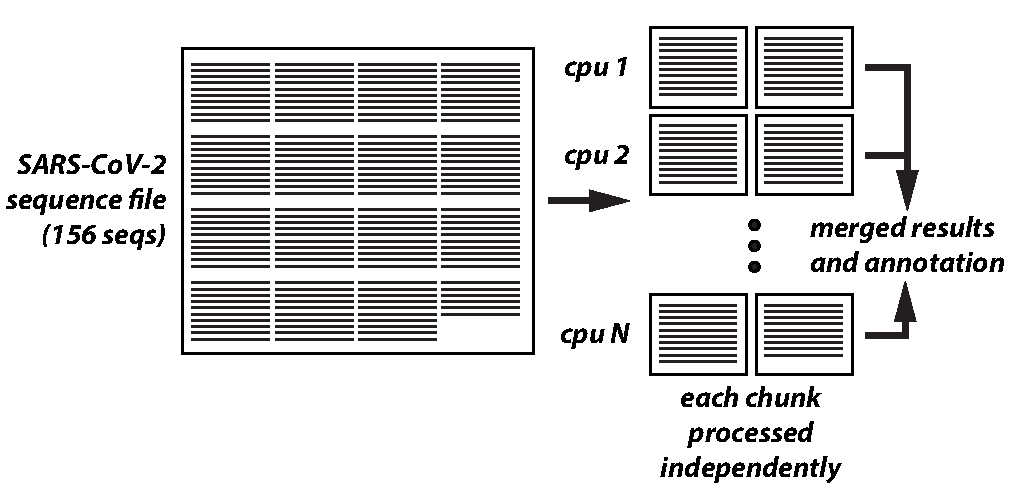
\includegraphics[width=10.5in]{figs/vadr-1p2-multithreading}
\end{center}
  
\vfill
\end{slide}
%%%%%%%%%%%%%%%%%%%%%%%%%%%%%%%%%%%%%%%%%%%%%%%%%%%%%%%%%%%%%%%%%%%%%%
\begin{slide}
\begin{center}
\normalsize{\textbf{VADR is now 1000-fold faster in practice for SARS-CoV-2 processing}}

\scriptsize
\begin{tabular}{lrrrrrrrr}
            &seeded      &N           &            &            &            &secs        &hours       &speedup     \\ 
VADR        &align-      &replace-    &            &\#          &required    &per         &per 100K    &vs          \\ 
version     &ment?       &ment?       &glsearch?   &cpus        &RAM         &seq         &seqs        &v1.0        \\ 
\hline
& & & & & & & & \\
v1.0        &$-$         &$-$         &$-$         &1           &64 Gb       &329.91      &9164.3      &-           \\
\end{tabular}
\end{center}

\vfill
\end{slide}
%%%%%%%%%%%%%%%%%%%%%%%%%%%%%%%%%%%%%%%%%%%%%%%%%%%%%%%%%%%%%%%%%%%%%%
\begin{slide}
\begin{center}
\normalsize{\textbf{VADR is now 1000-fold faster in practice for SARS-CoV-2 processing}}

\scriptsize
\begin{tabular}{lrrrrrrrr}
            &seeded      &N           &            &            &            &secs        &hours       &speedup     \\ 
VADR        &align-      &replace-    &            &\#          &required    &per         &per 100K    &vs          \\ 
version     &ment?       &ment?       &glsearch?   &cpus        &RAM         &seq         &seqs        &v1.0        \\ 
\hline
& & & & & & & & \\
v1.0         &$-$         &$-$         &$-$         &1           &64 Gb       &329.91      &9164.3      &-           \\
%1.1         &$+$         &$+$         &$-$         &1           &64 Gb       &49.35       &1370.7      &6.7         \\
& & & & & & & & \\
v1.4.1       &$+$         &$+$         &$+$         &1           &2 Gb        &2.51        &69.8        &131.4       \\
\end{tabular}
\end{center}

\vfill
\end{slide}
%%%%%%%%%%%%%%%%%%%%%%%%%%%%%%%%%%%%%%%%%%%%%%%%%%%%%%%%%%%%%%%%%%%%%%
\begin{slide}
\begin{center}
\normalsize{\textbf{VADR is now 1000-fold faster in practice for SARS-CoV-2 processing}}

\scriptsize
\begin{tabular}{lrrrrrrrr}
            &seeded      &N           &            &            &            &secs        &hours       &speedup     \\ 
VADR        &align-      &replace-    &            &\#          &required    &per         &per 100K    &vs          \\ 
version     &ment?       &ment?       &glsearch?   &cpus        &RAM         &seq         &seqs        &v1.0        \\ 
\hline
& & & & & & & & \\
v1.0         &$-$         &$-$         &$-$         &1           &64 Gb       &329.91      &9164.3      &-           \\
%v1.1         &$+$         &$+$         &$-$         &1           &64 Gb       &49.35       &1370.7      &6.7         \\
& & & & & & & & \\
v1.4.1       &$+$         &$+$         &$+$         &1           &2 Gb        &2.51        &69.8        &131.4       \\
& & & & & & & & \\
%v1.4.1       &$+$         &$+$         &$+$         &2           &4 Gb        &1.49        &41.5        &220.8       \\
%& & & & & & & & \\
%v1.4.1       &$+$         &$+$         &$+$         &4           &8 Gb        &0.65        &18.0        &509.9       \\
%& & & & & & & & \\
\textbf{v1.4.1}&\textbf{$+$}&\textbf{$+$}&\textbf{$+$}&\textbf{8}  &\textbf{16 Gb}&\textbf{0.33}&\textbf{9.3}&\textbf{986.8}\\
& & & & & & & & \\
%v1.4.1       &$+$         &$+$         &$+$         &16          &32 Gb       &0.23        &6.5         &1417.9      \\
%& & & & & & & & \\
v1.4.1       &$+$         &$+$         &$+$         &32          &64 Gb       &0.13        &3.7         &2462.2      \\
\end{tabular}
\end{center}

\vfill
\end{slide}
%%%%%%%%%%%%%%%%%%%%%%%%%%%%%%%%%%%%%%%%%%%%%%%%%%%%%%%%%%%%%%%%%%%%%%
\begin{slide}
\begin{center}
\normalsize{\textbf{VADR is now fast enough to handle \\ hundreds of thousands of sequences per month}}
\end{center}

\tiny
\begin{center}
\begin{tabular}{llrr}
          &          &\#new     &\#cumulative\\
month     &year      &seqs      &seqs      \\ \hline
Jan       & 2020     &32        &32        \\ 
Feb       & 2020     &58        &90        \\ 
Mar       & 2020     &332       &422       \\ 
Apr       & 2020     &1541      &1963      \\ 
May       & 2020     &2974      &4937      \\ 
Jun       & 2020     &3394      &8331      \\ 
Jul       & 2020     &3604      &11,935    \\ 
Aug       & 2020     &3818      &15,753    \\ 
Sep       & 2020     &6731      &22,484    \\ 
Oct       & 2020     &11,939    &34,423    \\ 
Nov       & 2020     &4274      &38,697    \\ 
Dec       & 2020     &4530      &43,227    \\ 
& & & \\
Jan       & 2021     &8775      &52,002    \\ 
Feb       & 2021     &26,078    &78,080    \\ 
Mar       & 2021     &42,607    &120,687   \\ 
Apr       & 2021     &97,095    &217,782   \\ 
May       & 2021     &104,729   &322,511   \\ 
Jun       & 2021     &46,187    &368,698   \\ 
Jul       & 2021     &43,336    &412,034   \\ 
Aug       & 2021     &141,958   &553,992   \\ 
Sep       & 2021     &267,562   &821,554   \\ 
Oct       & 2021     &239,296   &1,060,850 \\ 
Nov       & 2021     &267,270   &1,328,120 \\ 
Dec       & 2021     &288,771   &1,616,891 \\ 
& & & \\
Jan       & 2022     &258,522   &1,875,413 \\ 
Feb       & 2022     &230,185   &2,105,598 \\ 
Mar       & 2022     &141,333   &2,246,931 \\ 
Apr       & 2022     &148,545   &2,395,476 \\
May       & 2022     &164,276   &2,559,752 \\
Jun       & 2022     &129,236   &2,688,988 \\
Jul       & 2022     &101,737   &2,790,725 \\
\end{tabular}
\end{center}

\vfill
\end{slide}
%%%%%%%%%%%%%%%%%%%%%%%%%%%%%%%%%%%%%%%%%%%%%%%%%%%%%%%%%%%%%%%%%%%%%%
\begin{slide}
\begin{center}
\textbf{Besides getting faster, VADR has changed in other ways \\ (work with Linda Yankie and Vince Calhoun and GenBank team)}

\begin{itemize}
\item 14 releases since March 2020 (thanks to ``git flow''\footnote{https://nvie.com/posts/a-successful-git-branching-model/})
\item 3 additional SARS-CoV-2 models (all eventually dropped):
  \begin{itemize}
  \item B.1.1.7 (alpha)
  \item B.1.525
  \item 28254-deletion
  \end{itemize}
\item allow some alerts for non-essential ORFs and s2m RNA element \\ without failing sequence (they become a \texttt{misc\_feature} instead)
\end{itemize}

\end{center}

\vfill
\end{slide}
% cut comparison to vigor and vapid
%%%%%%%%%%%%%%%%%%%%%%%%%%%%%%%%%%%%%%%%%%%%%%%%%%%%%%%%%%%%%%%%%%%%%%
\begin{slide}
\begin{center}
\textbf{VADR is a general tool}
\end{center}

\small
\begin{itemize}
\item Also used for COX1 (cytochrome C oxidase subunit I) sequences
  using 43 class or order specific \emph{profile}-based models
  covering 5 genetic codes
\end{itemize}

\normalsize
\begin{center}
  \textbf{Limitations}
\end{center}

\small
\begin{itemize}
\item nucleotide space, not protein space
\item RefSeq or alignment must be 'representative' and conserved along
  full length
  \begin{itemize}
    \item divergent sequences, regions, repeats, introns, gene order are problematic
  \end{itemize}
\item slow
\end{itemize}

%\normalsize
%\begin{center}
%  \textbf{Future directions}
%\end{center}

%\small
%\begin{itemize}
%\item extend to more viruses
%\item alignment-based models for viruses (testing with HCV)
%\end{itemize}

\vfill
\end{slide}
%%%%%%%%%%%%%%%%%%%%%%%%%%%%%%%%%%%%%%%%%%%%%%%%%%%%%%%%%%%%%%%%%%%%%
%\textbf{Future directions}
%\end{center}
%
%\small
%\begin{itemize}
%\item alignment-based models for viruses (testing with HCV)
%\item profile-based protein validation to replace BLASTX (HMMER)
%\item allow scanning of large sequences (e.g. genomes)
%\item extend to more genes, including ribosomal RNAs and possible ITS
%  sequences 
%\end{itemize}
%
%\vfill
%\end{slide}
%%%%%%%%%%%%%%%%%%%%%%%%%%%%%%%%%%%%%%%%%%%%%%%%%%%%%%%%%%%%%%%%%%%%%%%
\begin{slide}
\begin{center}

\includegraphics[width=6in]{figs/ribovore-paper-title}
%\textbf{Ribovore: ribosomal RNA sequence analysis for GenBank}

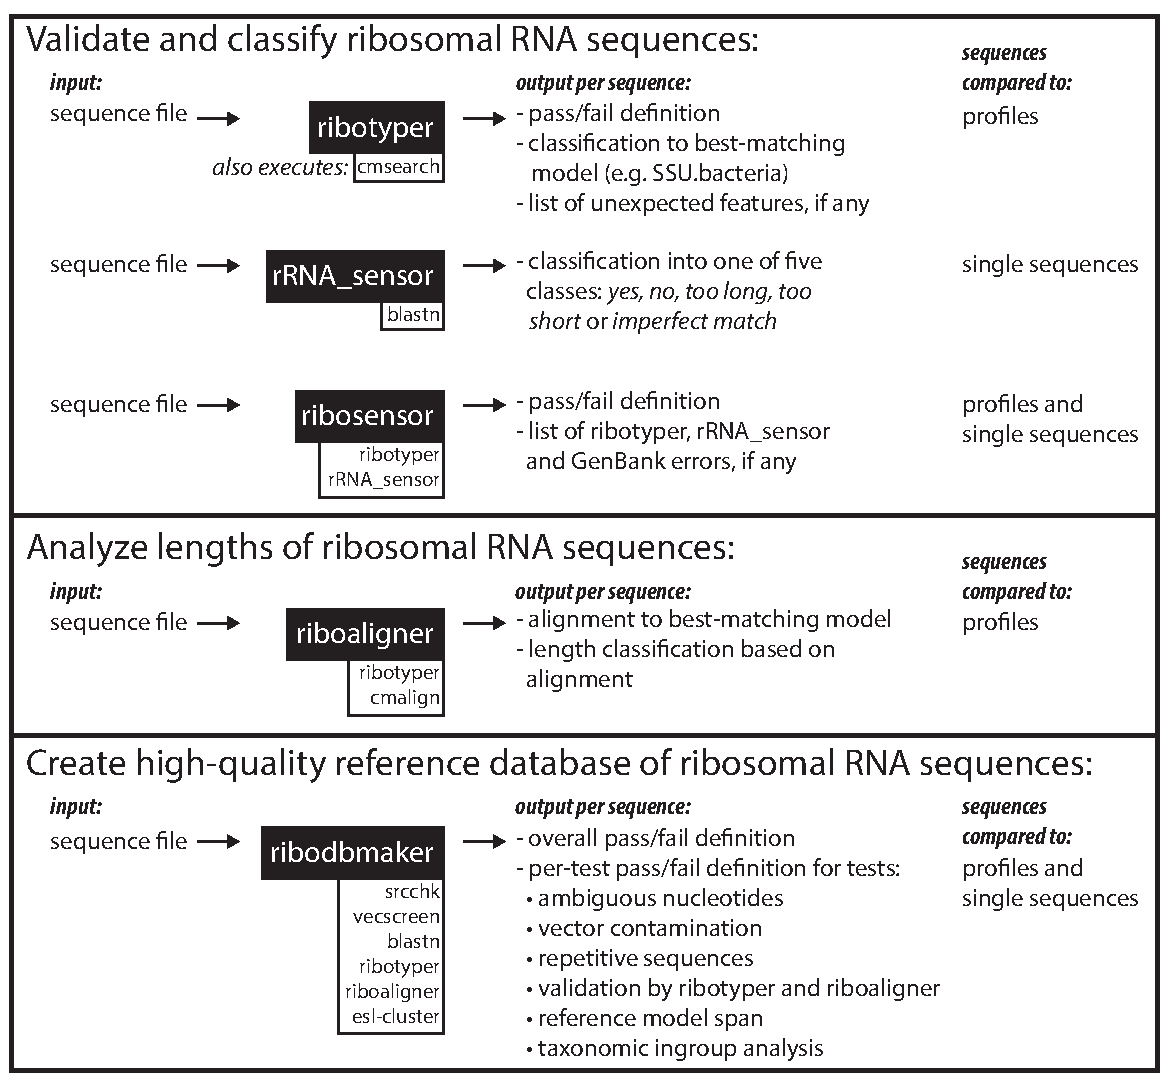
\includegraphics[height=5in]{figs/ribovore}
\end{center}

\vfill
\end{slide}
%%%%%%%%%%%%%%%%%%%%%%%%%%%%%%%%%%%%%%%%%%%%%%%%%%%%%%%%%%%%%%%%%%%%%%
\begin{slide}
\begin{center}
\textbf{Ribovore will (hopefully) help drive addition \\ and improvement of
  Rfam rRNA models}

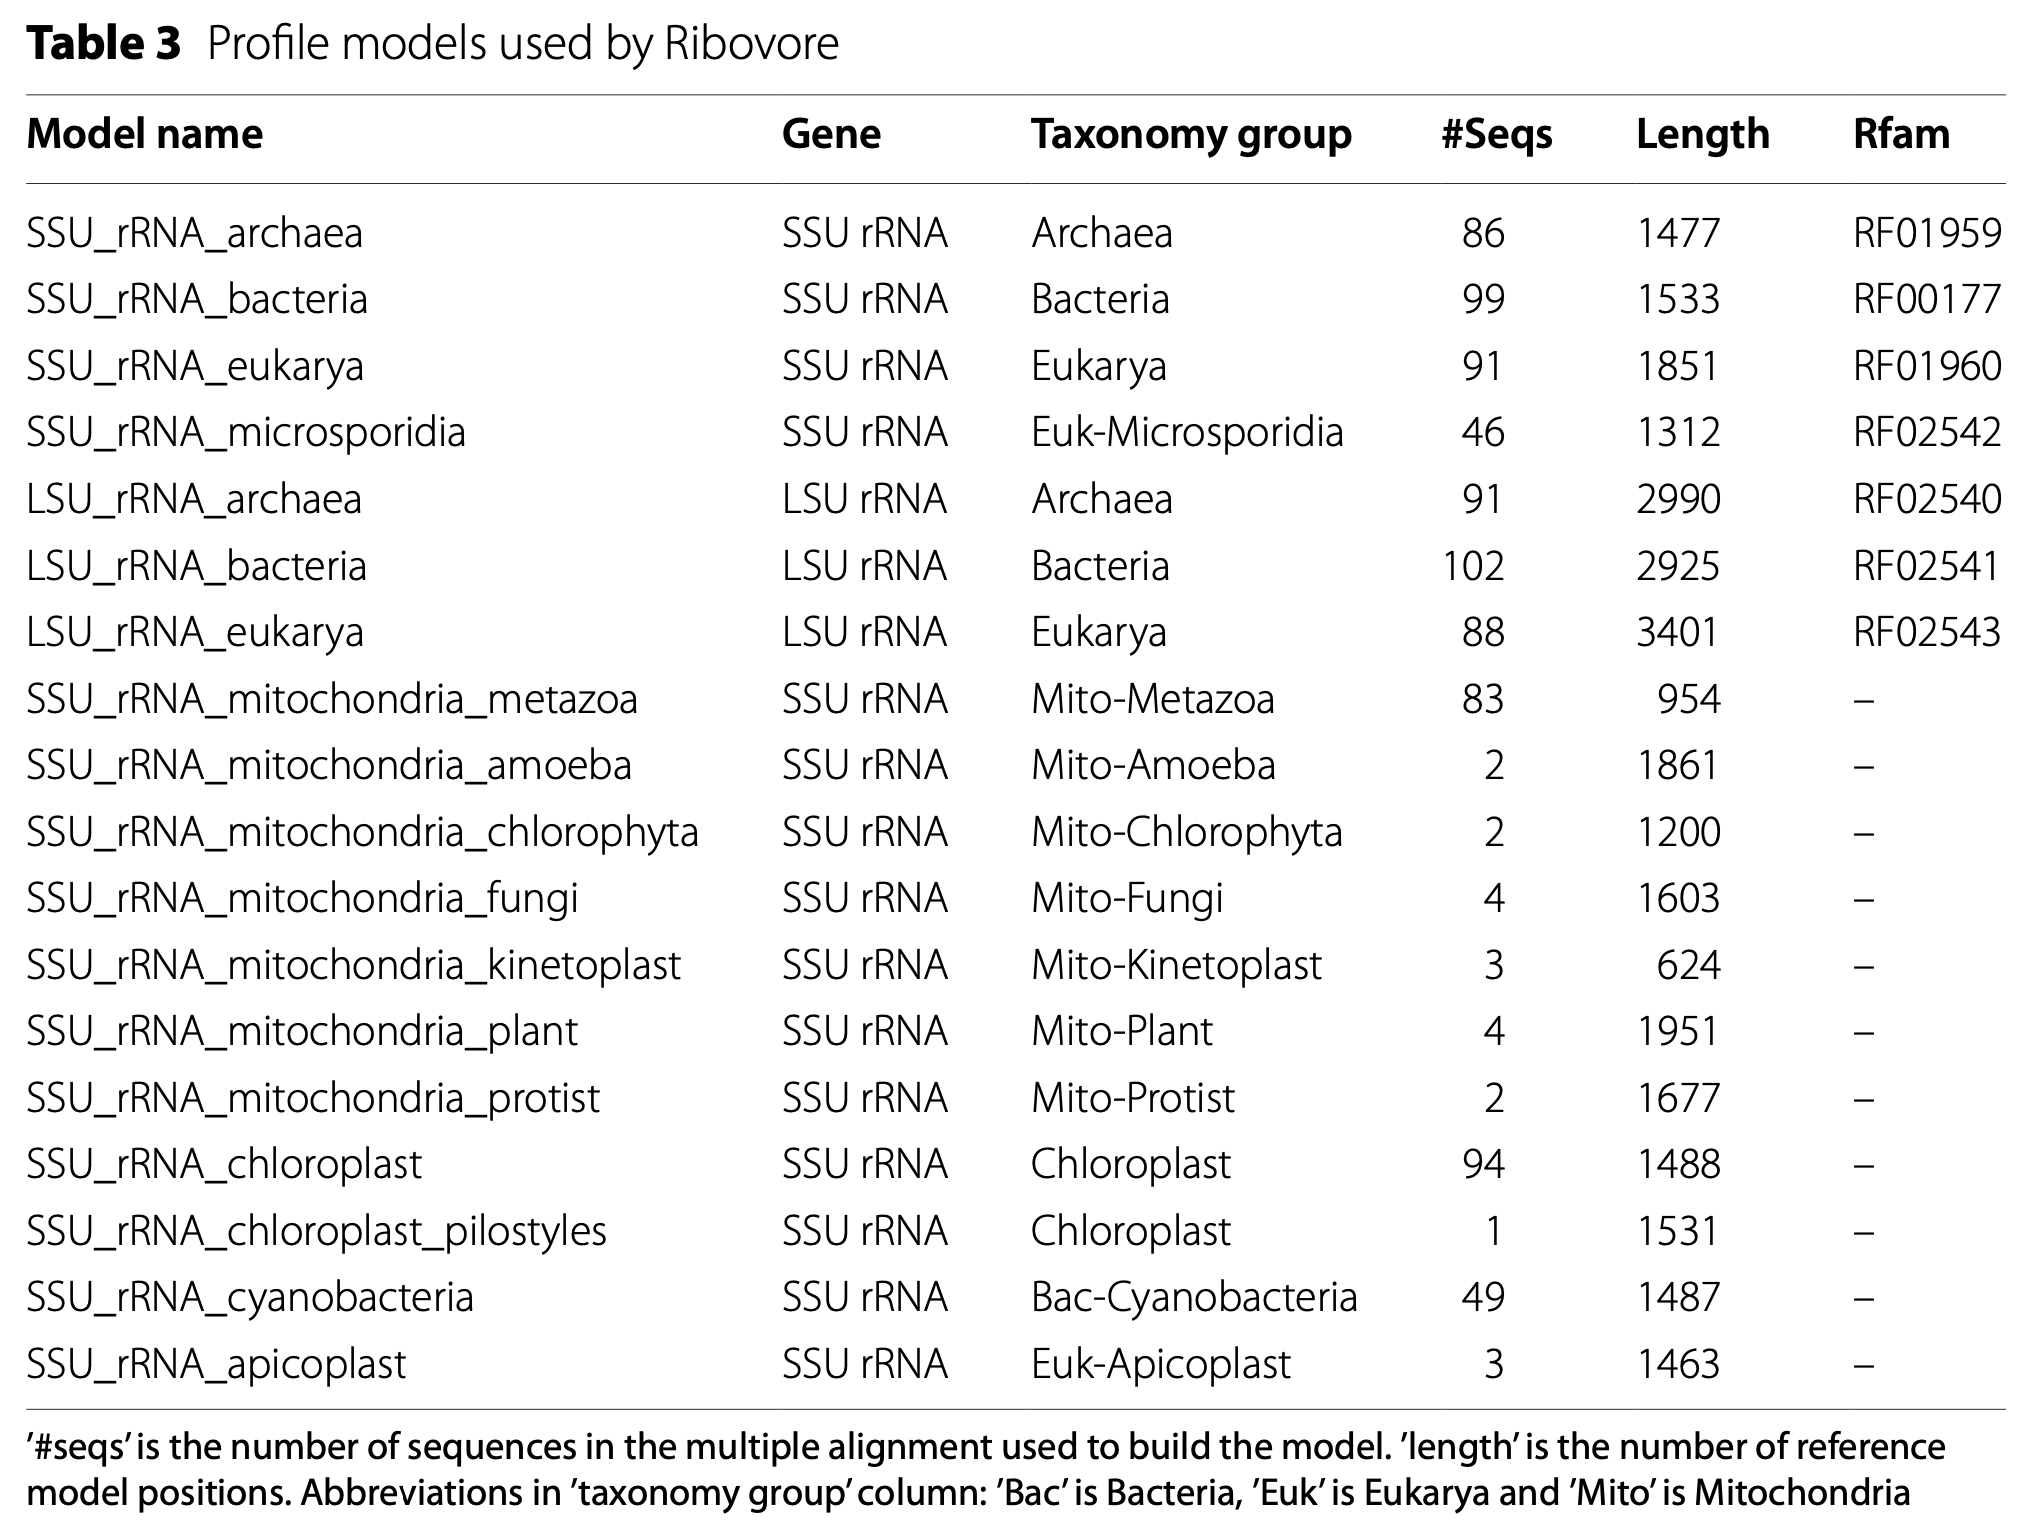
\includegraphics[width=9in]{figs/ribovore-table3}
\end{center}

\vfill
\end{slide}
%%%%%%%%%%%%%%%%%%%%%%%%%%%%%%%%%%%%%%%%%%%%%%%%%%%%%%%%%%%%%%%%%%%%%%


\begin{slide}

\large
\begin{center}
\large{\textbf{Acknowledgements}} \\

\normalsize
\vspace{0.75in}

\small
\begin{tabular}{l|l|l}
%                  & \\ \hline
%                  & \\
\textbf{NCBI - viral annotation} & \textbf{NCBI - leadership} &  \textbf{Software developers} \\
Alejandro Sch\"{a}ffer (now NCI) & David Landsman             & Sean Eddy (HMMER/Infernal/Easel)\\
                                 & Kim Pruitt                 & Travis Wheeler (HMMER)\\
Linda Yankie                     & Steve Sherry               & Tom Madden and BLAST team \\
Vincent Calhoun                  & Jim Ostell                 & William Pearson (FASTA/glsearch) \\
Sergiy Gotvyanskyy               & David Lipman               & Michael Farrar (HMMER/glsearch) \\
Susan Schafer                    &                            & \\
Ilene Mizrachi                   & \textbf{NLM - leadership}  & \\
Colleen Bollin                   & Patti Brennan              & This research was supported by \\
Beverly Underwood                & Jerry Sheehan              & the Intramural Research Program \\
Prakash Keranahalli              & Valerie Florance           & of the NIH, National Library \\
Vasuki Gobu                      &                            & of Medicine. \\
Alex Kotliarov                   & & \\
& & \\
Rodney Brister                   & & \\
Eneida Hatcher                   & & \\
& & \\
Lara Shonkwiler                  & & \\
Sophia Hu                        & & \\
& & \\
Wratko Hlavina                   & & \\
Ron Patterson                    & & \\
\end{tabular}


\includegraphics[width=2.5in]{figs/NIH_NLM_ABRV_2C_4-white}

\includegraphics[width=2.5in]{figs/ncbi-logo}

\end{center}

\vfill
\end{slide}


\end{document}
%%%%%%%%%%%%%%%%%%%%%%%%%%%%%%%%%%%%%%%%%%%%%%%%%%%%%%%%%%%%%%%%%%%%%%
%%%%%%%%%%%%%%%%%%%%%%%%%%%%%%%%%%%%%%%%%%%%%%%%%%%%%%%%%%%%%%%%%%%%%%
%%%%%%%%%%%%%%%%%%%%%%%%%%%%%%%%%%%%%%%%%%%%%%%%%%%%%%%%%%%%%%%%%%%%%%
%%%%%%%%%%%%%%%%%%%%%%%%%%%%%%%%%%%%%%%%%%%%%%%%%%%%%%%%%%%%%%%%%%%%%%
%%%%%%%%%%%%%%%%%%%%%%%%%%%%%%%%%%%%%%%%%%%%%%%%%%%%%%%%%%%%%%%%%%%%%%
%%%%%%%%%%%%%%%%%%%%%%%%%%%%%%%%%%%%%%%%%%%%%%%%%%%%%%%%%%%%%%%%%%%%%%
\begin{slide}
\begin{center}
\textbf{Sequence submissions are handled by expert NCBI indexers}
\end{center}

\small
\begin{itemize}
\item Indexers check submissions for quality
\item Many submissions are of \emph{marker genes}, used to
  characterize environments (microbiome, soil), which are
  automatically analyzed by BLAST or specialized tools.
%\item Submissions with zero errors automatically enter database
%  (``foosh'')
%\item Submissions with errors can be corrected by submitter or are manually reviewed by an indexer
\end{itemize}

\medskip

\begin{center}
\begin{tabular}{l||r|r||r||l}
                                 &    2018  & total     &         &           \\
 marker gene/                    &  GenBank & GenBank   &  TLS\footnote{TLS: Targeted Locus Study, currently only 16S submissions with $>=$ 2500 seqs}      & analysis  \\
 sequence type                   &  \# seqs & \# seqs   & \# seqs & tool \\ \hline
& & & \\                    
%\textcolor{red}{16S rRNA}        & \textcolor{red}{333,121}  & \textcolor{red}{8,015,297} & \textcolor{red}{18,262,402} & \textcolor{red}{BLAST}\footnote{TLS submissions now processed with Ribosensor} \\
%16S rRNA                        & 333,121  & 8,015,297 & 18,262,402 & BLAST$^{*}$ \\
16S rRNA                        & 333,121  & 8,015,297 & 18,262,402 & BLAST \\
& & & \\                    
 23S rRNA                        & 74,287  &   275,014  & 2,140      & BLAST \\
& & & \\
 ITS1                            & 27,279  &   359,380  & 13,294     & BLAST \\
& & & \\                    
 ITS2                            & 24,144  &   184,515  &      0     & BLAST \\
& & & \\                    
 ITS1+ITS2                       & 26,734  &   445,721  & 25,725     & BLAST \\
& & & \\                    
 Influenza A                     & 74,868  &   665,464  &      0     & FLAN \\
\end{tabular}
\end{center}
\vfill
\tiny \flushleft{$\dagger$ TLS: Targeted Locus Study, currently only 16S submissions with $>=$ 2500 seqs, handled by Anji Johnston}
%\tiny \flushleft{$\ddagger$ TLS submissions now processed with ribosensor}
\end{slide}


%%%%%%%%%%%%%%%%%%%%%%%%%%%%%%%%%%%%%%%%%%%%%%%%%%%%%%%%%%%%%%%%%%%%%%
\begin{slide}
\begin{center}

\includegraphics[width=10.5in]{figs/ss-vapid-title}
\end{center}

\small
\begin{itemize}
\item large reference database of nearly all complete genomes in
  GenBank
\item annotates each sequence based on best-match in reference
  database using blastn
\item designed for complete viral genomes
\item identifies early and absent stop codons and frameshift indels
\item simplifies submission by adding metadata expected by GenBank
\end{itemize}

\vfill
\end{slide}
%%%%%%%%%%%%%%%%%%%%%%%%%%%%%%%%%%%%%%%%%%%%%%%%%%%%%%%%%%%%%%%%%%%%%%
\begin{slide}
\begin{center}

\includegraphics[width=10.5in]{figs/ss-vigor-title}
\end{center}

\small
\begin{itemize}
\item determines most appropriate database (e.g. Norovirus)
  and annotates based on comparison of all proteins and mature
  peptides in that database
\item no Dengue database
\item identifies early and absent stop codons and frameshift indels
\end{itemize}

\vfill
\end{slide}
%%%%%%%%%%%%%%%%%%%%%%%%%%%%%%%%%%%%%%%%%%%%%%%%%%%%%%%%%%%%%%%%%%%%%%
\begin{slide}
\begin{center}
\textbf{Summary of VAPiD, VIGOR and VADR on 200 randomly chosen seqs}

\begin{tabular}{|l|r|r|r|}
\hline
         & VADR       & VAPiD     & VIGOR      \\
 dataset & pass/fail  & pass/fail & pass/fail  \\ \hline
       NC &  167/33 &  161/39 &   198/2 \\ 
       DC &  189/11 &   196/4 &       - \\ 
       NP &   191/9 &       - &   195/5 \\ 
       DP &  163/37 &       - &       - \\ 
\hline 
\end{tabular}
\end{center}

\vfill
\end{slide}
%%%%%%%%%%%%%%%%%%%%%%%%%%%%%%%%%%%%%%%%%%%%%%%%%%%%%%%%%%%%%%%%%%%%%%
\begin{slide}
\begin{center}
\textbf{Comparison of VAPiD and VADR}

\begin{tabular}{|l|r|r|r|r|}
\hline
          & Both       & Both       & VADR-pass  & VADR-fail  \\
 dataset  & pass       & fail       & VAPiD-fail & VAPiD-pass \\ \hline
       NC &        137 &          9 &         30 &     24 \\ 
       DC &        188 &          3 &          1 &      8 \\ 
\hline 
\end{tabular}

\end{center}

\vfill
\end{slide}
%%%%%%%%%%%%%%%%%%%%%%%%%%%%%%%%%%%%%%%%%%%%%%%%%%%%%%%%%%%%%%%%%%%%%%
\begin{slide}
\begin{center}
\textbf{Comparison of VAPiD and VADR}

\begin{tabular}{|l|r|r|r|r|}
\hline
          & Both       & Both       & VADR-pass  & VADR-fail  \\
 dataset  & pass       & fail       & VAPiD-fail & VAPiD-pass \\ \hline
       NC &        137 &          9 &         30 &     24 \\ 
       DC &        188 &          3 &          1 &      8 \\ 
\hline 
\end{tabular}

\small
\begin{itemize}
\item 12 that fail both:
  \begin{itemize}
  \item 9 have an internal stop or another
    CDS translation problem
  \item one has a start codon problem
  \item one is reverse complemented
  \item one fails because no reference is found
  \end{itemize}
\item 31 that fail only VAPiD are:
  \begin{itemize}
  \item 5' and/or 3' truncated in the first or final CDS
  \item 
    otherwise valid according to the VADR and VIGOR results
  \end{itemize}
\item \textcolor{red}{Conclusion: VADR finds all problems that VAPiD finds that should
  be caught.}
\end{itemize}
\end{center}

\vfill
\end{slide}
%%%%%%%%%%%%%%%%%%%%%%%%%%%%%%%%%%%%%%%%%%%%%%%%%%%%%%%%%%%%%%%%%%%%%%
\begin{slide}
\begin{center}
\textbf{Comparison of VIGOR and VADR}

\begin{tabular}{|l|r|r|r|r|}
\hline
         & Both       & Both       & VADR-pass  & VADR-fail  \\
 dataset & pass       & fail       & VIGOR-fail & VIGOR-pass \\ \hline
       NC &    167 &      2 &      0 &     31 \\ 
       NP &    191 &      5 &      0 &      4 \\ 
\hline 
\end{tabular}

\end{center}

\vfill
\end{slide}
%%%%%%%%%%%%%%%%%%%%%%%%%%%%%%%%%%%%%%%%%%%%%%%%%%%%%%%%%%%%%%%%%%%%%%
\begin{slide}
\begin{center}
\textbf{Comparison of VIGOR and VADR}

\begin{tabular}{|l|r|r|r|r|}
\hline
         & Both       & Both       & VADR-pass  & VADR-fail  \\
 dataset & pass       & fail       & VIGOR-fail & VIGOR-pass \\ \hline
      NC &        167 &          2 &          0 &     31 \\ 
      NP &        191 &          5 &          0 &      4 \\ 
\hline 
\end{tabular}

\small
\begin{itemize}
\item 7 that fail both:
  \begin{itemize}
  \item 3 have premature stops
  \item 2 are reverse complemented
  \item one has a frameshift 
  \item one fails because no similar reference is found
  \end{itemize}
\item \textcolor{red}{Conclusion: VADR finds all problems that VIGOR finds that should
  be caught.}
\end{itemize}
\end{center}

\vfill
\end{slide}

%%%%%%%%%%%%%%%%%%%%%%%%%%%%%%%%%%%%%%%%%%%%%%%%%%%%%%%%%%%%%%%%%%%%%%
\begin{slide}
\begin{center}
\textbf{35 sequences in NC, DC, and NP fail only VADR}

\small
\begin{itemize}
\item \textcolor{red}{These all have issues indexers want to manually review:}
\begin{itemize}
\item 16 sequences with early stops compared to closest RefSeqs %(\emph{cdsstopn})
\item 12 sequences for which BLASTX alignment does not extend close
  enough to alignment-based prediction %(\emph{indf5pst}, \emph{indf3pst})
\item 10 sequences with low similarity to RefSeq at 5' or 3' end of
  sequence or a feature %(lowsim5f, lowsim3f, or lowsim3s alerts)
\item 7 sequences where 5' or 3' boundary is a gap or not aligned with
  sufficient confidence (high enough posterior probability)
  %(indf5loc, indf5gap, or indf3loc alerts)
\item 5 sequences that are expected to be Norovirus but are really Sapovirus
  %(incgroup alerts)
\item 5 sequences with too large of an insertion/deletion in the
  BLASTX alignment %(insertnp or deletinp alerts)
\item 1 sequence not recognized by any of the \emph{Caliciviridae} or
  \emph{Flaviviridae} models (a Salivirus from \emph{Picornaviridae}
  family) %(noannotn alert)
\end{itemize}
\end{itemize}
\end{center}

\vfill
\end{slide}
\begin{slide}
\begin{center}
\textbf{VADR build step (\texttt{v-build.pl}) builds a homology model
  \\ (covariance model (CM)) of a RefSeq and stores feature information}

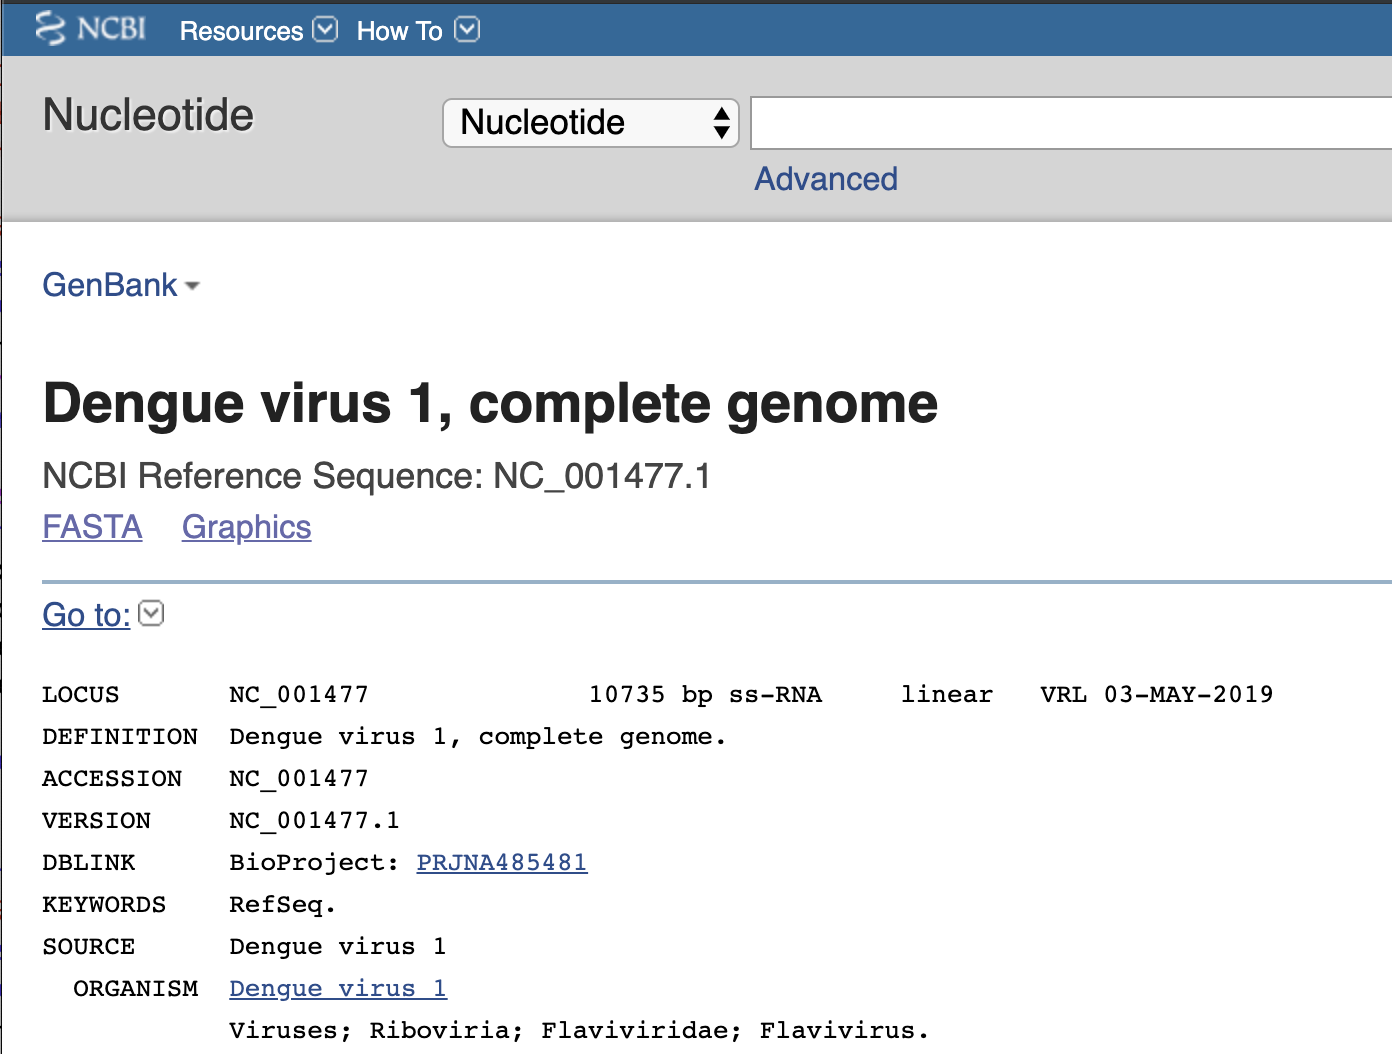
\includegraphics[width=6in]{figs/ss-001477-top}

\end{center}
\vfill
\end{slide}
%%%%%%%%%%%%%%%%%%%%%%%%%%%%%%%%%%%%%%%%%%%%%%%%%%%%%%%%%%%%%%%%%%%%%%
\begin{slide}
\begin{center}
\textbf{VADR build step (\texttt{v-build.pl}) builds a homology model
  \\ (covariance model (CM)) of a RefSeq and stores feature information}

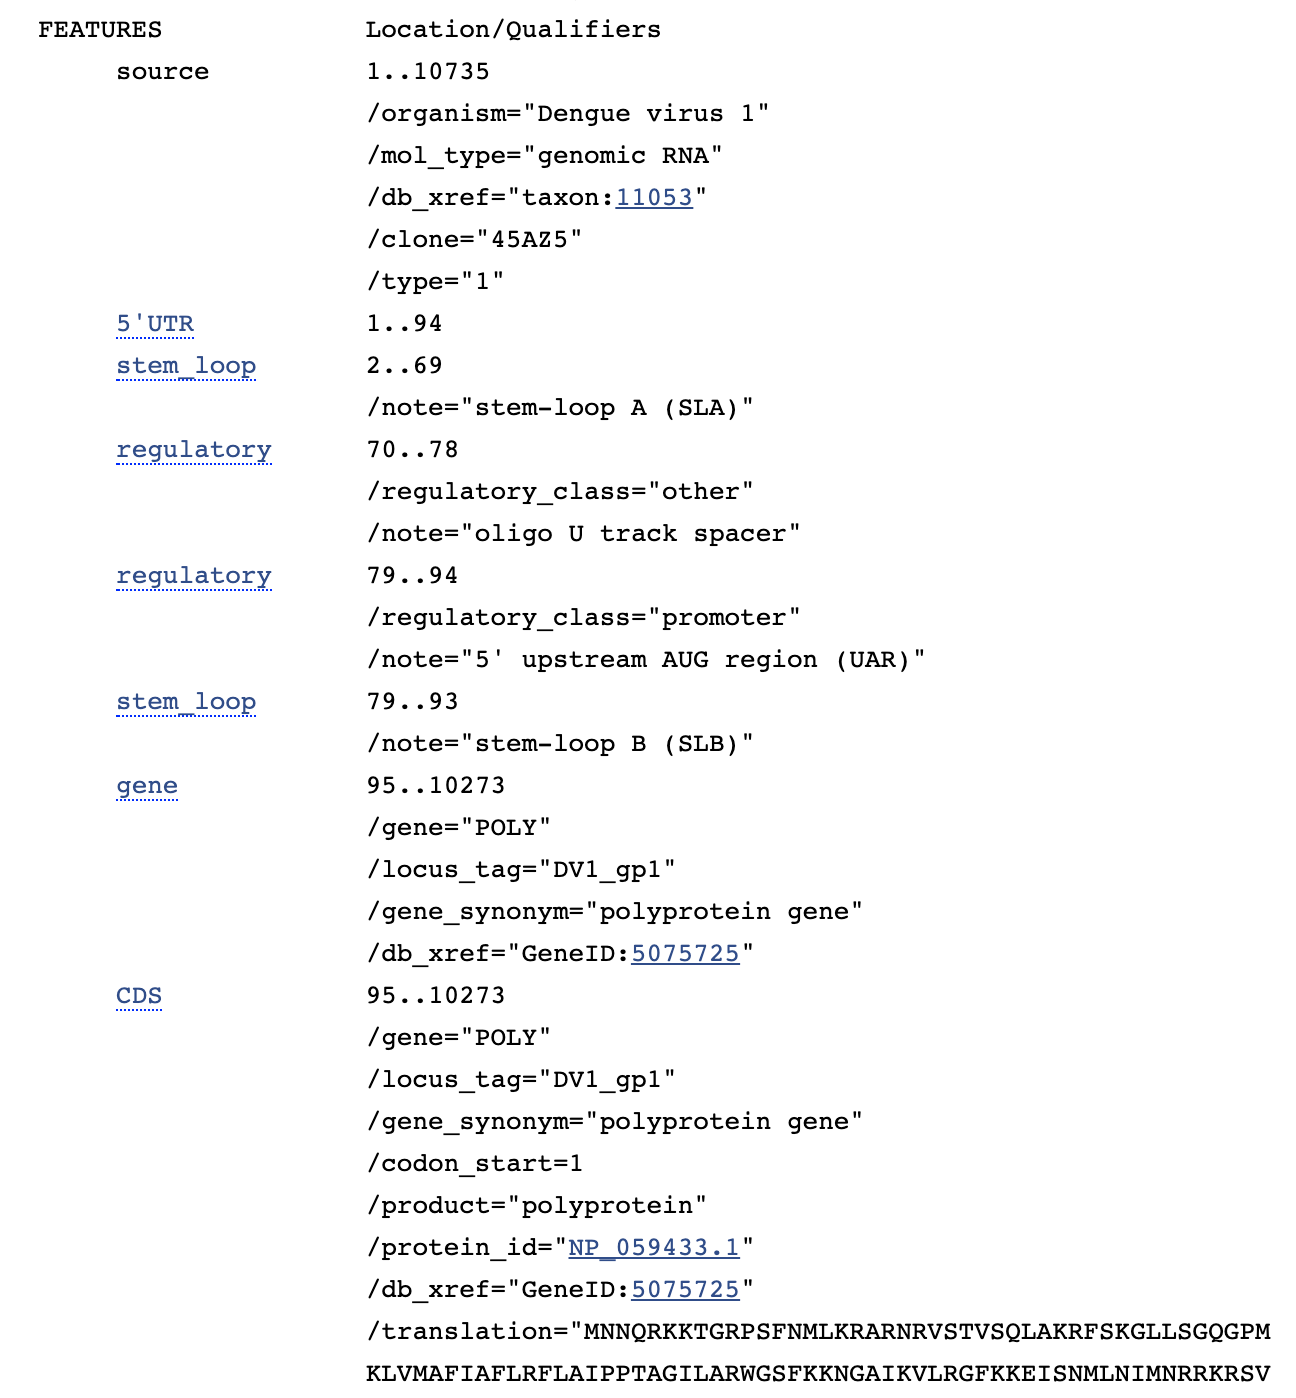
\includegraphics[width=6in]{figs/ss-001477-mid}

\end{center}
\vfill
\end{slide}
%%%%%%%%%%%%%%%%%%%%%%%%%%%%%%%%%%%%%%%%%%%%%%%%%%%%%%%%%%%%%%%%%%%%%%
\begin{slide}
\begin{center}
\textbf{VADR build step (\texttt{v-build.pl}) builds a homology model
  \\ (covariance model (CM)) of a RefSeq and stores feature information}

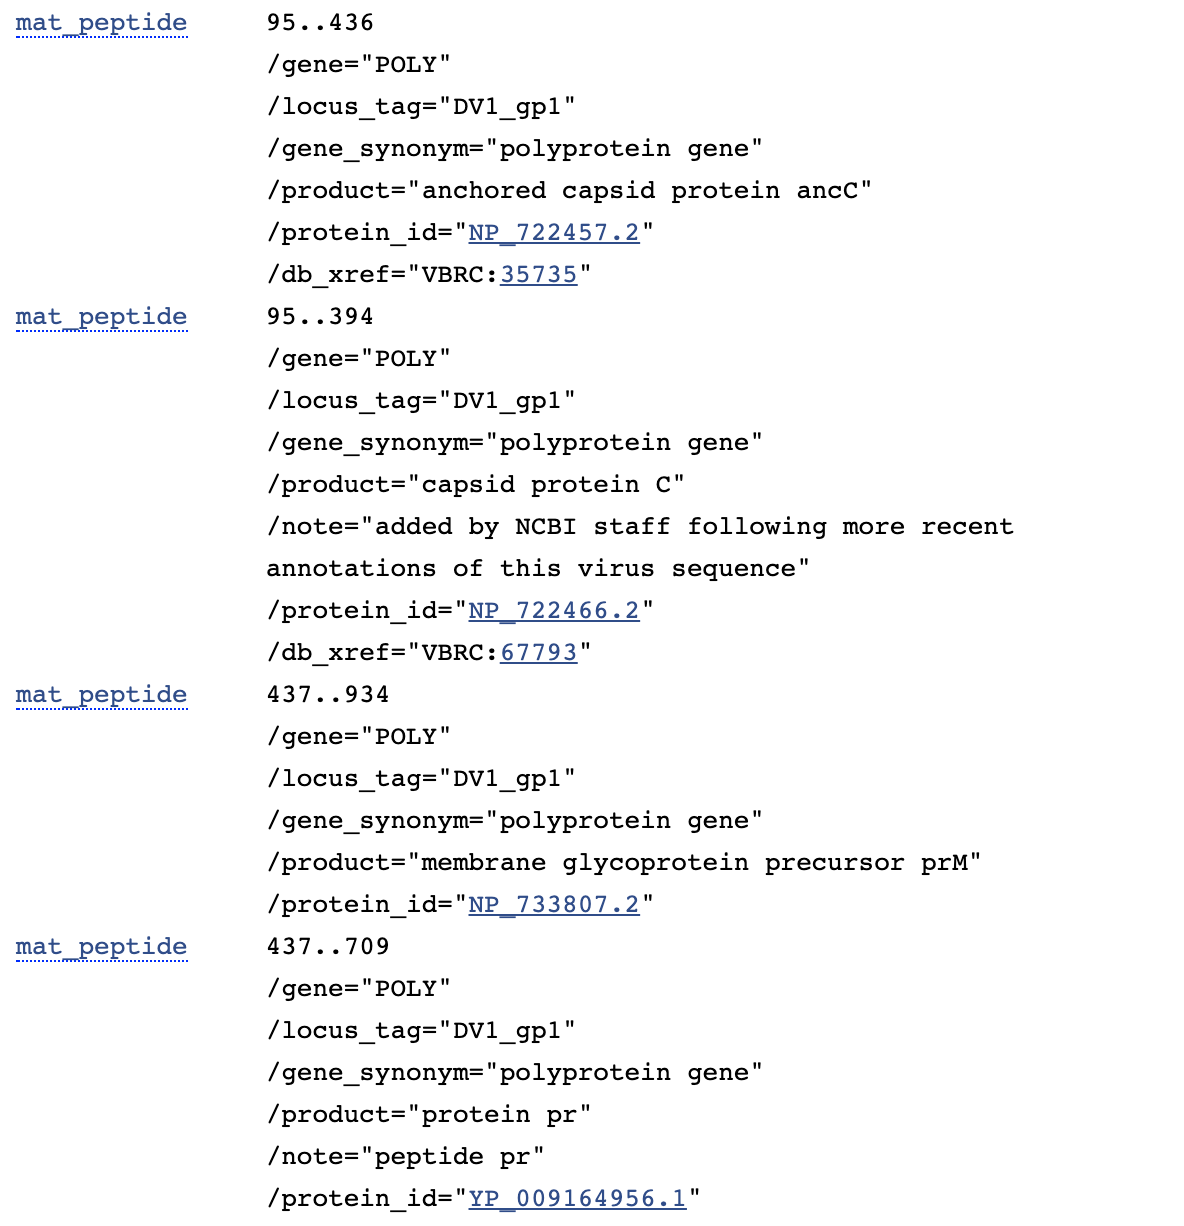
\includegraphics[width=6in]{figs/ss-001477-bot}

\end{center}
\vfill
\end{slide}
%%%%%%%%%%%%%%%%%%%%%%%%%%%%%%%%%%%%%%%%%%%%%%%%%%%%%%%%%%%%%%%%%%%%%%
\begin{slide}
\begin{center}
\textbf{VADR build step (\texttt{v-build.pl}) builds a homology model
  \\ (covariance model (CM)) of a RefSeq and stores feature information}

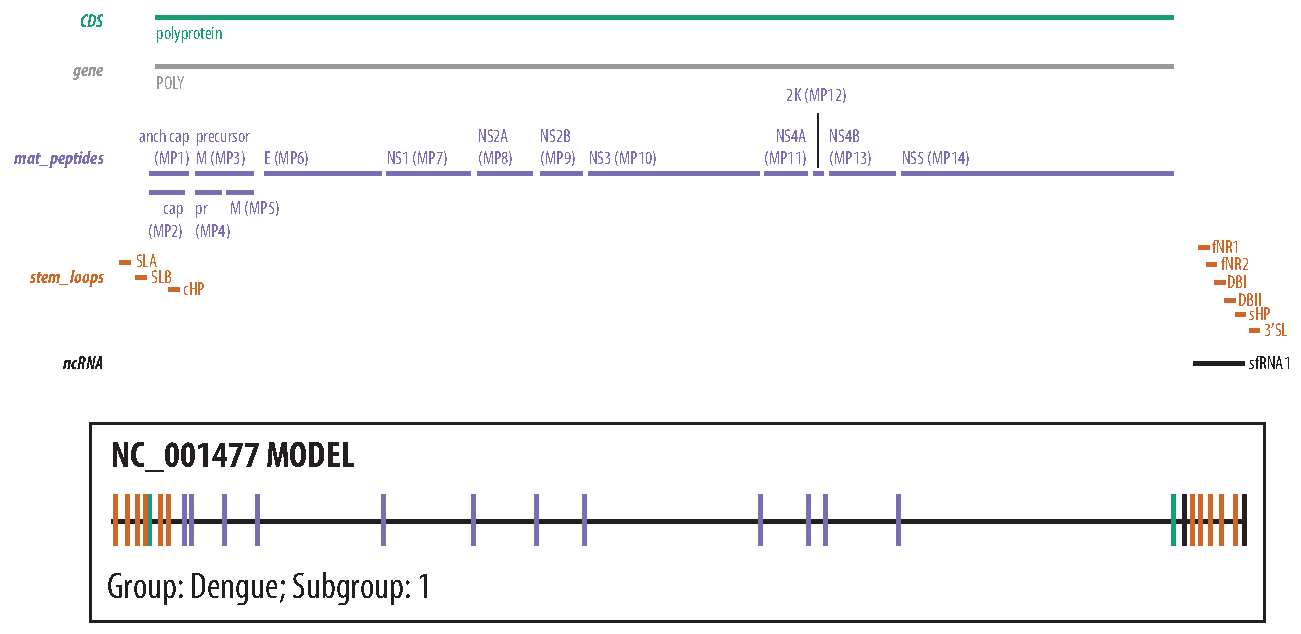
\includegraphics[width=10.5in]{figs/dengue-features}

\end{center}
\vfill
\end{slide}
%%%%%%%%%%%%%%%%%%%%%%%%%%%%%%%%%%%%%%%%%%%%%%%%%%%%%%%%%%%%%%%%%%%%%%
\begin{slide}
\begin{center}
\textbf{VADR build step (\texttt{v-build.pl}) builds a homology model
  \\ (covariance model (CM)) of a RefSeq and stores feature information}

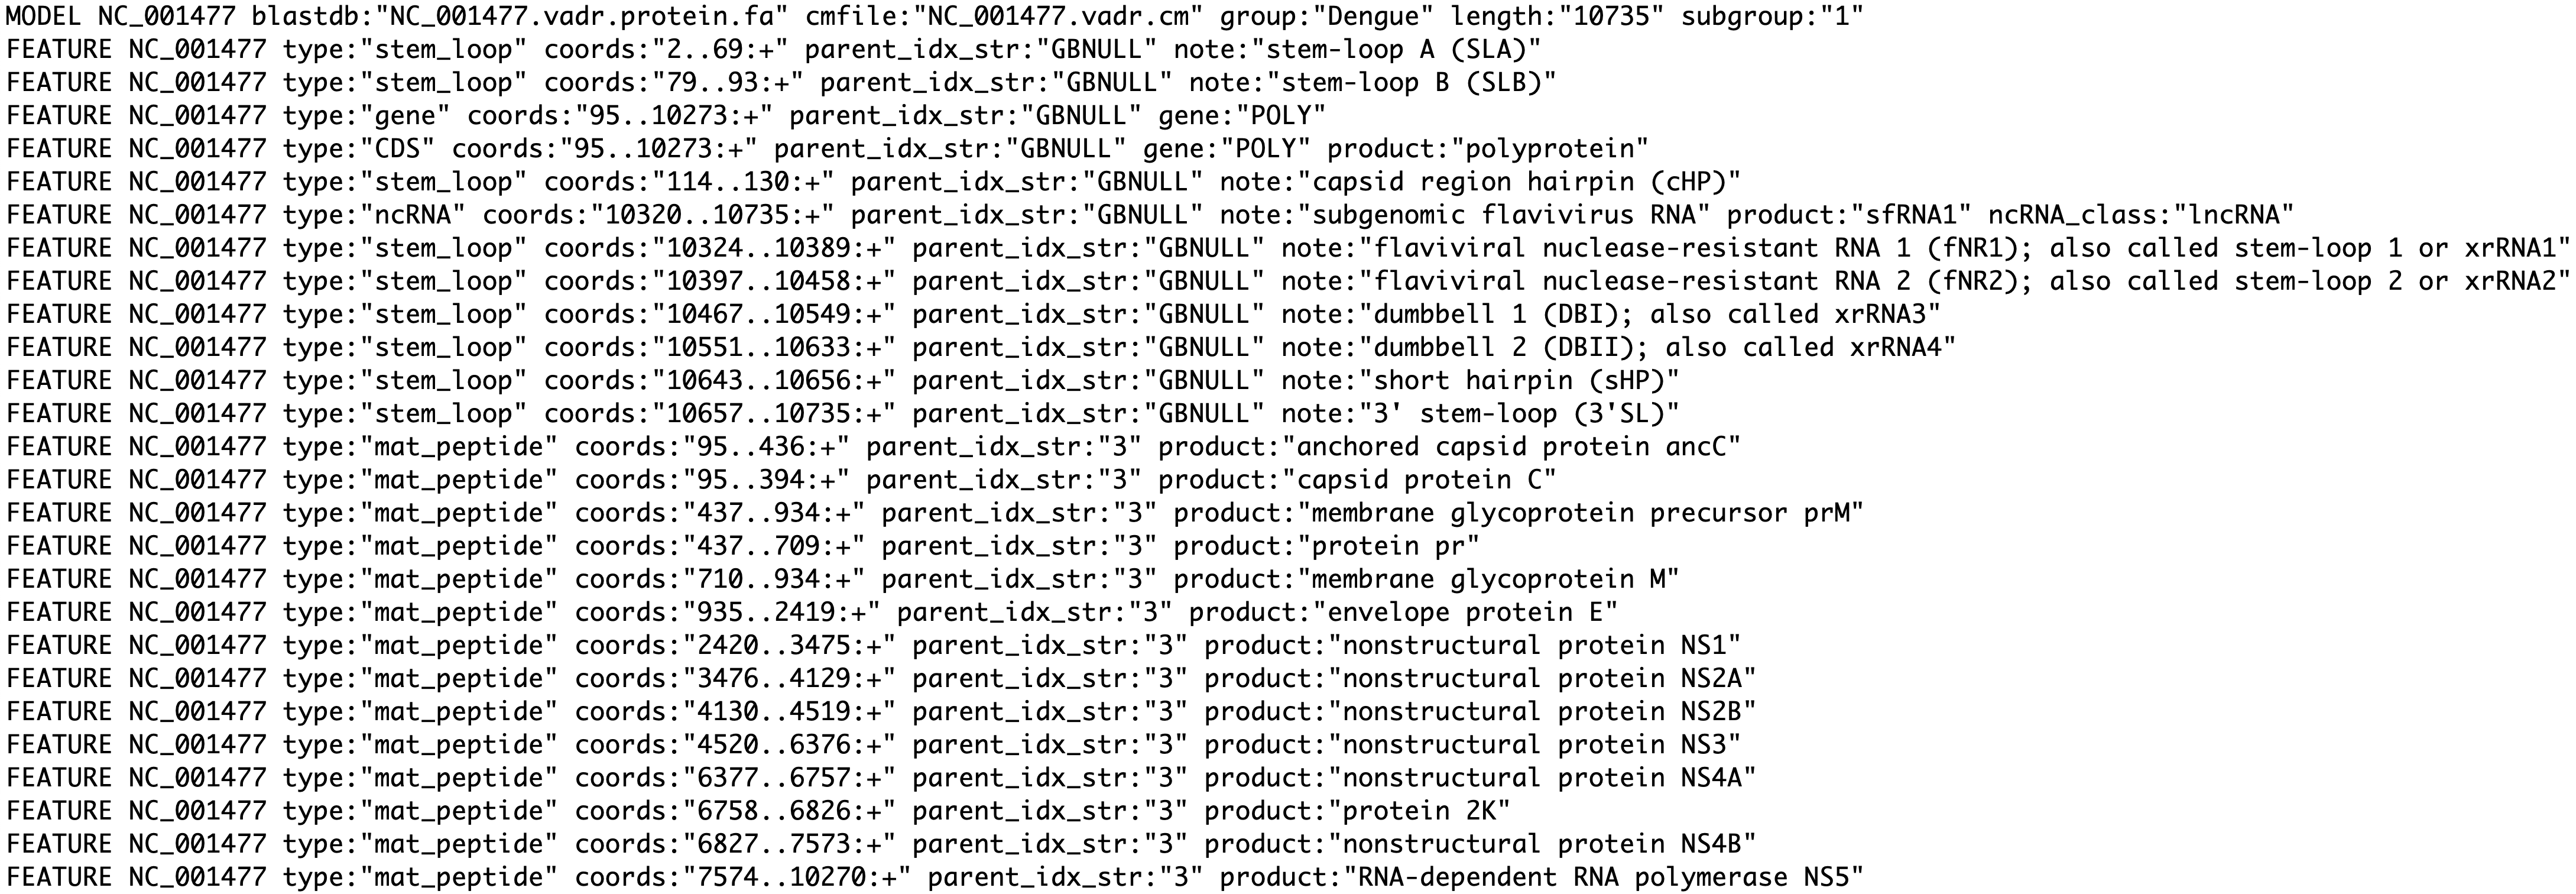
\includegraphics[width=10.5in]{figs/ss-001477-minfo}

\end{center}
\vfill
\end{slide}
%%%%%%%%%%%%%%%%%%%%%%%%%%%%%%%%%%%%%%%%%%%%%%%%%%%%%%%%%%%%%%%%%%%%%%
\begin{slide}
\begin{center}

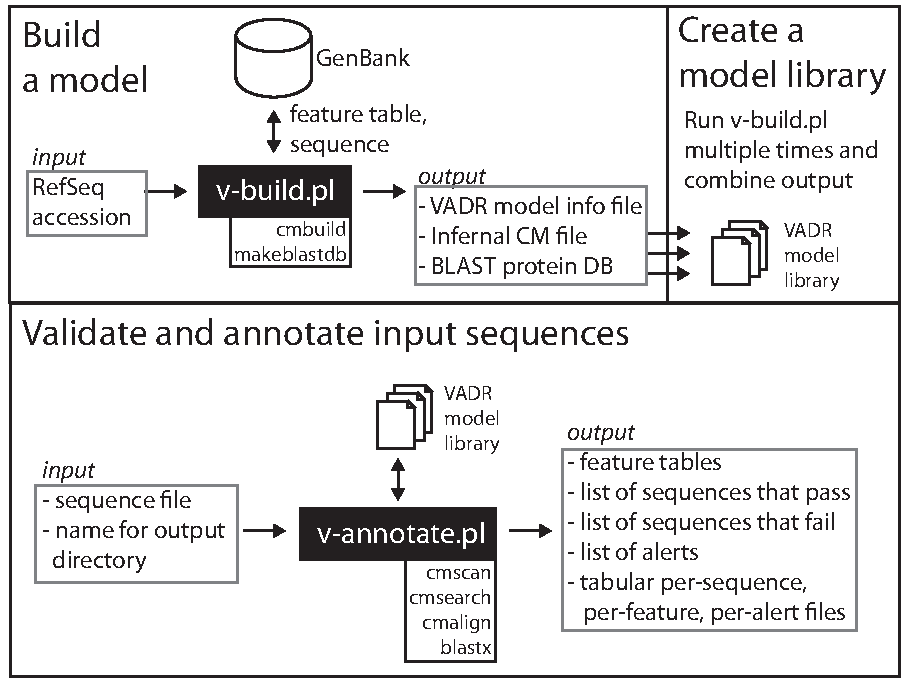
\includegraphics[width=10in]{figs/vadr}

\end{center}
\vfill
\end{slide}
%%%%%%%%%%%%%%%%%%%%%%%%%%%%%%%%%%%%%%%%%%%%%%%%%%%%%%%%%%%%%%%%%%%%%%
\begin{slide}
\begin{center}
\normalsize
\textbf{VADR 1.0 model library}

% /panfs/pan1/infernal/notebook/19_0520_vadr_build_from_ft/00LOG.txt
% 41 of the '197' models are Caliciviridae
% 156 of the '197' models are Flaviviridae
% But we purposefully omitted 3 new Norovirus from Flaviviridae, so
% it's 41 and 153.

\small
\begin{itemize}
\item 38 \emph{Caliciviridae} models:
  \begin{itemize}
  \item \textcolor{red}{9 Norovirus models}
  \item 7 Sapovirus models
  \item 4 Vesivirus models
    %  \item 18 other Caliciviruses
  \end{itemize}
\item 156 \emph{Flaviviridae} models:
  \begin{itemize}
  \item 10 Pegivirus models
%  \item \textcolor{red}{8 HCV models}
  \item 8 HCV models
  \item 7 Pestivirus models
  \item \textcolor{red}{4 Dengue virus models}
  \item 2 West Nile virus models
  \item 2 Zika virus models
  \end{itemize}
\end{itemize}

\end{center}

\vfill
\end{slide}
%%%%%%%%%%%%%%%%%%%%%%%%%%%%%%%%%%%%%%%%%%%%%%%%%%%%%%%%%%%%%%%%%%%%%%
\begin{slide}
\begin{center}
\textbf{\texttt{v-annotate.pl} annotates each sequence using its
  best-matching model}

\begin{itemize}
\item For each sequence $S$:
\small
\begin{enumerate}
\item \textbf{Classification}: compare $S$ to all models to find best matching model $M$
\item \textbf{Coverage determination}: search $M$ against $S$ to find 'hits'
\item \textbf{Alignment}: align $S$ to $M$ and map features from $M$ to $S$
\item \textbf{Protein validation}: compare predicted CDS in $S$ to proteins
  from $M$ using BLASTX
\end{enumerate}
\end{itemize}

\emph{Different types of alerts are identified and reported at each stage}

\end{center}

\vfill
\end{slide}
%%%%%%%%%%%%%%%%%%%%%%%%%%%%%%%%%%%%%%%%%%%%%%%%%%%%%%%%%%%%%%%%%%%%%%
\begin{slide}
\begin{center}

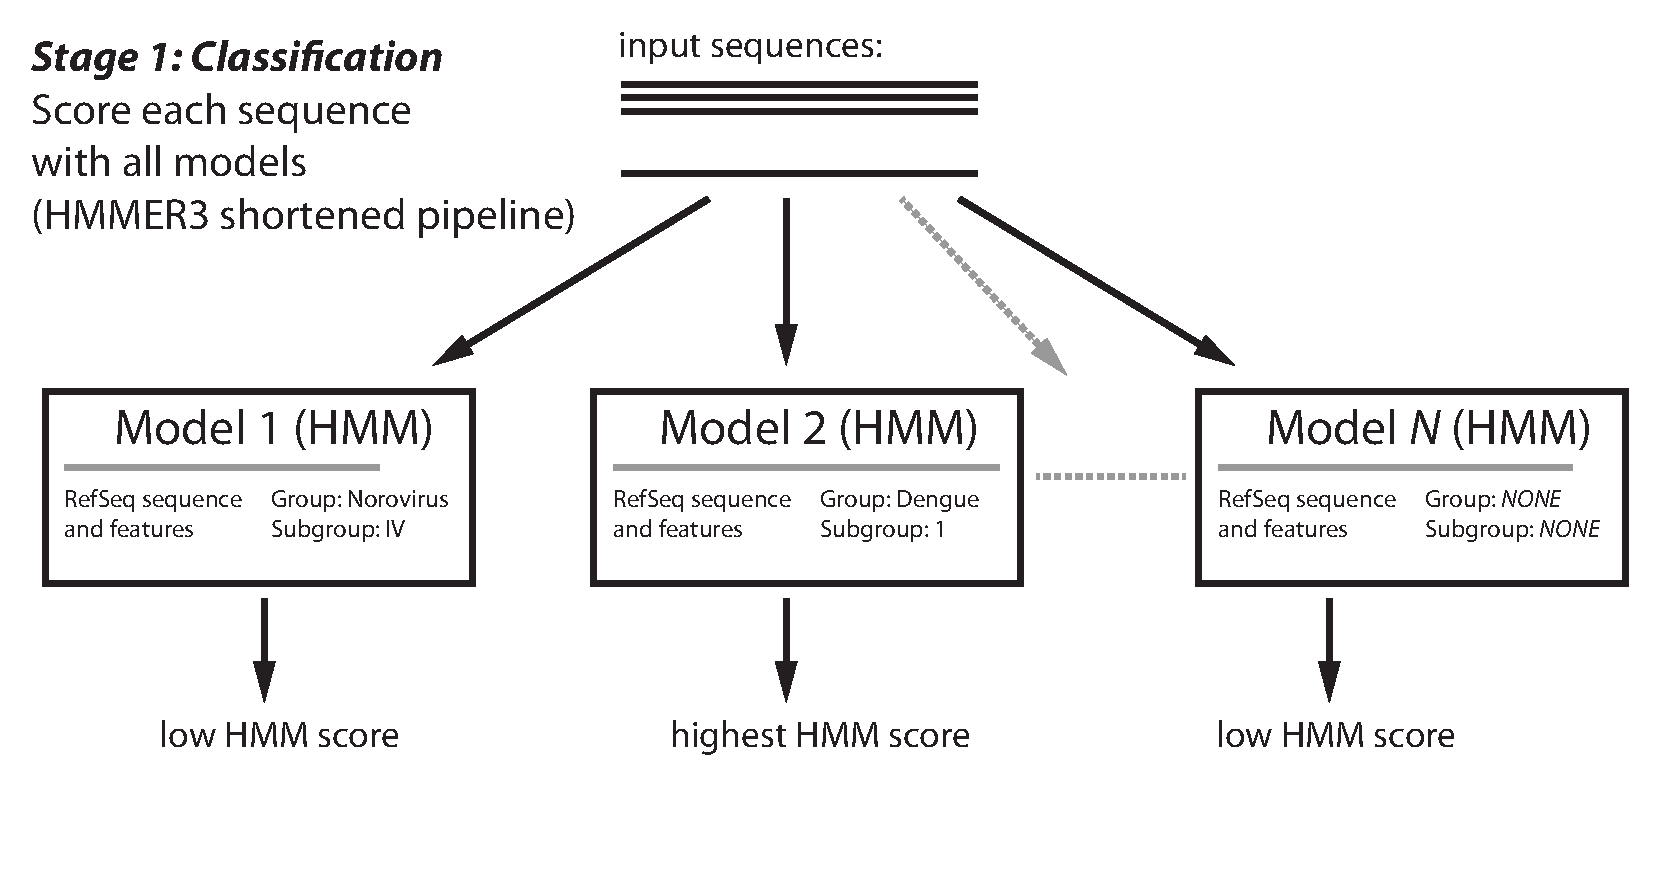
\includegraphics[width=9.5in]{figs/v-annotate-stage1-1}

\end{center}
\vfill
\end{slide}
%%%%%%%%%%%%%%%%%%%%%%%%%%%%%%%%%%%%%%%%%%%%%%%%%%%%%%%%%%%%%%%%%%%%%%
\begin{slide}
\begin{center}

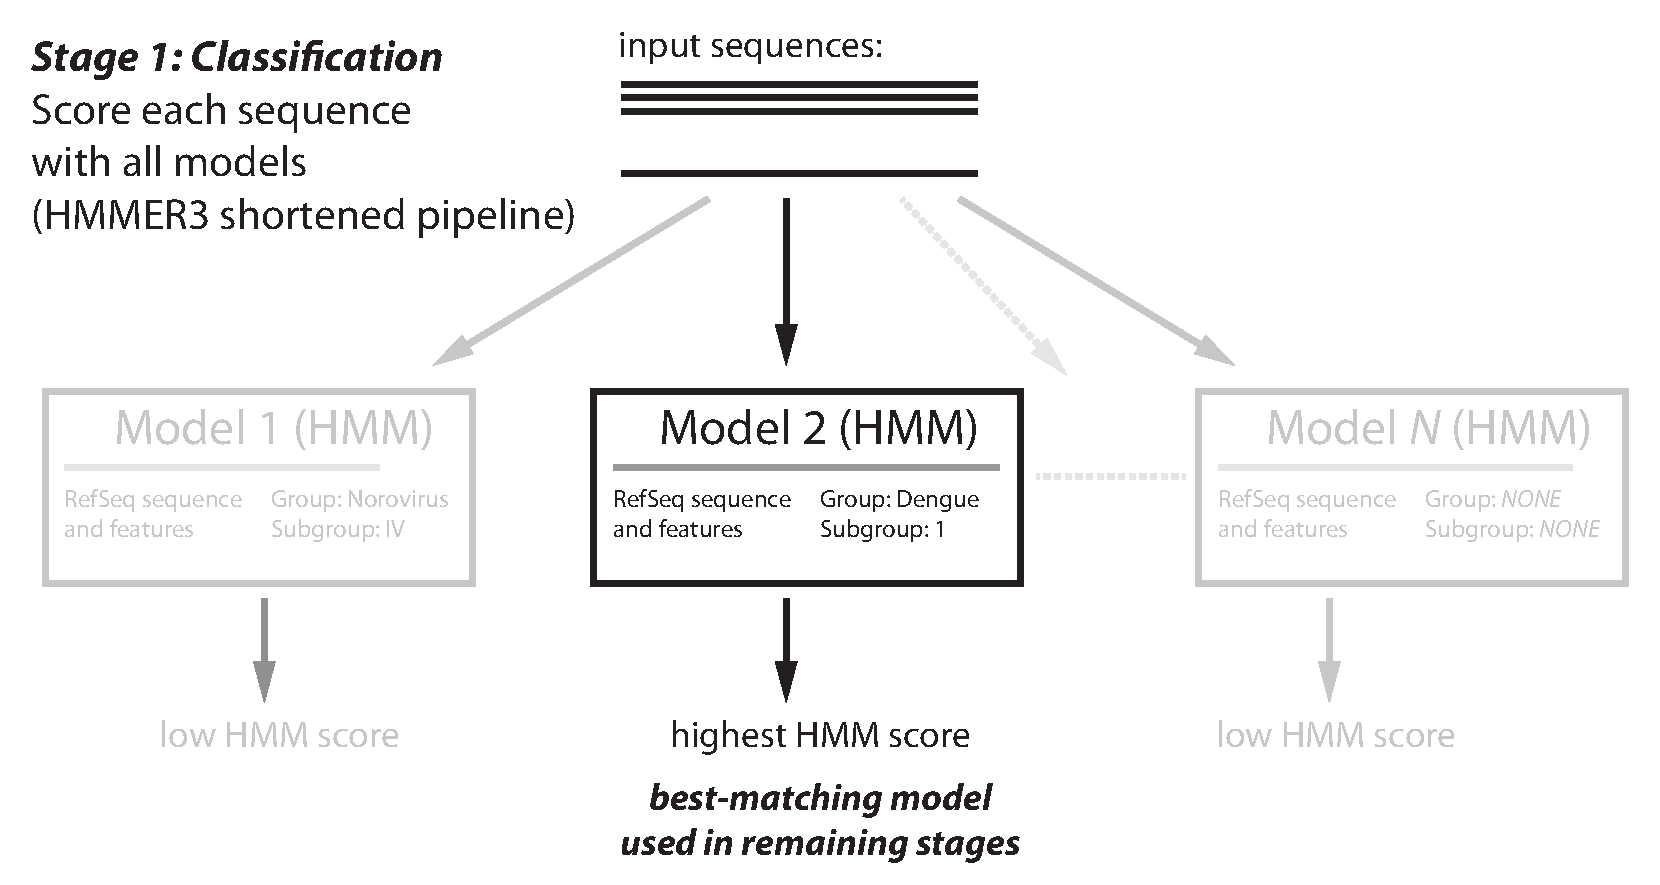
\includegraphics[width=9.5in]{figs/v-annotate-stage1-2}

\end{center}
\vfill
\end{slide}
%%%%%%%%%%%%%%%%%%%%%%%%%%%%%%%%%%%%%%%%%%%%%%%%%%%%%%%%%%%%%%%%%%%%%%
\begin{slide}
\begin{center}

\includegraphics[width=9.5in]{figs/v-annotate-stage1-2}

\includegraphics[width=10.5in]{figs/ss-class-alert-list}

\end{center}
\vfill
\end{slide}
%%%%%%%%%%%%%%%%%%%%%%%%%%%%%%%%%%%%%%%%%%%%%%%%%%%%%%%%%%%%%%%%%%%%%%
\begin{slide}
\begin{center}

\includegraphics[width=10.5in]{figs/v-annotate-stage2-1}

\end{center}
\vfill
\end{slide}
%%%%%%%%%%%%%%%%%%%%%%%%%%%%%%%%%%%%%%%%%%%%%%%%%%%%%%%%%%%%%%%%%%%%%%
\begin{slide}
\begin{center}

\includegraphics[width=10.5in]{figs/v-annotate-stage2-2}
\includegraphics[width=10in]{figs/ss-coverage-alert-list}
\end{center}

\vfill
\end{slide}
%%%%%%%%%%%%%%%%%%%%%%%%%%%%%%%%%%%%%%%%%%%%%%%%%%%%%%%%%%%%%%%%%%%%%%
\begin{slide}
\begin{center}

\includegraphics[width=10.5in]{figs/v-annotate-stage3-1}
\end{center}

\vfill
\end{slide}
%%%%%%%%%%%%%%%%%%%%%%%%%%%%%%%%%%%%%%%%%%%%%%%%%%%%%%%%%%%%%%%%%%%%%%
\begin{slide}
\begin{center}

\includegraphics[width=10.5in]{figs/v-annotate-stage3-2}
\end{center}

\vfill
\end{slide}
%%%%%%%%%%%%%%%%%%%%%%%%%%%%%%%%%%%%%%%%%%%%%%%%%%%%%%%%%%%%%%%%%%%%%%
\begin{slide}
\begin{center}

\includegraphics[width=10.5in]{figs/v-annotate-stage3-3}
\end{center}

\vfill
\end{slide}
%%%%%%%%%%%%%%%%%%%%%%%%%%%%%%%%%%%%%%%%%%%%%%%%%%%%%%%%%%%%%%%%%%%%%%
\begin{slide}
\begin{center}

\includegraphics[width=10.5in]{figs/v-annotate-stage3-4}
\includegraphics[width=10.5in]{figs/ss-alignment-alert-list}

\end{center}
\vfill
\end{slide}
%%%%%%%%%%%%%%%%%%%%%%%%%%%%%%%%%%%%%%%%%%%%%%%%%%%%%%%%%%%%%%%%%%%%%%
\begin{slide}
\begin{center}

\includegraphics[width=10.5in]{figs/v-annotate-stage4-1}

\end{center}
\vfill
\end{slide}
%%%%%%%%%%%%%%%%%%%%%%%%%%%%%%%%%%%%%%%%%%%%%%%%%%%%%%%%%%%%%%%%%%%%%%
\begin{slide}
\begin{center}

\includegraphics[width=10.5in]{figs/v-annotate-stage4-2}
\includegraphics[width=10.5in]{figs/ss-protein-alert-list}

\end{center}
\vfill
\end{slide}
%%%%%%%%%%%%%%%%%%%%%%%%%%%%%%%%%%%%%%%%%%%%%%%%%%%%%%%%%%%%%%%%%%%%%%
\begin{slide}

\includegraphics[width=7in]{figs/blank-slide}
  
\vfill
\end{slide}
